%This template was prepared by Dorothea F. Brosius of the 
%Institute for Electronics and Applied Physics, University of Maryland, College Park, MD
%The template was last updated in March 2013
%Thesis Main Page used with thesis.sty based on the
%University of Maryland Electronic Thesis and Dissertation (ETD) Style Guide

\documentclass[12pt]{thesis}  %12pt is larger than 11pt
%\usepackage[pctex32]{graphics}
\usepackage{titlesec}
   \titleformat{\chapter}
      {\normalfont\large}{Chapter \thechapter:}{1em}{}

\usepackage{longtable}
\usepackage{graphicx}
\usepackage{cite}
\usepackage{notoccite}
\usepackage{lscape}
\usepackage{indentfirst}
%\usepackage{latexsym}
\usepackage{multirow}
%\usepackage{tabls}
\usepackage{wrapfig}
\usepackage{slashbox}
\usepackage{supertabular}
%\usepackage{subeqn}
\usepackage{subfigure}
\usepackage{amsmath}
\usepackage{amssymb}
\usepackage{xspace}
\usepackage{setspace}
\usepackage[pagebackref=true,breaklinks=true,linktocpage=true,pdfstartview=FitH,plainpages=false,pdfpagelabels]{hyperref}

%%%%%%%%%%%%% ptdr definitions %%%%%%%%%%%%%%%%%%%%%
\usepackage{ptdr-definitions}
%%%%%%%%%%%%% Symbols %%%%%%%%%%%%%%%%%%%
%math
%\newcommand\triplet[3]{\left(\genfrac{}{}{0pt}{0}{#1}{\genfrac{}{}{0pt}{0}{#2}{#3}}\right)}
\newcommand\triplet[4][c]{\left(%
        \begin{array}{@{}#1@{}}#2\\#3\\#4%
\end{array}%
\right)%
}
\newcommand\doublet[3][c]{\left(%
        \begin{array}{@{}#1@{}}#2\\#3%
\end{array}%
\right)%
}

\newcommand{\neghphantom}[1]{\settowidth{\dimen0}{#1}\hspace*{-\dimen0}}

\newcommand{\tauh}{\ensuremath{\tau_{\text{h}}}\xspace}
\newcommand{\Pe}{\ensuremath{\cmsSymbolFace{e}}\xspace}
\newcommand{\Pep}{\ensuremath{\cmsSymbolFace{e}^{+}}\xspace}
\newcommand{\Pem}{\ensuremath{\cmsSymbolFace{e}^{-}}\xspace}
\newcommand{\Pp}{\ensuremath{\cmsSymbolFace{p}}\xspace}
\newcommand{\mutau}{\ensuremath{\mu\tauh}\xspace}
\newcommand{\etau}{\ensuremath{\Pe\tauh}\xspace}
%\newcommand{\etau}{\ensuremath{e\tauh}\xspace}
\newcommand{\emu}{\ensuremath{\Pe\mu}\xspace}
\newcommand{\ltau}{\ensuremath{\ell\tauh}\xspace}
\newcommand{\pbwo}{\ensuremath{\text{PbWO}_{4}}\xspace}
\newcommand{\MLQ}{\ensuremath{M_{\text{LQ}}}\xspace}
\newcommand{\Mstop}{\ensuremath{M_{\sTop}}\xspace}

%superfield symbols
\providecommand{\PU}{\ensuremath{\cmsSymbolFace{U}}\xspace}
\providecommand{\PD}{\ensuremath{\cmsSymbolFace{D}}\xspace}
\providecommand{\PQ}{\ensuremath{\cmsSymbolFace{Q}}\xspace}
\providecommand{\PE}{\ensuremath{\cmsSymbolFace{E}}\xspace}
\providecommand{\PL}{\ensuremath{\cmsSymbolFace{L}}\xspace}

%units
\newcommand{\muA}{\ensuremath{\,\mu\text{A}}\xspace}
\newcommand{\degC}{\ensuremath{\,\de\text{C}}\xspace}

\def\BAL{\ensuremath{B_{\met}}}
\def\MET{\ensuremath{{E\!\!\!/}_{\mathrm{T}}}}
\def\METV{\ensuremath{\vec{E\!\!\!/}_{\mathrm{T}}}}
\def\QT{\ensuremath{{q}_{\mathrm{T}}}}
\def\QTV{\ensuremath{\vec{q}_{\mathrm{T}}}}
\def\PT{\ensuremath{{p}_{\mathrm{T}}}}
\def\ET{\ensuremath{{E}_{\mathrm{T}}}}
\def\HT{\ensuremath{{H}_{\mathrm{T}}}}


\def\eslash{\ensuremath{{\hbox{$E$\kern-0.6em\lower-.05ex\hbox{/}\kern0.10em}}}}
\def\vecmet{\mbox{$\vec{\eslash}_\text{T}$}\xspace} %missing ET vector
\def\vecet{\mbox{$\vec{E}_\text{T}$}\xspace} % ET vector
\def\vecpt{\mbox{$\vec{p}_\text{T}$}\xspace} % PT vector
\def\met{\mbox{$\eslash_\text{T}$}\xspace} %missing ET, no space
\def\mex{\mbox{$\eslash_\text{x}$}\xspace} %missing Ex
\def\mey{\mbox{$\eslash_\text{y}$}\xspace} %missing Ey
\def\mepar{\mbox{$\eslash_\parallel$}\xspace}
\def\meperp{\mbox{$\eslash_\perp$}\xspace}
\def\metvec{\mbox{$\vec{\met}$}\xspace}
\def\metvecrec{\mbox{$\vec{\met}^{\rm rec}$}\xspace}
\def\metvecgen{\mbox{$\vec{\met}^{\rm gen}$}\xspace}
\def\metgen{\mbox{$\met^{\rm gen}$}\xspace}
\def\metparl{\mbox{$\mepar^{\rm rec}$}\xspace}
\def\metperp{\mbox{$\meperp^{\rm rec}$}\xspace}
\def\deltamet{\mbox{$\Delta\met$}\xspace}
\def\pthat{\mbox{$\hat{p}_T$}\xspace}
\def\hslash{{\hbox{$H$\kern-0.8em\lower-.05ex\hbox{/}\kern0.10em}}}
\def\MHT{\mbox{$\hslash_\text{T}$}\xspace}
\def\mht{\mbox{$\hslash_\text{T}$}\xspace}
\def\sumet{\mbox{$\sum E_\text{T}$}\xspace}
\def\scalht{\mbox{$H_\text{T}$}\xspace}
\def\etmiss{\eslash_T}
\def\qt{\ensuremath{{q}_{\mathrm{T}}}}
\def\bigeslash{{\hbox{$E$\kern-0.38em\lower-.05ex\hbox{/}\kern0.10em}}}  
\def\bigmet{\mbox{$\bigeslash_T$}\xspace} 
\def\bighslash{{\hbox{$H$\kern-0.6em\lower-.05ex\hbox{/}\kern0.10em}}}  
\def\bigmht{\mbox{$\bighslash_T$}\xspace} 
\def\vecut{\mbox{$\vec{u}_T$}\xspace}

\def\Lum{\mbox{$\mathcal{L}$}\xspace}
\def\Acc{\mbox{$\mathcal{A}$}\xspace}
\def\eps{\mbox{$\epsilon$}\xspace}

%%%%
%%%% Additional definitions by GHM
%%%%
\def\ERROR#1#2{ \ensuremath{ \pm #1\, (\textrm{#2}) }  }
\def\RESA#1#2#3{ \ensuremath{ #1 \ERROR{#2}{#3} } }
\def\RESB#1#2#3#4#5{ \ensuremath{ \RESA{#1}{#2}{#3} \ERROR{#4}{#5} } }
\def\RESC#1#2#3#4#5#6#7{ \ensuremath{ \RESB{#1}{#2}{#3}{#4}{#5} \ERROR{#6}{#7} } }
\def\RESD#1#2{ \ensuremath{ #1 \pm #2 } }
\def\EFF#1#2{ \ensuremath{ ( \RESA{#1}{#2}{stat.} )\% } }
\def\EFFA#1#2{ \ensuremath{ ( {#1} \pm {#2} )\% } }
\def\EFFB#1#2#3{ \ensuremath{ ( \RESA{#1}{#2}{stat.} \ERROR{#3}{syst.} )\% } }
\def\SIGBR#1#2{  \ensuremath{ \sigma \left( \pp \to #1 X \right) \times {\cal{B}} \left( #1 \to #2 \right) } }
\def\SIGBRSHORT#1{\ensuremath{ [\, \sigma\times{\cal{B}}\, ](#1) }}
\def\SIGSHORT#1{\ensuremath{ \sigma(#1) }}
\def\RESE#1#2#3#4{ \ensuremath{ \RESC{#1}{#2}{stat.}{#3}{syst.}{#4}{lumi.} }}
\def\RESF#1#2#3{ \ensuremath{ \RESB{#1}{#2}{stat.}{#3}{syst.} }}
\def\RATWZ#1#2{ \ensuremath{ {
 \frac{ \sigma(\pp\rightarrow \PW X)\times {\cal{B}}(\PW\rightarrow #1)  }
      { \sigma(\pp\rightarrow \PZ X)\times {\cal{B}}(\PZ\rightarrow #2)  }   }  } }
\def\RESRATWZ#1#2#3#4#5{ \ensuremath{ \RATWZ{#1}{#2} &=& 
                                   #3 \ERROR{#4}{stat.} \ERROR{#5}{syst.} } }
\def\RATWW#1#2{ \ensuremath{ {
 \frac{ \sigma(\pp\rightarrow \PWp X)\times {\cal{B}}(\PWp\rightarrow #1)  }
      { \sigma(\pp\rightarrow \PWm X)\times {\cal{B}}(\PWm\rightarrow #2)  }   }  } }
\def\RESRATWW#1#2#3#4#5{ \ensuremath{ \RATWW{#1}{#2} &=& 
                                   #3 \ERROR{#4}{stat.} \ERROR{#5}{syst.} } }
\def\THEORYRATIO#1#2{\ensuremath{ \RESD{#1}{#2} }}
\def\EPS#1{ \ensuremath{ \epsilon_{\textrm{#1}} } }
\def\EPSTNPALL#1{ \ensuremath{ \EPS{TNP-WP{#1}-ALL}  }  }
\def\EPSTNPREC{ \ensuremath{ \EPS{TNP-REC} }  }
\def\EPSTNPTRG{ \ensuremath{ \EPS{TNP-TRG} }  }
\def\EPSTNPWP#1{ \ensuremath{ \EPS{TNP-WP{#1} } }  }
\def\EPSTNPTRGWP#1{ \ensuremath{ \EPS{TNP-TRG{#1}} }  } 
\def\XVL#1#2{ \ensuremath{#1_{#2}} }
\def\NSIG#1{ \ensuremath{\XVL{N}{#1} } }
\def\EPSB#1{ \ensuremath{\XVL{\varepsilon}{#1} } }
\def\RHO#1{ \ensuremath{\XVL{\rho}{#1} } }
\def\AGEN#1{ \ensuremath{\XVL{A}{#1} } }
\def\APRIM#1{ \ensuremath{\XVL{ {F} }{#1} } }
\def\RPM{\ensuremath{R_{\scriptscriptstyle{+/-}} }}
\def\RWZ{\ensuremath{R_{\scriptscriptstyle{\PW/\PZ}} }}


%%%%%%%%%%%%%%%%%%%%%%%%%%%%%%%%%%%%%%%%%%%%%%%%%%%%%%%%%%%%%%%%%%%%%%
\newcommand{\THELUMI} {\ensuremath{{2.88\pm 0.32}~\mathrm{pb}^{-1}}}%


%%%%%%%%%%%%%%%  Additional definitions %%%%%%%%%%%%%%%%%%%%%%%%
%\renewcommand{\PJgy}{\ensuremath{\mathrm{J}\hspace{-.08em}/\hspace{-.14em}\psi}}
\renewcommand{\ttbar}{\ensuremath{\mathrm{t}\overline{\mathrm{t}}}\xspace}
\newcommand{\singletop}{\ensuremath{\mathrm{single-t}}}
\newcommand{\pp}{\ensuremath{{\Pp\Pp}}\xspace}%
\newcommand{\PZ}{\ensuremath{{\mathrm{Z}}}\xspace}%
\newcommand{\PV}{\ensuremath{{\mathrm{V}}}\xspace}%
\newcommand{\rts}{\ensuremath{\sqrt{s}}\xspace}%
\newcommand{\ra}{\ensuremath{\rightarrow}}%


%\def\Zll{\ensuremath{Z \to \ell\ell}\xspace}
%\def\Wmn{\ensuremath{W \to \mu\nu}\xspace}
%\def\Wen{\ensuremath{W \to e\nu}\xspace}
%\def\Wln{\ensuremath{W \to \ell\nu}\xspace}

\newcommand{\MN}{\ensuremath{\Pgm\nu}}%
\newcommand{\MpN}{\ensuremath{\Pgmp\nu}}%
\newcommand{\MmN}{\ensuremath{\Pgmm\overline{\nu}}}%
\newcommand{\EN}{\ensuremath{\Pe\nu}}%
\newcommand{\EpN}{\ensuremath{\Pep\nu}}%
\newcommand{\EmN}{\ensuremath{\Pem\overline{\nu}}}%
\newcommand{\TN}{\ensuremath{\Pgt\nu}}%
\newcommand{\TpN}{\ensuremath{\Pgt^+\nu}}%
\newcommand{\TmN}{\ensuremath{\Pgt^-\overline{\nu}}}%
\newcommand{\LN}{\ensuremath{\ell\nu}}%
\newcommand{\LpN}{\ensuremath{\ell^+\nu}}%
\newcommand{\LmN}{\ensuremath{\ell^-\overline{\nu}}}%

\newcommand{\EpEm}{\ensuremath{\Pep\Pem}}%
\newcommand{\MpMm}{\ensuremath{\Pgmm\Pgmp}}%
\newcommand{\TpTm}{\ensuremath{\tau^+\tau^-}}%
\newcommand{\LpLm}{\ensuremath{\ell^+\ell^-}}%
%\newcommand{\EE}{\ensuremath{\Pe\Pe}}%
%\newcommand{\MM}{\ensuremath{\Pgm\Pgm}}%
%\newcommand{\TT}{\ensuremath{\tau\tau}}%
%\newcommand{\LL}{\ensuremath{\ell\ell}}%
\newcommand{\MW}{\ensuremath{{m}_\PW}}%
\newcommand{\MZ}{\ensuremath{{m}_\PZ}}%
\newcommand{\MT}{\ensuremath{{M}_{\text{T}}}\xspace}%
\newcommand{\MLL}{\ensuremath{{M}_{\LpLm}}}%

\newcommand{\Wmn}{\ensuremath{\PW \ra \MN}}%
\newcommand{\Wpmn}{\ensuremath{\PWp \ra \MpN}}%
\newcommand{\Wmmn}{\ensuremath{\PWm \ra \MmN}}%
%\newcommand{\Zmm}{\ensuremath{\PZ \ra \MpMm}\xspace}%
\newcommand{\Zmm}{\ensuremath{\Z \ra \mu\mu}\xspace}%
\newcommand{\Znn}{\ensuremath{\PZ \ra \nu\nu}}%
\newcommand{\ZLL}{\ensuremath{\PZ \ra \ell\ell}\xspace}%
\newcommand{\ppWmn}{\pp \ra \PW + X \ra \MN + X}%
\newcommand{\ppWpmn}{\pp \ra \PWp + X \ra \MpN + X}%
\newcommand{\ppWmmn}{\pp \ra \PWm + X \ra \MmN + X}%
\newcommand{\ppZmm}{\pp \ra \PZ + X \ra \MpMm + X}%

\newcommand{\Wen}{\ensuremath{\PW \ra \EN}}%
\newcommand{\Wpen}{\ensuremath{\PWp \ra \EpN}}%
\newcommand{\Wmen}{\ensuremath{\PWm \ra \EmN}}%
\newcommand{\Zee}{\ensuremath{\PZ \ra \EpEm}}%
\newcommand{\ppWen}{\pp \ra \PW + X \ra \EN + X}%
\newcommand{\ppWpen}{\pp \ra \PWp + X \ra \EpN  + X}%
\newcommand{\ppWmen}{\pp \ra \PWm + X \ra \EmN + X}%
\newcommand{\ppZee}{\pp \ra \PZ + X \ra \EpEm + X}%

\newcommand{\Wtn}{\ensuremath{\PW \ra \TN}}%
\newcommand{\Wptn}{\ensuremath{\PWp \ra \TpN}}%
\newcommand{\Wmtn}{\ensuremath{\PWm \ra \TmN}}%
\newcommand{\Ztt}{\ensuremath{\PZ \ra \TpTm}\xspace}%
\newcommand{\Zttll}{\ensuremath{\PZ \ra \TpTm/\LpLm}\xspace}%

%\newcommand{\Wln}{\ensuremath{\PW \ra \LN}}%
\newcommand{\Wln}{\ensuremath{\W \rightarrow \ell\nu}\xspace}%
\newcommand{\Wpln}{\ensuremath{\PWp \ra \LpN}}%
\newcommand{\Wmln}{\ensuremath{\PWm \ra \LmN}}%
\newcommand{\Zll}{\ensuremath{\PZ \ra \LpLm}\xspace}%
\newcommand{\ppZll}{\pp \ra \PZ + X \ra \LpLm + X}%
\newcommand{\ppWln}{\pp \ra \PW + X \ra \LN + X}%
\newcommand{\ppWpln}{\pp \ra \PWp + X \ra \LpN  + X}%
\newcommand{\ppWmln}{\pp \ra \PWm + X \ra \LmN + X}%

\newcommand{\gammaZ}{\ensuremath{\PZ/\gamma^{*}}}
\newcommand{\gammaZmm}{\mbox{$ \gammaZ\rightarrow \MpMm$}}
\newcommand{\gammaZee}{\mbox{$ \gammaZ\rightarrow \EpEm$}}
\newcommand{\gammaZtt}{\mbox{$ \gammaZ\rightarrow \TpTm$}}
\newcommand{\gammaZll}{\mbox{$ \gammaZ\rightarrow \LpLm$}}

\def\ZZ{\ensuremath{\PZ\PZ}\xspace}
\def\WZ{\ensuremath{\PW\PZ}\xspace}
\def\WW{\ensuremath{\PW\PW}\xspace}
\def\NN{\ensuremath{\nu \nu }\xspace }
\def\ZZllnn{\ensuremath{\ZZ \to \ell\ell\nu\nu}\xspace}
\def\ZZllll{\ensuremath{\ZZ \to 4\ell}\xspace}
\def\ZZeenn{\ensuremath{\ZZ \to \Pe\Pe\nu\nu}\xspace}
\def\ZZmmnn{\ensuremath{\ZZ \to \Pgm\Pgm\nu\nu}\xspace}
\def\WWllnn{\ensuremath{\WW \to \LN\LN}\xspace}
\def\WWeenn{\ensuremath{\WW \to \Pe\nu\Pe\nu}\xspace}
\def\WWmmnn{\ensuremath{\WW \to \Pgm\nu\Pgm\nu}\xspace}
\def\WWemnn{\ensuremath{\WW \to \Pe\nu\Pgm\nu}\xspace}
\def\WZllln{\ensuremath{\WZ \to \LN\ell\ell}\xspace}
\def\Zllj{\ensuremath{\ZLL + X}\xspace}
\def\WJ{\ensuremath{\PW+{\mathrm{jets}} }\xspace}
\def\WJo{\ensuremath{\PW+{\mathrm{1-jet}} }\xspace}
\def\ZJ{\ensuremath{\PZ+{\mathrm{jets}} }\xspace}
\def\VJ{\ensuremath{\PV+{\mathrm{jets}} }\xspace}
\def\GJ{\ensuremath{\gamma+{\mathrm{jets}} }\xspace}
\def\GamJ{\ensuremath{\gamma+{\mathrm{jets}} }\xspace}
\def\GZJ{\ensuremath{\gamma/\PZ+{\mathrm{jets}} }\xspace}
\def\VGam{\ensuremath{\PV+\Pgg }\xspace}
\def\WGam{\ensuremath{\PW+\Pgg }\xspace}
\def\ZGam{\ensuremath{\PZ+\Pgg }\xspace}


\newcommand{\mz}{\mbox{$m_{\PZ}$}}
\newcommand{\hta}{\mbox{$\eta$}}
\newcommand{\fh}{\mbox{$\phi$}}
\newcommand{\etot}{\mbox{$\epsilon_{tot}$}}
\newcommand{\eclustering}{\mbox{$ \epsilon_{clustering}$}}
\newcommand{\etracking}{\mbox{$ \epsilon_{tracking}$}}
\newcommand{\egsfele}{\mbox{$ \epsilon_{gsfele}$}}
\newcommand{\epreselection}{\mbox{$ \epsilon_{preselection}$}}
\newcommand{\eisolation}{\mbox{$ \epsilon_{isolation}$}}
\newcommand{\eclassification}{\mbox{$ \epsilon_{classification}$}}
\newcommand{\eelID}{\mbox{$ \epsilon_{elID}$}}
\newcommand{\etrigger}{\mbox{$ \epsilon_{trigger}$}}

\newcommand{\DE}{$\Delta\eta_{in}$}
\newcommand{\DP}{$\Delta\phi_{in}$}
\newcommand{\SEE}{$\sigma_{\eta\eta}$~}
\newcommand{\SEP}{$\sigma_{\eta\phi}$}
\newcommand{\SPP}{$\sigma_{\phi\phi}$}
\newcommand{\SXY}{$\sigma_{XY}$}
\newcommand{\pth}{\hat{p}_{\perp}}
\newcommand{\Lint}{\ensuremath{{\cal L}_{\mathrm{int}}}}
\newcommand{\IECAL}    {I^{\textrm{rel}}_{\scriptscriptstyle{\textrm{ECAL}}}}%
\newcommand{\IHCAL}    {I^{\textrm{rel}}_{\scriptscriptstyle{\textrm{HCAL}}}}%
\newcommand{\ITRK}     {I^{\textrm{rel}}_{\scriptscriptstyle{\textrm{trk}}}}%
\newcommand{\IRelComb} {I^{\textrm{rel}}_{\scriptscriptstyle{\textrm{comb}}}}%
\newcommand{\Nev}    {N_{\mathrm{ev}}}
\newcommand{\Nsig}   {N_{\mathrm{sig}}}
\newcommand{\Nsel}   {N_{\mathrm{sel}}}
\newcommand{\Nbg}    {N_{\mathrm{bg}}}
\newcommand{\rhoeff} {\rho_{\mathrm{eff}}}
\newcommand{\etaSC}  {\eta_{\mathrm{SC}}}


\def\effmc{\ensuremath{\epsilon_{\mathrm{sim}}}\xspace}
\def\effdt{\ensuremath{\epsilon_{\mathrm{data}}}\xspace}
\def\PUMET{\ensuremath{{\MET}^{\mathrm{PU}}}}
\def\PUMETMIN{\ensuremath{{\MET}^{\mathrm{PU,min}}}}
\def\CORRMET{\ensuremath{{\MET}^{\mathrm{corr}}}}

\def\sieie{\ensuremath{\sigma_{i\eta i\eta}}}
\def\sipip{\ensuremath{\sigma_{i\phi i\phi}}}

\def\ST{\ensuremath{S_{\text{T}}}\xspace}

\def\MassTJ{\ensuremath{M(\tauh,\text{jet})}\xspace}
\def\MassLJ{\ensuremath{M(\ell,\text{jet})}\xspace}



\def\tauf{\ensuremath{\tau_{f}}\xspace}

%\def\symexamp{stone}{\stone}
%\def\symexamp{sttwo}{\sttwo}
\def\stone{\ensuremath{\tilde{\rm{t}}_1}}
\def\sttwo{\ensuremath{\tilde{\rm{t}}_2}}

%\def\effdt{\ensuremath{\varepsilon_{\rm data}}\xspace}
%\def\effmc{\ensuremath{\varepsilon_{\rm MC }}\xspace}

%
% results
%



% yields

% integrated luminosity
\newcommand{\thelumi}{\ensuremath{19.7~\fbinv}\xspace}

%acceptance, efficiencies



% fake rate numbers

\def\tfmc{\ensuremath{2.22 \pm 0.50 \%}\xspace}
\def\tfd{\ensuremath{2.44 \pm 0.53 \%}\xspace} 



% background Numbers
\def\ttbbkgElLMass{\ensuremath{ 11.0\pm1.48 \ \mathrm{(stat.)} }\xspace}
\def\dibbkgElLMass{\ensuremath{ 2.14\pm0.81 \ \mathrm{(stat.)} }\xspace}
\def\zttbkgElLMass{\ensuremath{ 0.31\pm0.09 \ \mathrm{(stat.)} }\xspace}

\def\ttbbkgElHMass{\ensuremath{ 6.89\pm1.12 \ \mathrm{(stat.)} }\xspace}
\def\dibbkgElHMass{\ensuremath{ 2.14\pm0.81 \ \mathrm{(stat.)} }\xspace}
\def\zttbkgElHMass{\ensuremath{ 0.17\pm0.07 \ \mathrm{(stat.)} }\xspace}


\def\ttbbkgMuLMass{\ensuremath{ 38.1\pm2.87 \ \mathrm{(stat.)} }\xspace}
\def\dibbkgMuLMass{\ensuremath{ 5.02\pm1.51 \ \mathrm{(stat.)} }\xspace}
\def\zttbkgMuLMass{\ensuremath{ 0.51\pm0.12 \ \mathrm{(stat.)} }\xspace}

\def\ttbbkgMuHMass{\ensuremath{ 27\pm2.42 \ \mathrm{(stat.)} }\xspace}
\def\dibbkgMuHMass{\ensuremath{ 5.02\pm1.51 \ \mathrm{(stat.)} }\xspace}
\def\zttbkgMuHMass{\ensuremath{ 0.41\pm0.11 \ \mathrm{(stat.)} }\xspace}

% uncertainty numbsers

\def\UncPUMax{\ensuremath{6 \%}\xspace}
\def\UncPU{\ensuremath{ 3 \% }\xspace}

\def\UncBTS{\ensuremath{ 3 \% }\xspace}
\def\UncBTB{\ensuremath{ 2 \% }\xspace}
\def\UncBSF{\ensuremath{ 4 \% }\xspace}
\def\UncLSF{\ensuremath{ 10 \% }\xspace}
\def\UncBT{\ensuremath{ 2\mbox{-}3 \% }\xspace}
\def\UncBTSEff{\ensuremath{ 1 \% }\xspace}
\def\UncBTBEff{\ensuremath{ 2 \% }\xspace}
\def\UncBSFSig{\ensuremath{ 2 \% }\xspace}
\def\UncBSFtt{\ensuremath{ 2 \% }\xspace}
\def\UncBSFsinglet{\ensuremath{ 1 \% }\xspace}
\def\UncBSFZtt{\ensuremath{ <1 \% }\xspace}
\def\UncBSFEWK{\ensuremath{ 1 \% }\xspace}
\def\UncLSFSig{\ensuremath{ 2 \% }\xspace}
\def\UncLSFtt{\ensuremath{ 2 \% }\xspace}
\def\UncLSFZtt{\ensuremath{ 7 \% }\xspace}
\def\UncLSFEWK{\ensuremath{ 6 \% }\xspace}
\def\UncLSFsinglet{\ensuremath{ 3 \% }\xspace}

\def\UncBMTS{\ensuremath{ 2 \% }\xspace}
\def\UncBMTB{\ensuremath{ 5 \%  }\xspace}
\def\UncBMT{\ensuremath{ 2\mbox{-}5 \% }\xspace}
\def\UncBMTSEff{\ensuremath{ 1\% }\xspace}
\def\UncBMTBEff{\ensuremath{ 2\mbox{-}12\% }\xspace}

\def\UncTTBNorm{\ensuremath{ 19\mbox{-}22\% }\xspace}
\def\UncZttNorm{\ensuremath{ 2 \%}\xspace}
\def\UncDibNorm{\ensuremath{ 5-14 \% }\xspace} %5,9,14 -> WZ,WW,ZZ
\def\UncSingleTopNorm{\ensuremath{ 14 \% }\xspace} %14 -> t data ; 4-6-9 MC (s,tW,t)

\def\UncFake{\ensuremath{ 16\mbox{-}24\% }\xspace}
\def\UncFakeSEff{\ensuremath{ 0\% }\xspace}
\def\UncFakeBEff{\ensuremath{ 22\% }\xspace}
%\def\UncFakeMu{\ensuremath{ \% }\xspace}

\def\UncElESEB{\ensuremath{ 1 \% }\xspace}
\def\UncElESEE{\ensuremath{ 2.5 \% }\xspace}


\def\UncMuES{\ensuremath{ 1 \% }\xspace}
\def\UncTauES{\ensuremath{ 3 \% }\xspace}
\def\UncTauER{\ensuremath{ 10 \% }\xspace}
\def\UncJES{\ensuremath{ \sim 4 \% }\xspace}
\def\UncJER{\ensuremath{ 5\mbox{-}10 \% }\xspace}

\def\UncLumi{\ensuremath{2.6 \% }\xspace}
\def\UncTrig{\ensuremath{ 2 \% }\xspace}

\def\UncElId{\ensuremath{ 2 \% }\xspace}
\def\UncElIdSEff{\ensuremath{ 2 \% }\xspace}
\def\UncElIdBEff{\ensuremath{ 2 \% }\xspace}

\def\UncMuId{\ensuremath{ 2 \% }\xspace}
\def\UncMuIdSEff{\ensuremath{ 2 \% }\xspace}
\def\UncMuIdBEff{\ensuremath{ 2 \% }\xspace}

\def\UncTauId{\ensuremath{ 6 \% }\xspace}
\def\UncTauIdSEff{\ensuremath{ 6 \% }\xspace}
\def\UncTauIdBEff{\ensuremath{ 6 \% }\xspace}

%\def\TotUncSig{\ensuremath{ 6.5 \% }\xspace}
\def\TotUncSig{\ensuremath{ 8.6-13.9 \% }\xspace}
\def\TotUncBkg{\ensuremath{ 23-32\%}\xspace}
\def\TotUncBkgFake{ \ensuremath{ 16\mbox{-}24\%}\xspace}
\def\TotUncBkgTtb{ \ensuremath{ 13\mbox{-}17\%}\xspace}


%% tau/jet ES ER
\def\UncJESBkg{\ensuremath{0-7\%}\xspace}
\def\UncJERBkg{\ensuremath{0-5\%}\xspace}
\def\UncTESBkg{\ensuremath{5-19\%}\xspace}
\def\UncTERBkg{\ensuremath{20 \%}\xspace}

\def\UncJESSig{\ensuremath{\sim 1\%}\xspace}
\def\UncJERSig{\ensuremath{\sim 1\%}\xspace}
\def\UncTESSig{\ensuremath{0-5\%}\xspace}
\def\UncTERSig{\ensuremath{1-9\%}\xspace}


\newcommand{\tbsp}{\rule{0pt}{18pt}} %used to get a vertical distance after \hline
\renewcommand{\baselinestretch}{2}
\setlength{\textwidth}{5.9in}
\setlength{\textheight}{9in}
\setlength{\topmargin}{-.50in}
%\setlength{\topmargin}{0in}    %use this setting if the printer makes the the top margin 1/2 inch instead of 1 inch
\setlength{\oddsidemargin}{.55in}
\setlength{\parindent}{.4in}
\pagestyle{empty}
\setcounter{tocdepth}{3}
\setcounter{secnumdepth}{3}

\begin{document}

%Abstract Page 

\hbox{\ }

\renewcommand{\baselinestretch}{1}
\small \normalsize

\begin{center}
\large{{ABSTRACT}} 

\vspace{3em} 

\end{center}

\begin{singlespace}

\noindent
\begin{tabular}{@{}ll}
Title of dissertation:    & {\large  Search for Pair Production of}\\
                          & {\large  Third-Generation Scalar Leptoquarks} \\
                          & {\large  and R-Parity-Violating Top Squarks} \\
                          & {\large  in Proton-Proton Collisions at $\sqrt{s} = 8\TeV$} \\
                          & \\
                          & {\large  Kevin Pedro, Doctor of Philosophy, 2014} \\
                          & \\
Dissertation directed by: & {\large  Professor Sarah C. Eno} \\
                          & {\large  Department of Physics } \\
\end{tabular}

\end{singlespace}

\vspace{3em}

\renewcommand{\baselinestretch}{2}
\large \normalsize

insert abstract here


 %(must be first, required, non-numbered)
%Titlepage

\thispagestyle{empty}
\hbox{\ }
\vspace{1in}
\renewcommand{\baselinestretch}{1}
\small\normalsize
\begin{center}

\large{Search for Pair Production of Third-Generation Scalar Leptoquarks and R-Parity-Violating Top Squarks in Proton-Proton Collisions at $\sqrt{s} = 8\TeV$}\\
\ \\
\ \\
\large{by} \\
\ \\
\large{Kevin Pedro}%Your full name as it appears in University records.
\ \\
\ \\
\ \\
\ \\
\normalsize
Dissertation submitted to the Faculty of the Graduate School of the \\
University of Maryland, College Park in partial fulfillment \\
of the requirements for the degree of \\
Doctor of Philosophy \\
2014
\end{center}

\vspace{7.5em}

\noindent Advisory Committee: \\
Professor Sarah C. Eno, Chair/Advisor \\
Professor Nick Hadley \\
Assistant Professor Alberto Belloni \\
Associate Professor Zackaria Chacko \\
Professor Alice Mignerey, Dean's Representative
 %(must follow Abstract, required, non-numbered)
%Copyright

\thispagestyle{empty}
\hbox{\ }

\vfill
\renewcommand{\baselinestretch}{1}
\small\normalsize

\vspace{-.65in}

\begin{center}
\large{\copyright \hbox{ }Copyright by\\
Bhaskar Khubchandani  %Type your name as it appears in University records
\\
2004}
\end{center}

\vfill
 %(highly recommended, non-numbered)

%Pages from this point start at lower-case Roman number ii)
\pagestyle{plain}
\pagenumbering{roman}
\setcounter{page}{2}

%\include{Preface}  %(if present, start at lower-case Roman number ii)
%\include{Foreword} %(if present, lower-case Roman)
%Dedication

\renewcommand{\baselinestretch}{2}
\small\normalsize
\hbox{\ }
 
\vspace{-.65in}

\begin{center}
\large{Dedication}
\end{center} 

If needed.
 %(if present, lower-case Roman)
%Acknowledgments

\renewcommand{\baselinestretch}{2}
\small\normalsize
\hbox{\ }
 
\vspace{-.65in}

\begin{center}
\large{Acknowledgments} 
\end{center} 

\vspace{1ex}

I owe my gratitude to all the people who have made this thesis possible and because of whom my graduate experience has been one that I will cherish forever.

First and foremost I'd like to thank my advisor, Professor Rajarshi Roy for giving me an invaluable opportunity to work on challenging and extremely interesting projects over the past four years. He has always made himself available for help and advice and there has never been an occasion when I've knocked on his door and he hasn't given me time. It has been a pleasure to work with and learn from such an extraordinary individual.

I would also like to thank my co-advisor, Dr. Parvez Guzdar. Without his extraordinary theoretical ideas and computational expertise, this thesis would have been a distant dream. Thanks are due to Professor Robert Gammon, Professor Edward Ott and Professor Thomas Antonsen for agreeing to serve on my thesis committee and for sparing their invaluable time reviewing the manuscript.

My colleagues at the nonlinear optics laboratory have enriched my graduate life in many ways and deserve a special mention. David DeShazer helped me start-off by rewriting the basic simulation code in a user-friendly format. Christian Silva provided help by setting up the GRENOUILLE apparatus and performing some of the simulations. My interaction with  Rohit Tripathi, Ryan McAllister, Vasily Dronov, Min-Young Kim, Elizabeth Rogers, William Ray, Jordi Garcia Ojalvo, Riccardo Meucci, Atsushi Uchida, and Fabian Rogister has been very fruitful. I'd also like to thank Wing-Shun Lam and Benjamin Zeff for providing the LaTex style files for writing this thesis.

I would also like to acknowledge help and support from some of the staff members. Donald Martin's technical help is highly appreciated, as is the computer hardware support from Edward Condon, LaTex and software help from Dorothea Brosius and purchasing help from Nancy Boone.

I owe my deepest thanks to my family - my mother and father who have always stood by me and guided me through my career, and have pulled me through against impossible odds at times. Words cannot express the gratitude I owe them. I would also like to thank Dr. Mohan Advani, Dr. Vasudeo Paralikar and Dr. Vinod Chaugule who are like family members to me.

My housemates at my place of residence have been a crucial factor in my finishing smoothly. I'd like to express my gratitude to Sivasankar Pandeti, Jayakumar Patil, Amit Trehan and Punyaslok Purakayastha for their friendship and support.

I would like to acknowledge financial support from the Office of Naval Research (ONR), Physics, for all the projects discussed herein.

It is impossible to remember all, and I apologize to those I've inadvertently left out.

Lastly, thank you all and thank God!
 %(if present, lower-case Roman)

\renewcommand{\baselinestretch}{1}
\small\normalsize
\tableofcontents %(required, lower-case Roman)
\newpage
\listoftables %(if present, lower-case Roman)
\newpage
\listoffigures %(if present, lower-case Roman)
\newpage
% LIST OF ABBREVIATIONS
\addcontentsline{toc}{chapter}{List of Abbreviations}
%List of Abbreviations

\renewcommand{\baselinestretch}{1}
\small\normalsize
\hbox{\ }

\vspace{-4em}

\begin{center}
\large{List of Abbreviations}
\end{center} 

\vspace{3pt}

\begin{longtable}[l]{@{}l@{\ \ \ \ \ \ \ \ \ \ \ \ }l}
ALICE      & A Large Ion Collider Experiment \\
APD        & Avalanche Photodiode \\
APV        & Atomic Parity Violation \\
ASIC       & Application-Specific Integrated Circuits \\
ATLAS      & A Toroidal LHC ApparatuS \\
BPTX       & Beam Pick-up Timing for the eXperiments \\
BRW        & Buchm\"{u}ller-R\"{u}ckl-Wyler \\
BSM        & Beyond Standard Model \\
CDF        & Cumulative Distribution Function \\
CERN       & European Organization for Nuclear Research \\
CH         & Charged Hadron \\
CL         & Confidence Level \\
CMS        & Compact Muon Solenoid \\
CMSSW      & CMS Software \\
CP         & Charge-Parity \\
CPU        & Central Processing Unit \\
CSC        & Cathode Strip Chamber \\
CSCTF      & Cathode Strip Chamber Track Finder \\
CTF        & Combinatorial Track Finder \\
DAQ        & Data Acquisition \\
DT         & Drift Tube \\
DTTF       & Drift Tube Track Finder \\
EB         & ECAL Barrel \\
ECAL       & Electromagnetic Calorimeter \\
EE         & ECAL Endcap \\
EM         & Electromagnetic \\
ES         & ECAL Preshower \\
FCNC       & Flavor-Changing Neutral Current \\
FPGA       & Field-Programmable Gate Array \\
FSR        & Final-State Radiation \\
GSF        & Gaussian Sum Filter \\
GUT        & Grand Unified Theory \\
HB         & HCAL Barrel \\
HCAL       & Hadron Calorimeter \\
HE         & HCAL Endcap \\
HF         & HCAL Forward \\
HO         & HCAL Outer \\
HPD        & Hybrid Photodiode \\
HLT        & High-Level Trigger \\
IP         & Interaction Point \\
ISR        & Initial-State Radiation \\
L1         & Level 1 \\
L1A        & Level-1 Accept \\
LEAR       & Low Energy Antiproton Ring \\
LEIR       & Low Energy Ion Ring \\
LEP        & Large Electron-Positron Collider \\
LHC        & Large Hadron Collider \\
LHCb       & Large Hadron Collider beauty \\
LQ         & Leptoquark \\
LO         & Leading Order \\
LUT        & Lookup Table \\
mBRW       & minimal Buchm\"{u}ller-R\"{u}ckl-Wyler \\
MB         & Muon Barrel \\
MC         & Monte Carlo \\
ME         & Muon Endcap \\
MET        & Missing Transverse Energy \\
MIP        & Minimum Ionizing Particle \\
NH         & Neutral Hadron \\
NLO        & Next-to-Leading Order \\
NNLO       & Next-to-Next-to-Leading Order \\
PD         & Primary Dataset \\
PF         & Particle Flow \\
PDF        & Parton Distribution Function \\
PDF        & Probability Density Function \\
PMT        & Photomultiplier Tube \\
PS         & Proton Synchrotron \\
PSB        & Proton Synchrotron Booster \\
QED        & Quantum Electrodynamics \\
QCD        & Quantum Chromodynamics \\
RF         & Radio Frequency \\
RMS        & Root Mean Square \\
RPC        & Resistive Plate Chamber \\
RPC        & R-Parity Conserving \\
RPV        & R-Parity Violating \\
SiPM       & Silicon Photomultiplier \\
SLHA       & SUSY Les Houches Accord \\
SM         & Standard Model \\
SPS        & Super Proton Synchrotron \\
SUSY       & Supersymmetry \\
TCS        & Trigger Control System \\
TEC        & Tracker End Cap \\
TIB        & Tracker Inner Barrel \\
TID        & Tracker Inner Disks \\
TOB        & Tracker Outer Barrel \\
TPG        & Trigger Primitive Generator \\
TTC        & Timing, Trigger and Control \\
VPT        & Vacuum Phototriode \\
WLS        & Wavelength-Shifting \\
\end{longtable}

\newpage
\setlength{\parskip}{0em}
\renewcommand{\baselinestretch}{2}
\small\normalsize

%Pages from this point start at Arabic numeral 1
\setcounter{page}{1}
\pagenumbering{arabic}
\chapter{Introduction
\label{ch:introduction}}

Just over a century ago, Ernest Rutherford and Niels Bohr developed a revolutionary model of the atom: a nucleus containing positively charged protons and electrically neutral neutrons, surrounded by negatively charged electrons in quantized orbitals. This model and other related models, along with the empirical results which motivated them, led to the development of quantum mechanics to describe physics at the subatomic level. As physicists investigated further, accelerating particles closer and closer to the speed of light in order to reach higher energies and smaller distances, it became necessary to merge the formulations of quantum mechanics with Einstein's special relativity to develop quantum field theories. The results of decades of these experimental tests are collected in the unified framework of the standard model of particle physics. The standard model describes all observed elementary particles and three of the fundamental forces, including electromagnetism and the weak and strong nuclear interactions. The weak nuclear interaction is responsible for most radioactivity and for nuclear fusion, while the strong force holds quarks and gluons together as protons and neutrons, and residually holds protons and neutrons together as atomic nuclei.

The last missing piece of the standard model, the Higgs boson, was discovered in 2012 by the Compact Muon Solenoid experiment and the ATLAS experiment at the Large Hadron Collider. This collider and the several detectors placed around it are the largest scientific experiment yet undertaken by humanity. Two beams of protons are each accelerated to 99.999997\% of the speed of light, achieving an energy level never before produced in the laboratory, and then collided together. The constituent quarks and gluons of the protons interact with each other through the fundamental forces, producing any of the particles in the standard model. Just as a radioactive element will decay into a different element by emitting radiation, the produced particles decay into the lightest stable particles, which are detected by the Compact Muon Solenoid. Each subsystem of the detector is optimized to measure certain types of particles, including photons, electrons, muons, charged hadrons such as protons, and neutral hadrons such as neutrons. The presence of non-interacting particles such as neutrinos can be inferred by balancing the momentum measured by the detector in each collision event. The unprecedented energy scale and collision rate of these experiments enabled the discovery of the Higgs boson, the first observed scalar elementary particle. The Higgs boson is an excitation of the Higgs field, which was postulated and is now confirmed to provide masses to the various elementary particles.

However, there are some phenomena which remain beyond the capability of the standard model to explain. This dissertation presents a search for several types of new particles, leptoquarks and top squarks, which are predicted by theories that might supersede the standard model. Leptoquarks are bosons which have properties of both leptons (such as electrons) and quarks (such as the constituents of protons and neutrons). The existence of leptoquarks could indicate new relationships between the leptons and quarks in the standard model. James Maxwell unified electricity and magnetism into electromagnetism, and similarly, Abdus Salam, Sheldon Glashow, and Steven Weinberg unified electromagnetism and the weak nuclear interaction into the electroweak interaction. Leptoquarks could point the way to possible solutions for the grand unification of all three fundamental forces. The theory of supersymmetry postulates a partner for each standard model particle, such as the top squark, which is the supersymmetric partner of the top quark, a heavy version of the up quarks contained in protons and neutrons. As the heaviest elementary particle, the top quark is the most likely to interact with the Higgs boson. The discovery of its supersymmetric partner the top squark would indicate how that interaction is balanced to produce the relatively light Higgs boson that has been observed.

In this dissertation, a search is conducted for scalar leptoquarks coupling to the third generation of elementary particles, including tau leptons and bottom quarks. The search for top squarks considers R-parity violating supersymmetry, in order to get around experimental constraints on R-parity conserving supersymmetry. The R-parity violating model eliminates a proposed separation between standard model and supersymmetric particles, which allows the supersymmetric particles to decay to final states involving only standard model particles. There are two cases considered for top squarks. In the first case, the top squarks decay identically to third-generation scalar leptoquarks. In the second case, the top squarks decay differently, producing a final state similar to the first case: a tau lepton, a bottom quark, and two light quarks. The existence of third-generation scalar leptoquarks and the first case of top squarks is already excluded if their mass is below values probed by earlier searches, but the high energy of the 2012 run of the Large Hadron Collider will extend the experimental reach of this search. Previously, no direct search for the second case of top squarks had ever been performed.
\chapter{Theoretical Motivations
\label{ch:theory}}

\setcounter{section}{-1}

\section{The Standard Model}

The standard model (SM) of particle physics includes three fundamental forces and all of the particles of ordinary matter using a quantum field theory framework. When forces are weak enough, quantum field theory calculations use a perturbative method in which the leading order (LO) term is calculated, then the next-to-leading order (NLO) correction is added, then the next-to-next-to-leading order correction (NNLO), and so forth. The three fundamental forces are electromagnetism, the weak force, and the strong force. These forces are carried by spin-1 gauge bosons, while the matter particles consist of quarks and leptons, two categories of spin-1/2 fermions. In addition, the standard model contains a scalar spin-0 boson, the Higgs boson, which is part of the Higgs field that provides masses to certain gauge bosons and fermions. Figure \ref{fig:sm-particles} summarizes the particles in the standard model, including the spin, electric charge, and mass values of each particle. The standard model and quantum field theory are described in more detail in Refs. \cite{Griffiths} and \cite{Peskin}.

\begin{figure}[hbt]
\begin{center}
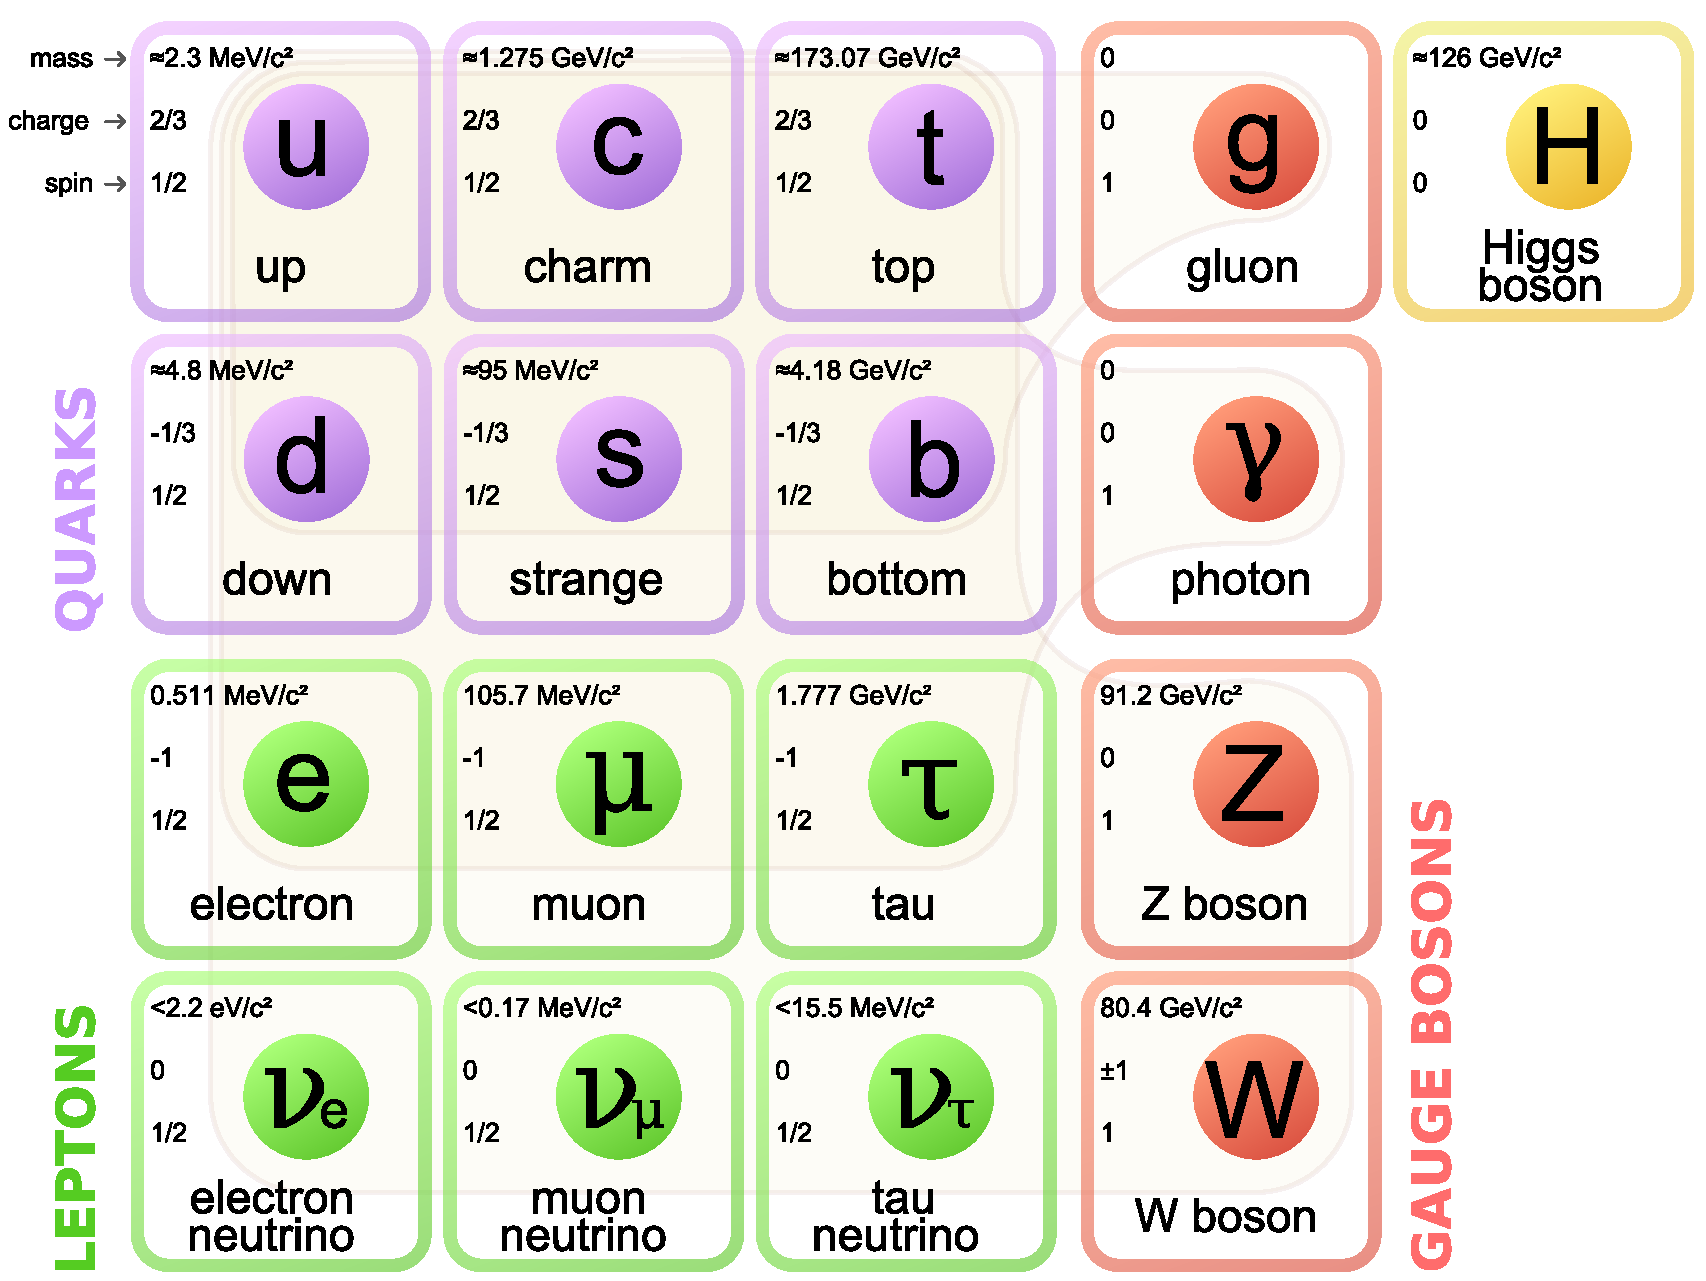
\includegraphics[width=0.95\textwidth]{figures/Standard_Model_of_Elementary_Particles.pdf}
\caption{A table of all the elementary particles in the standard model, with the spin, electric charge, and mass values of each particle \cite{MissMJ}. The faint gray lines indicate which gauge bosons interact with which fermions.}
\label{fig:sm-particles}
\end{center}
\end{figure}

The electromagnetic force is mediated by photons ($\gamma$), spin-1 gauge bosons which have no mass or electric charge $Q$. This force causes interactions between electrically charged particles and has infinite range due to the masslessness of the photon. Quantum electrodynamics (QED) is the quantum field theory description of electromagnetism, which can be represented by a $U(1)$ symmetry group. The weak force is mediated by the massive \Wpm and \Z bosons and can be represented by an $SU(2)$ symmetry group. The weak force acts on particles carrying weak isospin $T$. Weak isospin is a quantum number whose third component $T_3$ is conserved in all interactions and which can be mathematically treated in the same way as angular momentum, though the two quantities are physically distinct. The massiveness of the weak carrier bosons means that the weak force has a limited range, approximately $10^{-18}\unit{m}$. The charged current weak interaction, mediated by the \Wpm bosons, is sensitive to the chirality of fermions; only left-handed fermions and right-handed antifermions participate in this interaction. The neutral current weak interaction, mediated by the \Z boson, is not sensitive to chirality.

As suggested by the inclusion of both forces in the previous paragraph, the electromagnetic and weak forces can be unified to form the electroweak force, represented by the symmetry group $SU(2) \times U(1)$. In this unification, the quantum numbers of electromagnetism and the weak force are related by a new conserved quantum number, weak hypercharge $Y = 2(Q - T_3)$. The Higgs mechanism is responsible for electroweak symmetry breaking (EWSB). In order for the electroweak theory to be gauge invariant, the gauge bosons must be massless, but the \Wpm and \Z bosons are observed to have mass. The Higgs mechanism solves this dilemma via spontaneous EWSB due to its non-zero vacuum expectation value (VEV). The Higgs field consists of a doublet, with two charged particles and two neutral particles, all scalar bosons. The two charged particles and one of the neutral particles act as Goldstone bosons, combining with the \Wpm and \Z bosons to produce their masses. The remaining neutral particle is the Higgs boson, which was discovered at the LHC in 2012 \cite{NewBoson}.

The strong force, quantum chromodynamics (QCD), is mediated by gluons (\cPg) and can be represented by an $SU(3)$ symmetry group. Gluons, like photons, are spin-1 gauge bosons without mass or electric charge. However, gluons do possess color charge, the quantum number on which the strong force acts. Color charge is so named because the charge has three possible values, which are labeled red, green, or blue. Because gluons both mediate and participate in the strong interaction, the force between quarks does not decrease as they become spatially separated. The energy in the gluon field between the separated quarks can become large enough to form one or more quark-antiquark pairs. This phenomenon is known as confinement and prevents quarks or gluons from existing in a bare state. Correspondingly, the range of the strong force is limited to ${\sim} 10^{-15}\unit{m}$. Bound states of quarks and gluons, the only way they have ever been observed in nature, are called hadrons, and the formation of those bound states is called hadronization. States with one quark and one antiquark are mesons, while states with three quarks are baryons. Mesons and baryons are the two allowed types of bound states because they represent color singlets. Complementarily, as quarks get closer together, the strong force between them weakens. This behavior is known as asymptotic freedom; because short distances are equivalent to high energies, the strong interactions of quarks at a high-energy collider like the LHC can be calculated perturbatively. A residual form of the strong force acts on nucleons, protons and neutrons, to form atomic nuclei.

As mentioned, fermions are the particles of matter, which are separated into two groups: quarks and leptons. Quarks have fractional electric charge, weak isospin, and color charge, so they are affected by all three fundamental forces. There are two types of quarks: up-type quarks that have $Q = 2/3$ and down-type quarks that have $Q = -1/3$. Leptons consist of charged leptons and neutrinos. Charged leptons possess electric charge and weak isospin, while neutrinos only possess weak isospin. Three generations exist for each type of particle, with the different particles called flavors. The flavors of up-type quarks are the up, charm, and top quarks; of down-type quarks are the down, strange, and bottom quarks; of charged leptons are the electron, muon, and tau lepton; and of the neutrinos are the electron, muon, and tau neutrinos. The charged current weak interaction mixes the different flavors of quarks, with the amount of mixing between any two flavors given by the unitary Cabibbo-Kobayashi-Maskawa (CKM) matrix. The top quark is the heaviest elementary particle and is so heavy that it decays before hadronizing, making it an exception to the rule that bare quarks are not observed. Quarks possess an additively conserved quantum number called baryon number $B$, which is defined as $B = \frac{1}{3}(n_{\cPq} - n_{\overline{\cPq}})$. Similarly, lepton number $L$ is defined for leptons as $L = n_{\ell} - n_{\overline{\ell}}$. Specific lepton flavor numbers $L_{\Pe}$, $L_{\mu}$, $L_{\tau}$ are defined for each flavor pair of leptons.

The fermions are arranged into multiplets based on their chirality. The left-handed up- and down-type quarks are grouped together in a doublet $\cPq_L$, as are the left-handed charged leptons and neutrinos in $\ell_L$. The right-handed particles are singlets. It is important to note that right-handed neutrinos, and correspondingly left-handed antineutrinos, do not exist in the standard model. The Higgs field spontaneously provides masses to the quarks and charged leptons through a Yukawa interaction which couples the left- and right-handed versions of each flavor of particle. For a fermion $f$, this interaction takes the form $-y_{f} \overline{f}_{L} \PH f_{R}$, where $y_{f}$ is the Yukawa coupling. The quantum numbers of each type of particle are summarized in Table \ref{tab:q-num}, and the interactions among all the particles are illustrated in Fig. \ref{fig:sm-interactions}.

\begin{table}[htb]
  \begin{center}
%    \def\arraystretch{2.0} %1 is the default
    \begin{tabular}{|l||l|r|r|r|r|r|}
\hline
      & \multicolumn{1}{c|}{Particle} & \multicolumn{1}{c|}{$Q$} & \multicolumn{1}{c|}{$T_3$} & \multicolumn{1}{c|}{$Y$} & \multicolumn{1}{c|}{$B$} & \multicolumn{1}{c|}{$L$} \\
\hline
\hline
\multirow{3}{*}{Quarks}  
\rule{0pt}{24pt}         & $\cPq_L = \doublet[r]{\cPqu}{\cPqd}_L$ & $\doublet[r]{2/3}{-1/3}$ & $\doublet[r]{1/2}{-1/2}$ & $1/3$  & $1/3$ & 0 \\
                         & $\cPqu_R$                              & $2/3\hphantom{\bigg)}$   & $0\hphantom{\bigg)}$     & $4/3$  & $1/3$ & 0 \\
                         & $\cPqd_R$                              & $-1/3\hphantom{\bigg)}$  & $0\hphantom{\bigg)}$     & $-2/3$ & $1/3$ & 0 \\
\hline
\hline
\multirow{2}{*}{Leptons} 
\rule{0pt}{24pt}         & $\ell_L = \doublet[r]{\nu}{\Pe}_L$     & $\doublet[r]{0}{-1}$     & $\doublet[r]{1/2}{-1/2}$ & $-1$   & 0     & 1 \\
                         & $\Pe_R$                                & $-1\hphantom{\bigg)}$    & $0\hphantom{\bigg)}$     & $-2$   & 0     & 1 \\
\hline
    \end{tabular}
    \caption{The quantum numbers of each category of fermions, based on chirality and particle type: up-type quarks, down-type quarks, charged leptons, and neutrinos. The various flavors of each category, also called the first, second, and third generations of matter, possess the same quantum numbers and differ only in their masses.}
    \label{tab:q-num}
  \end{center}
\end{table}

\begin{figure}[hbt]
\begin{center}
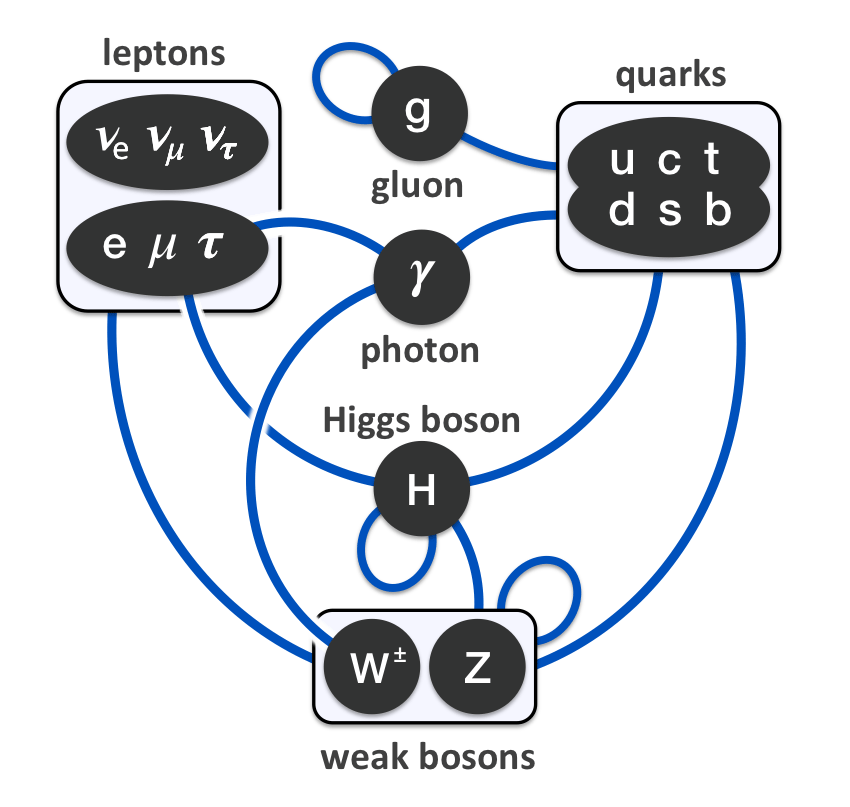
\includegraphics[width=0.95\textwidth]{figures/Elementary_particle_interactions_in_the_Standard_Model.png}
\caption{A diagram illustrating the leading order interactions between particles in the standard model, including self-interactions \cite{Drexler}.}
\label{fig:sm-interactions}
\end{center}
\end{figure}

%\addtocounter{section}{-1}
\renewcommand{\thesection}{\thechapter.{$\frac{1}{2}$}}
\section{Beyond the Standard Model}
\newcounter{sectionprime}
\addtocounter{sectionprime}{\value{section}}
\addtocounter{sectionprime}{-1}
\renewcommand{\thesection}{\thechapter.\arabic{sectionprime}} % use offset numbering

The predictions of the standard model have been confirmed by decades of precise experimental tests. However, as an effective field theory, its domain of applicability is ultimately limited; at a high enough energy, the theory will break down. Further, the standard model is unable to account for some observations. These limitations and indications of new phenomena motivate various searches for physics beyond the standard model (BSM), include the searches which will be presented in this dissertation.

The most obvious limitation of the standard model is that it depends on 19 free parameters which must be determined by experiment. These parameters include the nine fermion masses, the Higgs mass and VEV, the gauge couplings for the three forces, the three mixing angles and one phase from the CKM matrix, and finally the QCD vacuum angle. It is conceivable that a BSM theory could reduce the number of free parameters. Electroweak unification and charge quantization suggest that a Grand Unified Theory (GUT) could unify all three fundamental forces, at an expected energy scale of ${\sim} 10^{16}\GeV$. The observation of neutrino oscillations is now well established, indicating that neutrinos have small but non-zero masses. The oscillation of neutrinos between mass and flavor eigenstates is described by the Pontecorvo-Maki-Nakagawa-Sakata (PMNS) matrix. Like the CKM matrix for quarks, the PMNS matrix is unitary and has four parameters: three mixing angles and one phase. The values of the neutrino masses have not been directly measured, but are indirectly limited to the \eVns scale. Because right-handed neutrinos do not exist in the Standard Model, neutrinos cannot gain mass via a Yukawa interaction with the Higgs field. Though the Higgs mass is a parameter of the SM, it can be calculated in many BSM theories. Unless unnatural fine-tuning occurs, the presence of new massive particles makes this calculation produce a value near the Planck scale of $10^{19}\GeV$, orders of magnitude higher than the observed value of 125\GeV, which characterizes the electroweak scale. This is known as the hierarchy problem. To construct a natural theory which avoids such fine-tuning while making predictions that agree with observation, it is necessary to cancel divergent contributions to the Higgs mass. The hierarchy problem is an important motivation to search for new physics at the LHC \cite{Morrissey20121}.

Astrophysics provides numerous indications of the need for BSM theories. Most notably, gravity is not included in the standard model. A successful unification of general relativity and quantum field theory has not been achieved, due to the difficulty of constructing a renormalizable theory for the spin-2 graviton. At the Planck scale, gravitational effects become comparable to SM interactions, which calls for a new theory. The measurement of galactic rotation curves and galaxy cluster collisions \cite{BulletCluster} indicates that ${\sim} 85\%$ of the matter in the universe is dark matter, which interacts gravitationally but not electromagnetically. Dark matter is likely to be a new particle not present in the standard model. The most popular type of dark matter candidate is a weakly interacting massive particle (WIMP) \cite{Morrissey20121}, but many other candidates have been proposed. The dearth of antimatter relative to the amount of matter in the universe requires greater violation of charge-parity (CP) symmetry than is contained in the SM. The accelerating expansion of the universe, observed using standard candle supernovae \cite{Supernova98,Supernova99}, implies that ${\sim} 70\%$ of the energy of the universe exists in a unknown form called dark energy. Dark energy may be a result of the cosmological constant of the universe, which can be related to the energy of the vacuum in quantum field theory. However, the standard model predicts that this cosmological constant would be $10^{120}$ times larger than the observed value, a clear failure of the theory. The recent tentative evidence for cosmic inflation from the Background Imaging of Cosmic Extragalactic Polarization (BICEP) experiment \cite{BICEP} implies the existence of the inflaton, a new scalar field.

The following sections discuss the theories of leptoquarks and R-parity violating supersymmetry. The existence of leptoquarks can be a consequence of grand unification or other theories that address the parallels between leptons and quarks in the standard model. Supersymmetry is motivated by basic considerations of quantum field theory, the hierarchy problem, grand unification, and dark matter. The introduction of R-parity violation in supersymmetry evades existing limits on signatures with large missing transverse energy due to the stability of the lightest supersymmetric particle, while retaining some of the other desirable characteristics of supersymmetry. R-parity violating supersymmetry can also act as a signature generator to suggest novel searches which might discover or rule out other BSM theories \cite{EvansSigGen}.

\stepcounter{sectionprime}
\section{Leptoquarks
\label{sec:LQ}}

Many BSM theories include a deeper relationship between leptons and quarks. Such a relationship is indicated by the cancellation of SM gauge anomalies from triangle diagrams, which requires each generation of matter to consist of quarks and leptons with the specific weak hypercharge values and multiplet arrangements that they possess in the SM \cite{Peskin}. Such theories introduce a class of particles called leptoquarks (LQs), which possess lepton number, baryon number, color charge, and fractional electric charge. Leptoquarks are bosons, either scalar with spin 0 or vector with spin 1. The values of the LQ quantum numbers, including those listed previously as well as weak isospin, which they may or may not possess, are model-dependent. A total fermion number $F$ can be defined as $F = 3B + L$ to characterize the combinations of lepton and baryon numbers found in LQs. The possible values are $F=0$ for LQs which couple to $\overline{\ell}\cPq$ or $\ell\overline{\cPq}$ pairs and $|F|=2$ for coupling to $\ell\cPq$ or $\overline{\ell}\overline{\cPq}$ pairs.

The first BSM theory to include leptoquarks was Pati-Salam $SU(4)$ \cite{SU4}, a GUT which casts lepton number as the fourth type of color charge, hence the $SU(4)$ symmetry instead of the SM $SU(3)$. Another GUT, Georgi-Glashow $SU(5)$ \cite{GUT}, also contains leptoquarks. In general, grand unified theories group leptons and quarks together in multiplets. However, the symmetry breaking in these theories typically occurs at the GUT scale, rendering the expected LQ masses very large and therefore unable to be directly produced at colliders. $E_6$ superstring theory \cite{SUPERSTR} can also contain LQs, as it behaves similarly to GUTs below the string compactification scale, which is typically near the Planck scale. In other models, leptoquarks may be composite particles \cite{LQ3b}. These include extended technicolor theories \cite{TC3}, which postulate a new strong interaction similar to QCD and provide spontaneous masses to SM fermions using technifermions. A techniquark and anti-technilepton can bind together to form a technimeson which interacts with SM fermions as a leptoquark with a model-dependent coupling. Technicolor, though, has become disfavored with the confirmation of the Higgs mechanism for EWSB and fermion masses.

The Buchm\"{u}ller-R\"{u}ckl-Wyler (BRW) model of leptoquarks includes all renormalizable Lagrangian terms compatible with the standard model \cite{BRW}. There are several constraints imposed in the BRW model:
\begin{enumerate}
\item LQ interactions are dimensionless, in order to be renormalizable.
\item LQ interactions are invariant under the overall SM symmetry $SU(3) \times SU(2) \times U(1)$.
\item LQ interactions conserve $B$ and $L$, to avoid contributions to proton decay.
\item LQs couple only to SM particles.
\end{enumerate}
Further consideration of experimental limits imposes two additional constraints, creating the minimal BRW (mBRW) model:
\begin{enumerate}
\setcounter{enumi}{4}
\item LQ couplings are chiral, involving either only left-handed fermions or only right-handed fermions, due to limits on otherwise chirally-suppressed decays such as $\pi^{+} \rightarrow \Pe^{+} \nu_{\Pe}$.
\item LQ couplings involve only a single generation of leptons and quarks, to evade limits on flavor-changing neutral currents (FCNCs).
\end{enumerate}
The Lagrangian terms are given for scalar LQs in Eq. \eqref{eq:Lagrangian-SLQ} and for vector LQs in Eq. \eqref{eq:Lagrangian-VLQ} below, using the ``Aachen'' notation as specified in Ref. \cite{ModelIndLQ}.
\begin{align}
\label{eq:Lagrangian-SLQ}
\mathcal{L}_{S} = &\hphantom{+~}(\lambda_{L,S_{0}} \overline{\cPq}_{L}^{c} i\sigma_{2} \ell_{L} + \lambda_{R,S_{0}} \overline{\cPqu}_{R}^{c} \Pe_{R})S_{0}^{\dagger}
+ \lambda_{R,\widetilde{S}_{0}} \overline{\cPqd}_{R}^{c} \Pe_{R} \widetilde{S}_{0}^{\dagger} \nonumber \\
&+ (\lambda_{L,S_{1/2}} \overline{\cPqu}_{R} \ell_{L} + \lambda_{R,S_{1/2}} \overline{\cPq}_{L} i\sigma_{2} \Pe_{R})S_{1/2}^{\dagger}
+ \lambda_{L,\widetilde{S}_{1/2}} \overline{\cPqd}_{R} \ell_{L} \widetilde{S}_{1/2}^{\dagger} \nonumber \\
&+ \lambda_{L,S_{1}} \overline{\cPq}_{L}^{c} i\sigma_{2}\boldsymbol{\sigma} \ell_{L} \cdot \boldsymbol{S}_{1}^{\dagger} + \text{h.c.} \\
%\end{align}
%\begin{align}
\label{eq:Lagrangian-VLQ}
\mathcal{L}_{V} = &\hphantom{+~}(\lambda_{L,V_{0}} \overline{\cPq}_{L} \gamma_{\mu} \ell_{L} + \lambda_{R,V_{0}} \overline{\cPqd}_{R} \gamma_{\mu} \Pe_{R})V_{0}^{\mu\dagger}
+ \lambda_{R,\widetilde{V}_{0}} \overline{\cPqu}_{R} \gamma_{\mu} \Pe_{R} \widetilde{V}_{0}^{\mu\dagger} \nonumber \\
&+ (\lambda_{L,V_{1/2}} \overline{\cPqd}_{R}^{c} \gamma_{\mu} \ell_{L} + \lambda_{R,V_{1/2}} \overline{\cPq}_{L}^{c} \gamma_{\mu} \Pe_{R})V_{1/2}^{\mu\dagger}
+ \lambda_{L,\widetilde{V}_{1/2}} \overline{\cPqu}_{R}^{c} \gamma_{\mu} \ell_{L} \widetilde{V}_{1/2}^{\mu\dagger} \nonumber \\
&+ \lambda_{L,V_{1}} \overline{\cPq}_{L} \gamma_{\mu}\boldsymbol{\sigma} \ell_{L} \cdot \boldsymbol{V}_{1}^{\mu\dagger} + \text{h.c.}
\end{align}
In these equations, scalar leptoquarks are denoted by $S$ and vector leptoquarks are denoted by $V$. The subscripts 0, 1/2, and 1 denote singlet, doublet, and triplet states, respectively. The $\widetilde{S}$ and $\widetilde{V}$ leptoquarks have different quantum numbers compared to the corresponding $S$ and $V$ leptoquarks. The coupling constants for the Yukawa couplings between leptoquarks, leptons, and quarks are represented by $\lambda$, with the chirality $L$ or $R$ and the leptoquark type indicated in the subscript. The generation indices for the couplings and fermion multiplets are suppressed. The Pauli matrices are denoted by $\sigma_{i}$ and the Dirac matrices by $\gamma_{\mu}$. The Hermitian conjugate terms are indicated as ``h.c.'' The quantum numbers for the different types of mBRW leptoquarks are listed in Table \ref{tab:lq-num}.

\begin{table}[htb]
  \begin{center}
%    \def\arraystretch{3.0} %1 is the default
    \begin{tabular}{|l||l|r|r|r|r|}
\hline
      & \multicolumn{1}{c|}{Particle} & \multicolumn{1}{c|}{$Q$} & \multicolumn{1}{c|}{$T_3$} & \multicolumn{1}{c|}{$Y$} & \multicolumn{1}{c|}{$F$} \\
\hline
\hline
\multirow{10}{*}{Scalar} & $S_{0}$               & $-1/3\hphantom{\bigg)}$                            & $0\hphantom{\bigg)}$                              & $-2/3$ & $2$ \\
                         & $\widetilde{S}_{0}$   & $-4/3\hphantom{\bigg)}$                            & $0\hphantom{\bigg)}$                              & $-8/3$ & $2$ \\
\rule{0pt}{24pt}         & $S_{1/2}$             & $\doublet[r]{-2/3}{-5/3}$ & $\doublet[r]{1/2}{-1/2}$ & $-7/3$ & $0$ \\
\rule{0pt}{24pt}         & $\widetilde{S}_{1/2}$ & $\doublet[r]{1/3}{-2/3}$  & $\doublet[r]{1/2}{-1/2}$ & $-1/3$ & $0$ \\
\rule{0pt}{36pt}         & $S_{1}$               & $\triplet[r]{2/3}{-1/3}{-4/3}$       & $\triplet[r]{1\vphantom{/}}{0\vphantom{/}}{-1\vphantom{/}}$             & $-2/3$ & $2$ \\
\hline
\hline
\multirow{10}{*}{Vector} & $V_{0}$               & $-2/3\hphantom{\bigg)}$                            & $0\hphantom{\bigg)}$                              & $-4/3$  & $0$ \\
                         & $\widetilde{V}_{0}$   & $-5/3\hphantom{\bigg)}$                            & $0\hphantom{\bigg)}$                              & $-10/3$ & $0$ \\
\rule{0pt}{24pt}         & $V_{1/2}$             & $\doublet[r]{-1/3}{-4/3}$ & $\doublet[r]{1/2}{-1/2}$ & $-5/3$  & $2$ \\
\rule{0pt}{24pt}         & $\widetilde{V}_{1/2}$ & $\doublet[r]{2/3}{-1/3}$  & $\doublet[r]{1/2}{-1/2}$ & $1/3$   & $2$ \\
\rule{0pt}{36pt}         & $V_{1}$               & $\triplet[r]{1/3}{-2/3}{-5/3}$       & $\triplet[r]{1\vphantom{/}}{0\vphantom{/}}{-1\vphantom{/}}$             & $-4/3$  & $0$ \\
\hline
    \end{tabular}
    \caption{The quantum numbers of the different types of scalar and vector leptoquarks in the mBRW model.}
    \label{tab:lq-num}
  \end{center}
\end{table}

As color-charged particles, leptoquarks are primarily produced by strong interactions in $\Pp\Pp$ collisions. For pair production of leptoquarks, these interactions include gluon-gluon fusion and quark-antiquark annihilation, whose LO forms are shown in Fig. \ref{fig:lq-diagrams}. An additional contribution to quark-antiquark annihilation may proceed through the Yukawa coupling $\lambda$ of the leptoquark to the quark and lepton pair. However, the ratio $\MLQ/\lambda$, where $\MLQ$ is the leptoquark mass, is restricted by limits from low-energy processes including $\pi^{+} \rightarrow \Pe^{+} \nu_{\Pe}$ and atomic parity violation. The limits on $\MLQ/\lambda$ range from 1800--6400\GeVcc, depending on the type of leptoquark \cite{Leurer:1993em, MuchAdo, LQreview}. The expected accessible mass range for leptoquarks at the LHC with $\sqrt{s}=14\TeV$ ranges from 900--1200\GeVcc for scalar LQs and 1200--1500\GeVcc for vector LQs, depending on the desired number of events \cite{LQPairHad}. Up to these masses, $\lambda$ will be small enough that its contribution to leptoquark production can be neglected. This applies both to the Yukawa-based pair production diagram in Fig. \ref{fig:lq-diagrams} and the single production diagrams from quark-gluon scattering in Fig. \ref{fig:lq-single}.

\begin{figure}[hbt]
\begin{center}
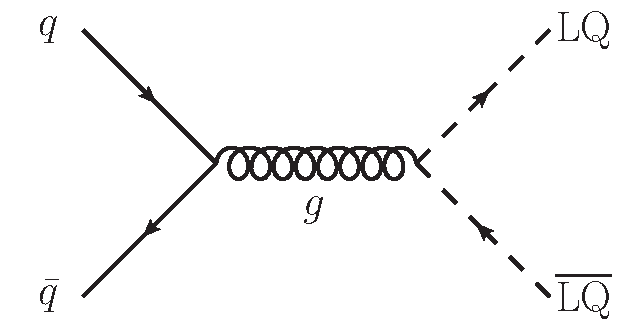
\includegraphics[width=0.49\textwidth]{figures/LO_FD_LQ_pair_a.pdf}
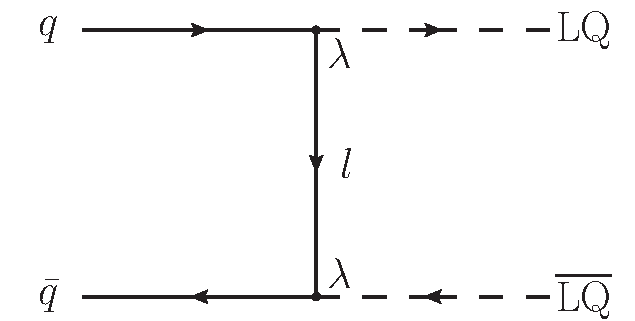
\includegraphics[width=0.49\textwidth]{figures/LO_FD_LQ_pair_b.pdf}
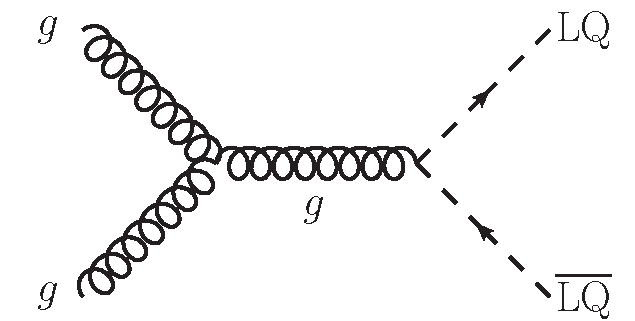
\includegraphics[width=0.49\textwidth]{figures/LO_FD_LQ_pair_c.pdf}
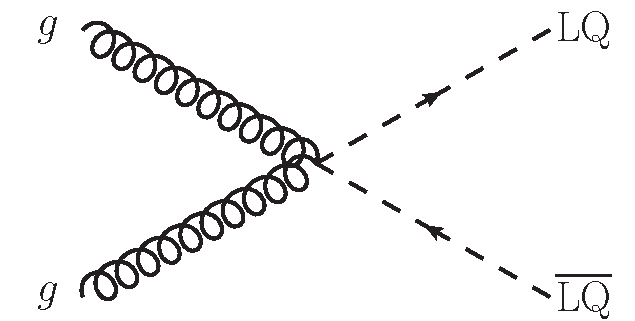
\includegraphics[width=0.49\textwidth]{figures/LO_FD_LQ_pair_d.pdf}
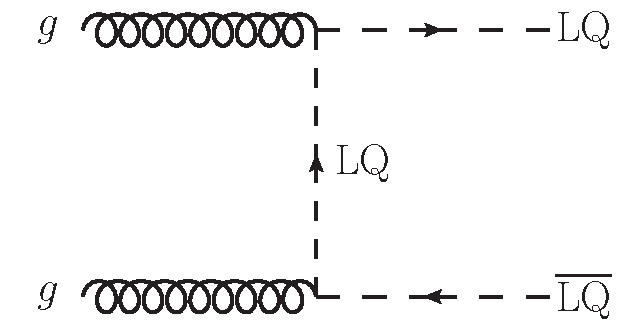
\includegraphics[width=0.49\textwidth]{figures/LO_FD_LQ_pair_e.pdf}
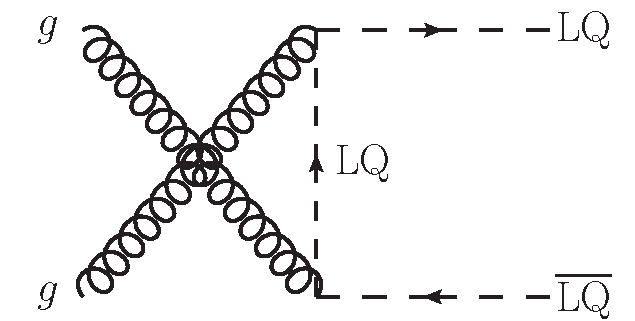
\includegraphics[width=0.49\textwidth]{figures/LO_FD_LQ_pair_f.pdf}
\caption{The LO diagrams for leptoquark pair production from quark-antiquark annihilation (top) and gluon-gluon fusion (middle, bottom).}
\label{fig:lq-diagrams}
\end{center}
\end{figure}

\begin{figure}[hbt]
\begin{center}
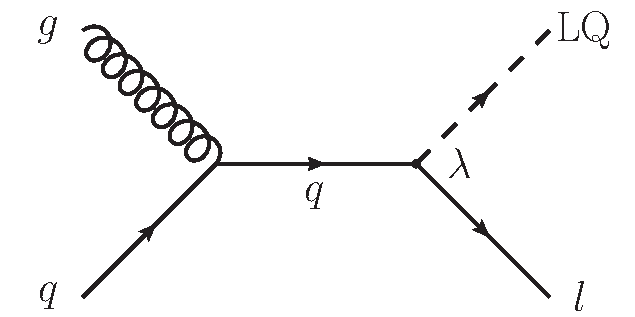
\includegraphics[width=0.49\textwidth]{figures/LO_FD_single_LQ_a.pdf}
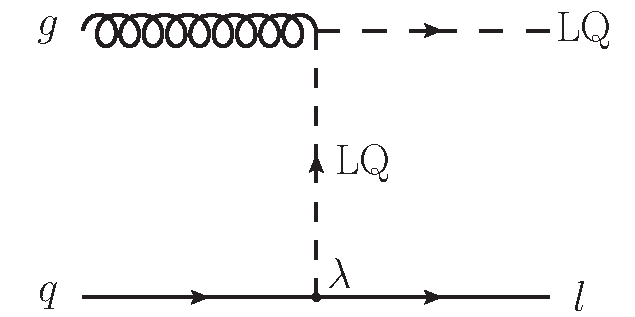
\includegraphics[width=0.49\textwidth]{figures/LO_FD_single_LQ_b.pdf}
\caption{The LO diagrams for single leptoquark production from quark-gluon scattering. The LQ is produced in association with a lepton.}
\label{fig:lq-single}
\end{center}
\end{figure}

Table \ref{tab:lq-xsec} lists the pair production cross sections for a range of scalar leptoquark masses. They have been calculated using the CTEQ6 parton distribution functions (PDFs) \cite{CTEQ6r1,CTEQ6r2} with $K$-factors applied to include NLO corrections from QCD \cite{LQxsec}. Theoretical uncertainties are calculated by propagating the PDF uncertainty and varying the factorization/renormalization scale $\mu$. These cross sections are sensitive only to the leptoquark mass and spin, so they are largely model-independent. For vector leptoquarks, the cross sections may be modified by anomalous triple and quartic gauge couplings. The decay widths for scalar and vector leptoquarks can be calculated according to Eqs. \eqref{eq:SLQ-width} and \eqref{eq:VLQ-width}, respectively \cite{BRW}:
\begin{align}
\label{eq:SLQ-width} \Gamma_{S} &= \sum_{i}{\frac{\lambda_{i}^{2}}{16\pi}\MLQ}, \\
\label{eq:VLQ-width} \Gamma_{V} &= \sum_{i}{\frac{\lambda_{i}^{2}}{24\pi}\MLQ}.
\end{align}
Equations \eqref{eq:SLQ-width} and \eqref{eq:VLQ-width} sum over all Yukawa couplings for a given leptoquark. Given the limits on $\lambda$ discussed above, leptoquarks accessible at the LHC with a single Yukawa coupling can be expected to have a fractional decay width of less than 0.1--0.2\%.

\begin{table}[htb]
\begin{center}
{\footnotesize
\begin{tabular}{|l||c|c||c|c|}
\hline
$\MLQ$ & $\sigma (\mu = \MLQ)$ & $\delta (\text{PDF}) $ & $\sigma (\mu = \MLQ/2)$ & $\sigma (\mu = 2\MLQ)$ \\
\hline
\hline
 200 & 17.4 & 1.24 & 15.0 & 19.7  \\
 250 & 5.26 & 0.487 & 4.54 & 5.94  \\
 300 & 1.89 & 0.214 & 1.63 & 2.13  \\
 350 & 0.77 & 0.102 & 0.663 & 0.866  \\
 400 & 0.342 & 0.052 & 0.295 & 0.385  \\
 450 & 0.163 & 0.0278 & 0.14 & 0.183  \\
 500 & 0.082 & 0.0155 & 0.0704 & 0.0922  \\
 550 & 0.0431 & 0.00893 & 0.037 & 0.0485  \\
 600 & 0.0235 & 0.0053 & 0.0201 & 0.0265  \\
 650 & 0.0132 & 0.00322 & 0.0113 & 0.0149  \\
 700 & 0.00761 & 0.002 & 0.00648 & 0.00858  \\
 750 & 0.00448 & 0.00126 & 0.00381 & 0.00506  \\
 800 & 0.00269 & 0.00081 & 0.00228 & 0.00304  \\
 850 & 0.00164 & 0.000527 & 0.00139 & 0.00186  \\
 900 & 0.00101 & 0.000347 & 0.000856 & 0.00115  \\
 950 & 0.000634 & 0.000231 & 0.000534 & 0.000722  \\
 1000 & 0.000401 & 0.000155 & 0.000337 & 0.000458  \\
\hline
\end{tabular}
}
\caption{The pair production cross sections for a range of scalar leptoquark masses at $\sqrt{s}=8\TeV$. Theoretical uncertainties from the PDFs and from varying the factorization/renormalization scale $\mu$ from $\mu=\MLQ/2$ to $\mu=2\MLQ$ are indicated.}
\label{tab:lq-xsec}
\end{center}
\end{table}

In this dissertation, a search is performed for pair production of scalar leptoquarks decaying to third generation fermions. The symbol $\mathcal{B}$ is used for the branching fraction for the decay $\text{LQ} \rightarrow \tau \cPqb$. This results a final state with two tau leptons and two bottom quarks. One tau lepton is required to decay leptonically: $\tau \rightarrow \ell \overline{\nu_{\ell}} \nu_{\tau}$, where $\ell$ can be a muon or an electron, which are collectively called light leptons. The other tau lepton is required to decay hadronically, denoted as \tauh; see Sec. \ref{sec:hpstau} for more information about hadronic decays of tau leptons. These decays result in two channels based on the leptonic decay of the tau, which are labeled as \etau and \mutau, or collectively \ltau when the light lepton flavor is unimportant. Both bottom quarks hadronize into b-jets, as described in Sec. \ref{sec:b-tagging}. Currently, the strongest mass limits on such third-generation scalar leptoquarks come from direct searches. Assuming $\mathcal{B}=100\%$, the lower limit is approximately 530\GeV, set by both the CMS \cite{CMSLQ3} and ATLAS \cite{ATLASLQ3} experiments using 4.7--4.8\fbinv of data from $\Pp\Pp$ collisions with $\sqrt{s}=7\TeV$. Indirect limits from low-energy processes are discussed in Refs. \cite{ModelIndLQ,Leurer:1993em, MuchAdo, LQreview}.

%talk about reinterpreted search to cover low B?

\stepcounter{sectionprime}
\section{R-Parity Violating Supersymmetry
\label{sec:RPVSUSY}}

At the most basic level, supersymmetry proposes a symmetry between bosons and fermions. Such a symmetry appeals to mathematical considerations in quantum field theory by simplifying many calculations \cite{Peskin}. However, the primary motivation for a theory of SUSY with effects at the electroweak scale and therefore accessible at the LHC is the hierarchy problem. The mass of the Higgs boson, experimentally measured as $M_{\PH} = 125\GeV$, is theoretically sensitive to quantum corrections via loop diagrams from any particle that couples to it. This sensitivity makes the experimentally-measured value highly suspicious. Precise cancellations must occur among the various quantum corrections to produce such a small mass value, relative to the expected energy scales of new physics. Any BSM theory lacking a simple mechanism to produce such cancellations must undergo unnatural fine-tuning in order to arrive at the correct value of $M_{\PH}$. The following discussion of supersymmetry is drawn primarily from Ref. \cite{Primer}.

The Higgs mass parameter $m_{\PH}^{2}$ appears in the Higgs potential:
\begin{equation}
V = m_{\PH}^{2}|\PH|^{2} + \lambda_{\PH}|\PH|^{4}.
\end{equation}
Consider the one-loop contribution to $m_{\PH}^{2}$ from a fermion $f$ which has a Yukawa coupling to the Higgs field, $-y_{f} \overline{f}_{L} \PH f_{R}$. The correction term in the mass parameter calculation can be written as follows:
\begin{equation}
\Delta_{f} m_{\PH}^{2} = -\frac{|y_{f}|^{2}}{8\pi^{2}}\Lambda_{\text{UV}}^{2} + \cdots. \label{eq:DMH-fermion}
\end{equation}
The factor $\Lambda_{\text{UV}}$ is the cutoff scale used to handle the ultraviolet divergence in the loop integral through regularization. This cutoff scale is typically related to the energy scale of new physics, e.g. the GUT scale or Planck scale. Even if the cutoff scale is small, the contribution to the Higgs mass from any new heavy fermion will be proportional to its Yukawa coupling $y$, which could itself be large. Similarly, consider the one-loop contribution from a scalar boson $S$ with a coupling to the Higgs written as $-y_{S} |\PH|^{2} |S|^{2}$, which produces a correction term:
\begin{equation}
\Delta_{S} m_{\PH}^{2} = \frac{y_{S}}{16\pi^{2}}\Lambda_{\text{UV}}^{2} + \cdots. \label{eq:DMH-scalar}
\end{equation}
Both one-loop diagrams are shown in Fig. \ref{fig:higgs-cancel}. The leading terms of Eqs. \eqref{eq:DMH-fermion} and \eqref{eq:DMH-scalar} have opposite signs, which suggests that the two terms could cancel if there were two scalars for each fermion, with $y_{S} = |y_{f}|^2$.

\begin{figure}[hbt]
\begin{center}
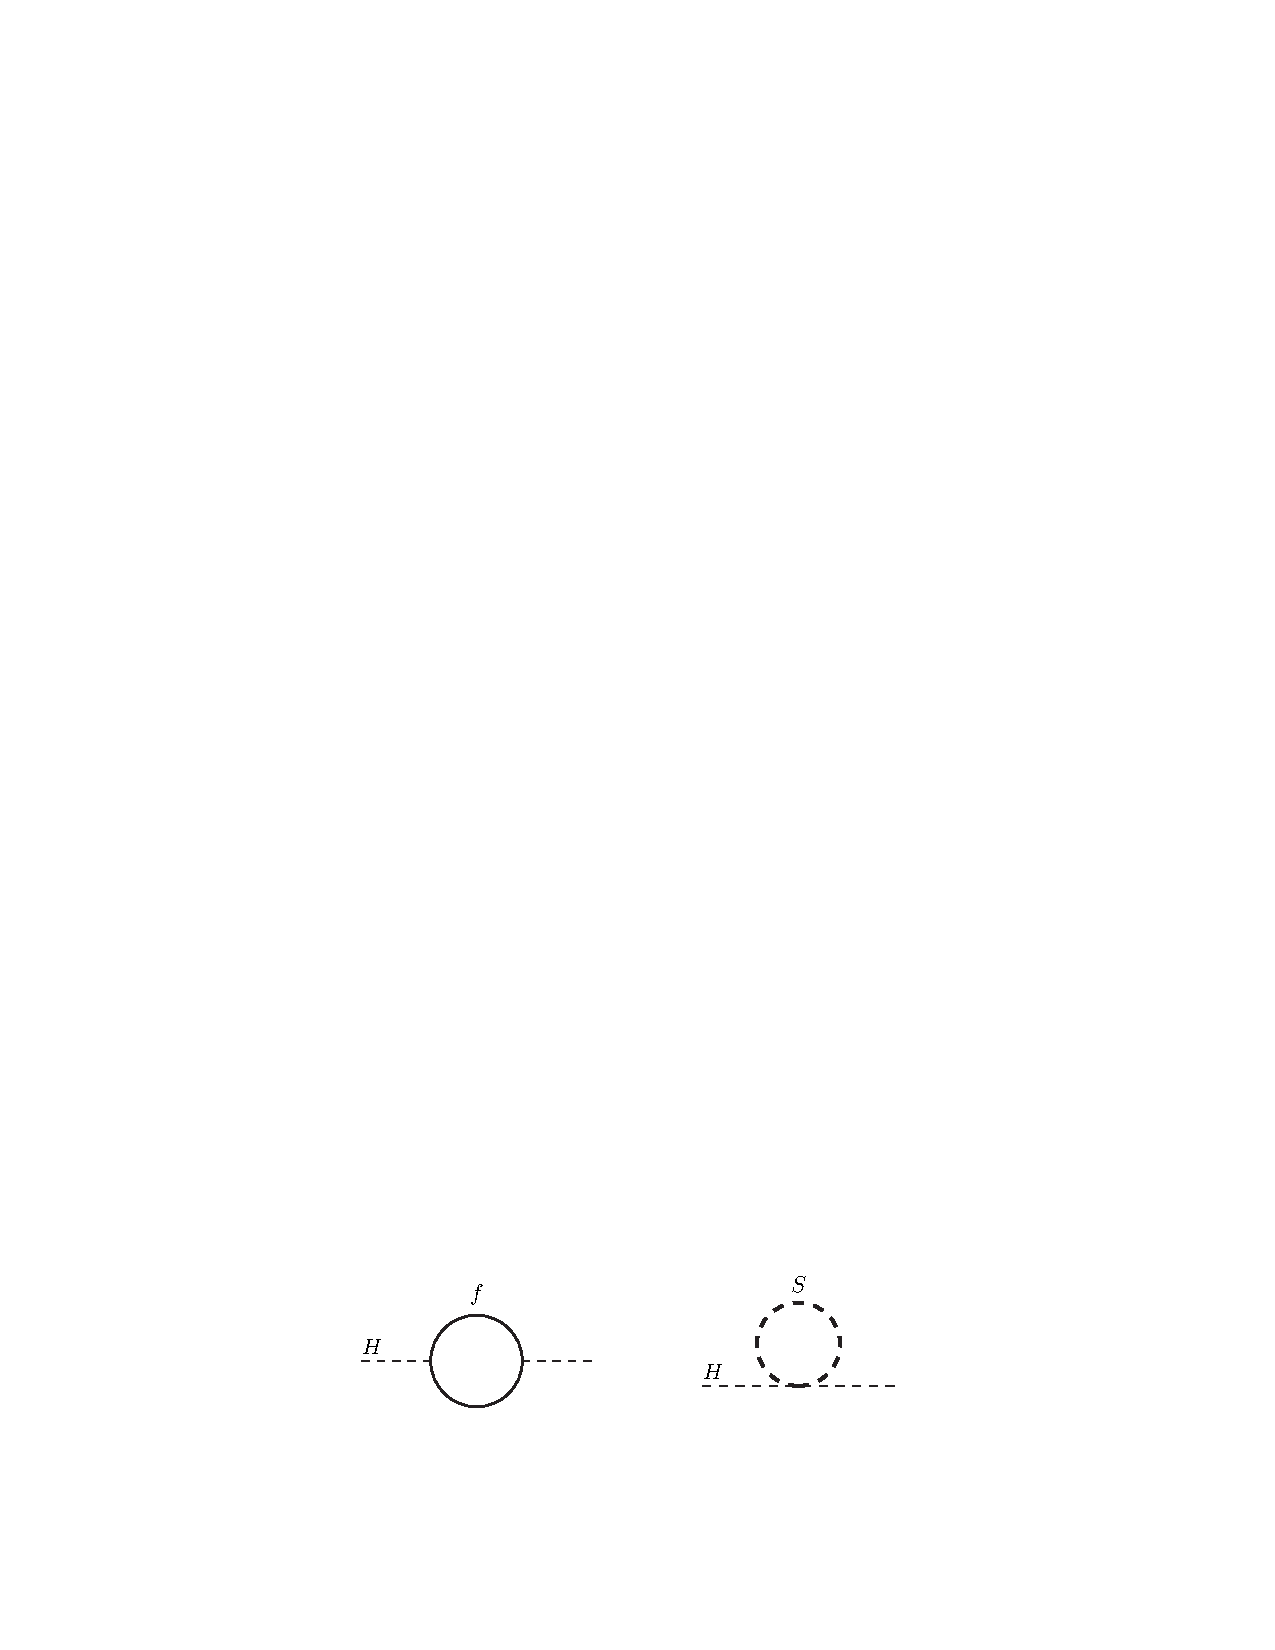
\includegraphics[width=0.95\textwidth]{figures/9709356v6-higgs-cancel.pdf}
\caption{One-loop diagrams for contributions to the Higgs mass parameter $m_{\PH}^{2}$ from a fermion $f$ (left) and a scalar $S$ (right) \cite{Primer}.}
\label{fig:higgs-cancel}
\end{center}
\end{figure}

This observation motivates SUSY as an extension of the standard model. While many formulations of SUSY exist, it is instructive to consider the minimal supersymmetric model (MSSM) to understand the fundamental components of the class of SUSY theories. SM particles are paired with new particles called superpartners with a spin difference of 1/2; SM fermions have scalar boson superpartners and SM bosons have spin-1/2 fermion superpartners. The scalar superpartners are named after the corresponding SM fermions with the prefix ``s-'', e.g. squarks and sleptons. The fermionic superpartners are named after the corresponding SM bosons with the suffix ``-ino'', e.g. higgsinos and gauginos. The symbols for superpartners are indicated by a tilde $\widetilde{\hphantom{H}}$. SM particles and their superpartners are arranged together in supermultiplets which extend the multiplets listed in Table \ref{tab:q-num}. Chiral supermultiplets contain scalar bosons and spin-1/2 fermions, while gauge supermultiplets contain spin-1/2 fermions and vector bosons. The superpartners possess the same quantum numbers as the corresponding SM particles, except for spin.

The Higgs boson, as a scalar, therefore becomes part of a chiral supermultiplet with weak hypercharge values $Y = \pm 1/2$. However, the existence of such chiral higgsinos creates new triangle gauge anomalies which must be cancelled to preserve the consistency of the theory. In addition, the weak hypercharge values of the Higgs supermultiplet restrict the possible Yukawa interactions with the other chiral supermultiplets, which are necessary for spontaneous fermion masses. For both of these reasons, the MSSM contains two Higgs doublets, conventionally labeled \Hone and \Htwo to indicate their couplings to up-type quarks or down-type quarks and charged leptons, respectively. Each Higgs doublet has its own VEV, labeled $v_{\cPqu}$ and $v_{\cPqd}$, which are considered to be two components of an underlying $v$, implying an angle $\beta$ can be defined as $\text{tan}(\beta) = v_{\cPqu}/v_{\cPqd}$.

Given these details, the superpotential of the MSSM, $W_{\text{MSSM}}$, contains these terms:
\begin{equation}
W_{\text{MSSM}} = y_{\cPqu,ij}\PU_{i}^{c}\PQ_{j}\Hone + y_{\cPqd,ij}\PD_{i}^{c}\PQ_{j}\Htwo + y_{\Pe,ij}\PE_{i}^{c}\PL_{j}\Htwo + \mu \Hone \Htwo. \label{eq:WMSSM}
\end{equation}
Equation \eqref{eq:WMSSM} is written in terms of superfields. $\PU$ is the up-type quark singlet superfield; $\PD$ is the down-type quark singlet superfield; $\PQ$ is the quark doublet superfield; $\PE$ is the charged lepton singlet superfield; and $\PL$ is the lepton doublet superfield. The Yukawa couplings $y$ are labeled by the fermion type $\cPqu$, $\cPqd$, or $\Pe$ with generation indices $i$, $j$. As an example, the top quark Yukawa coupling is $y_{\cPqu,33} = y_{\cPqt}$. The higgsino mass parameter is denoted as $\mu$.

The superpotential is limited to these terms by requiring the conservation of $R$-parity. The quantity $R$ is related to the baryon and lepton numbers as well as the particle spin $S$ and may be defined in two equivalent ways \cite{Barbier}, as shown in Eq. \eqref{eq:Rdef}. Equation \eqref{eq:Rparity} defines $R$-parity based on $R$.
\begin{align}
R &= 3B+L+2S = 3(B-L)+2S, \label{eq:Rdef} \\
R_{p} &= (-1)^{R}. \label{eq:Rparity}
\end{align}
All SM particles have $R_{p} = +1$, while all superpartners have $R_{p} = -1$. If $R$-parity is conserved, interactions which violate lepton or baryon number are not allowed. Notably, there must necessarily be a lightest supersymmetric particle (LSP) that is stable in order to conserve $R$-parity in the decay of any SUSY particle. In many models, the LSP is the lightest neutralino, a state created by mixing between the neutral higgsinos and gauginos due to EWSB. As a weakly interacting massive particle, the neutralino LSP is a promising candidate for WIMP dark matter.

If supersymmetry were unbroken, superpartners would have the same masses as their corresponding SM particles and would already have been detected. Therefore, there must be some mechanism responsible for breaking supersymmetry. In order for broken SUSY to continue to solve the hierarchy problem, it must preserve the conditions such as $y_{S} = |y_{f}|^2$ that lead to natural cancellations in the Higgs mass correction terms. So-called ``soft'' supersymmetry breaking accomplishes this by separating the Lagrangian into two separate terms:
\begin{equation}
\mathcal{L} = \mathcal{L}_{\text{SUSY}} + \mathcal{L}_{\text{soft}},
\end{equation}
where $\mathcal{L}_{\text{SUSY}}$ is made up of the SUSY-preserving terms, including the Yukawa interactions from the superpotential as well as the gauge interactions, and $\mathcal{L}_{\text{soft}}$ is made up of the SUSY-violating terms. The contributions to $\mathcal{L}_{\text{soft}}$ must be only mass terms and couplings whose parameters have positive mass dimension. These include interactions between three scalars, two sfermions and a Higgs, such as $a_{\cPqu,ij} \sUp_{i}^{c} \sQua_{j} \Hone$, where $a_{\cPqu,ij}$ are the soft couplings for those interactions. All such soft couplings are either at or below the mass scale $m_{\text{soft}}$, which is expected to be around the TeV scale from hierarchy problem considerations.

In general, the soft SUSY breaking terms can introduce FCNCs and CP violation that are strictly limited by precision measurements. This can be avoided by assuming the sfermion masses are universal; in other words, all sfermions should have the same mass regardless of flavor. This ``flavor-blindness'' eliminates mixing between flavors, and as a bonus, greatly reduces the number of free parameters in the MSSM. For first- and second-generation sfermions, flavor-blind universal masses are the norm. However, in the third generation, the sfermion masses can differ from the other two generations. In SUSY calculations, the couplings and mass parameters are treated as running factors which change based on renormalization group (RG) equations. These RG equations lead to corrections which tend to be small for Yukawa interactions, except for third generation particles which have relatively large Yukawa couplings. The effects of RG evolution in SUSY on the gauge couplings for the three fundamental forces significantly aid grand unification, which is another motivation for SUSY.

The concept of naturalness, described in Ref. \cite{NaturalSUSY}, indicates that the third-generation sfermion masses should in fact be significantly lighter than the other superpartners. The tree level relationship $M_{\Z}^{2} \propto |\mu|^{2} + |m_{\Hone}^{2}|$ implies that the superpartners with the largest contributions to $\mu$ and $m_{\Hone}^{2}$ must have masses near the electroweak scale. This applies especially to the higgsinos due to their involvement with $\mu$ and to the top squark which generates the largest correction to $m_{\Hone}^{2}$. To some extent, the other third-generation sfermions and the gluino are also affected by this consideration. In addition, because the top squark masses are not flavor-blind, the mass eigenstates can involve significant mixing between the chiral eigenstates. The top squark mass matrix is written as follows:
\begin{equation}
\mathbf{m_{\sTop}^{2}} =
\begin{pmatrix}
m_{\PQ 3}^{2} + m_{\cPqt}^{2} + \Delta_{\sUp_{L}} & v(a_{\cPqt}^{\ast}\text{sin}(\beta) - \mu y_{\cPqt}\text{cos}(\beta)) \\
v(a_{\cPqt}\text{sin}(\beta) - \mu^{\ast} y_{\cPqt}\text{cos}(\beta)) & m_{\PU 3}^{2} + m_{\cPqt}^{2} + \Delta_{\sUp_{R}}
\end{pmatrix}.
\end{equation}
The terms $\Delta_{\sUp_{L}}$ and $\Delta_{\sUp_{R}}$ arise via hyperfine splitting from quartic interactions and are defined in Ref. \cite{Primer}. When this mass matrix is diagonalized, a large mixing angle typically occurs because of the off-diagonal entries, which contain terms involving the large top Yukawa coupling and soft coupling. This means that one top squark mass eigenstate will be lighter than the other, and in fact it will be the lightest squark. This mass splitting, together with the general consideration of naturalness that implies a light top squark mass, suggests that top squarks are likely to be accessible at the LHC.

In $R$-parity conserving (RPC) SUSY, all decays of superpartners eventually produce at least one LSP. As a weakly interacting particle, the LSP will escape a particle detector without being detected, leading to events with signatures including large missing transverse energy or \met. The precise details of the production and decay of SUSY particles depend on which model is considered. This section has focused on the MSSM, but many variations of this model exist. These include, but are not limited to \cite{PDG}: the constrained MSSM, in which there are only five parameters: the sfermion mass $m_0$, the gaugino mass $m_{1/2}$, the soft parameter scale $A_{0}$, $\text{tan}(\beta)$, and $\mu$; the phenomenological MSSM, which uses experimental limits to restrict the number of free parameters to ${\sim}19$; and the next-to-MSSM, which introduces a gauge singlet field to explain the electroweak-scale value of $\mu$ \cite{NMSSM}. In order to produce results with the broadest possible applicability, the CMS experiment uses simplified models, sometimes called decoupled models, in which the SUSY particles not under direct consideration are assumed to have masses too large to contribute significantly to the interactions. The latest results from the broad program of SUSY searches at the CMS experiment with $\sqrt{s}=8\TeV$ are summarized in Fig. \ref{fig:cms-susy-limits}. The requirements for naturalness introduced in Ref. \cite{NaturalSUSY}, which include top squark and bottom squark masses less than 500--700\GeV and gluino mass less than 900-1500\GeV, are very nearly excluded at this point. In addition, recent measurements of the decay $\Bz_{\cPqs} \rightarrow \mu^{+} \mu^{-}$ from the CMS \cite{CMS-BSmumu} and LHCb \cite{LHCb-BSmumu} experiments are in agreement with the SM prediction, further limiting the possible forms of SUSY, which would enhance this decay.

\afterpage{
\begin{landscape}
\begin{figure}%[hbtp]
\begin{center}
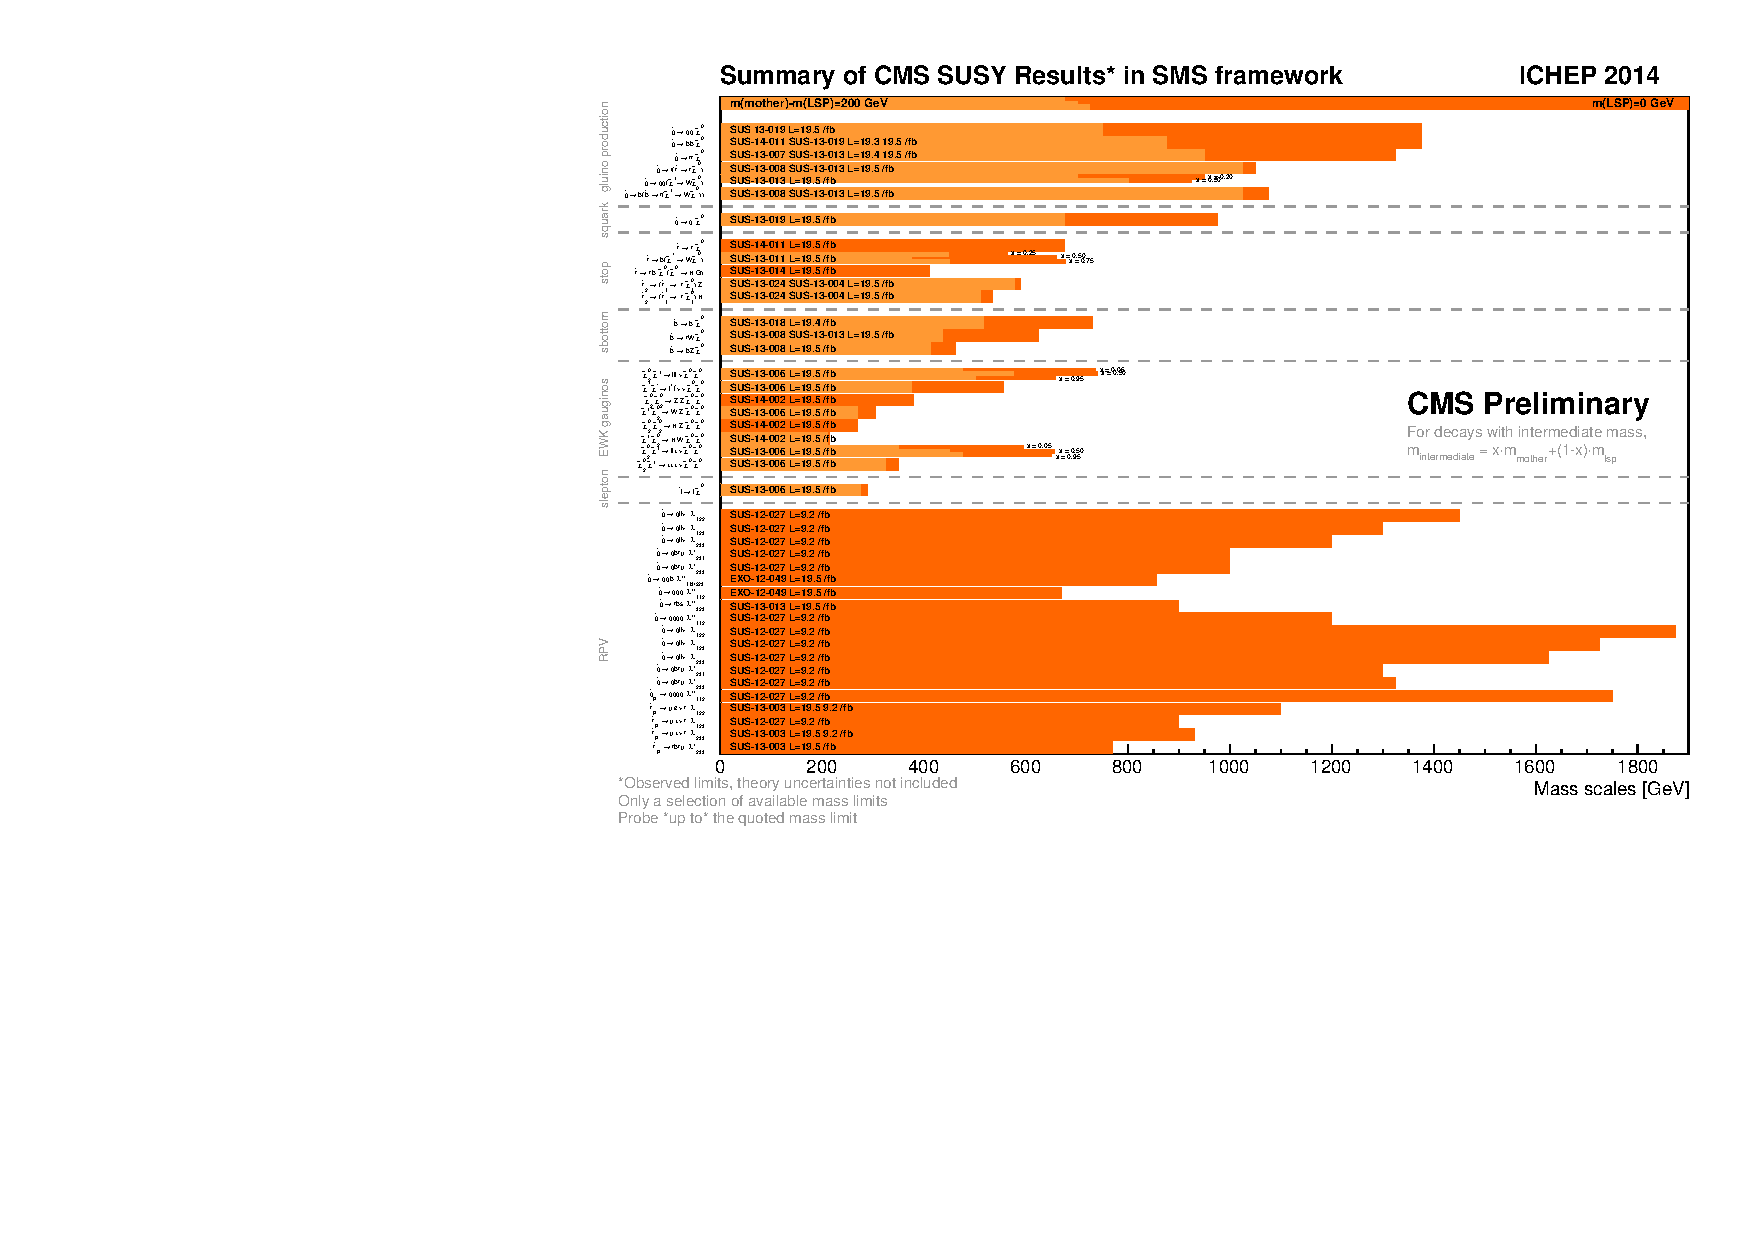
\includegraphics[height=350pt]{figures/barplot_ICHEP2014.pdf}
\caption{Summary of CMS exclusion limits for the masses of various SUSY particles with $\sqrt{s}=8\TeV$ \cite{CMS-SUSY-LIMITS}. These limits assume simplified models and unity branching fractions for the specified decays. Two scenarios are presented: the dark shades show $m(\text{LSP})=0$ and the light shades show $m(\text{mother})-m(\text{LSP})=0$.}
\label{fig:cms-susy-limits}
\end{center}
\end{figure}
\end{landscape}
}

The introduction of $R$-parity violating (RPV) terms in the SUSY Lagrangian is one way to evade these limits. If $R$-parity is violated, SUSY particles can decay to final states containing only SM particles, avoiding the characteristically large \met from the LSP, which is no longer stable. This generally eliminates the LSP as a dark matter candidate, making it a less popular option. However, RPV SUSY still solves the hierarchy problem and assists in grand unification. The possible RPV terms in the superpotential are \cite{Barbier}:
\begin{equation}
W_{\text{RPV}} = \frac{1}{2}\lambda_{ijk}\PL_{i}\PL_{j}\PE_{k}^{c} + \lambda_{ijk}^{\prime}\PL_{i}\PQ_{j}\PD_{k}^{c} + \frac{1}{2}\lambda_{ijk}^{\prime \prime}\PU_{i}^{c}\PD_{j}^{c}\PD_{k}^{c} + \mu_{i}\PL_{i}\Hone. \label{eq:WRPV}
\end{equation}
The different RPV coupling constants are denoted as $\lambda_{ijk}$, $\lambda^{\prime}_{ijk}$, $\lambda^{\prime \prime}_{ijk}$, and $\mu_{i}$, where $i$, $j$, and $k$ are generation indices. Figure \ref{fig:trilinear-RPV} shows the tree-level diagrams for the trilinear RPV couplings. As indicated by Fig. \ref{fig:trilinear-RPV} and the definition of $R$ in Eq. \eqref{eq:Rdef}, violating $R$ is equivalent to violating lepton number or baryon number. Scenarios which include all of the RPV couplings include large contributions to proton decay, due to the violation of both $B$ and $L$, and are therefore ruled out. Scenarios in which only a certain type of RPV coupling is allowed can still be viable.

\begin{figure}[hbt]
\begin{center}
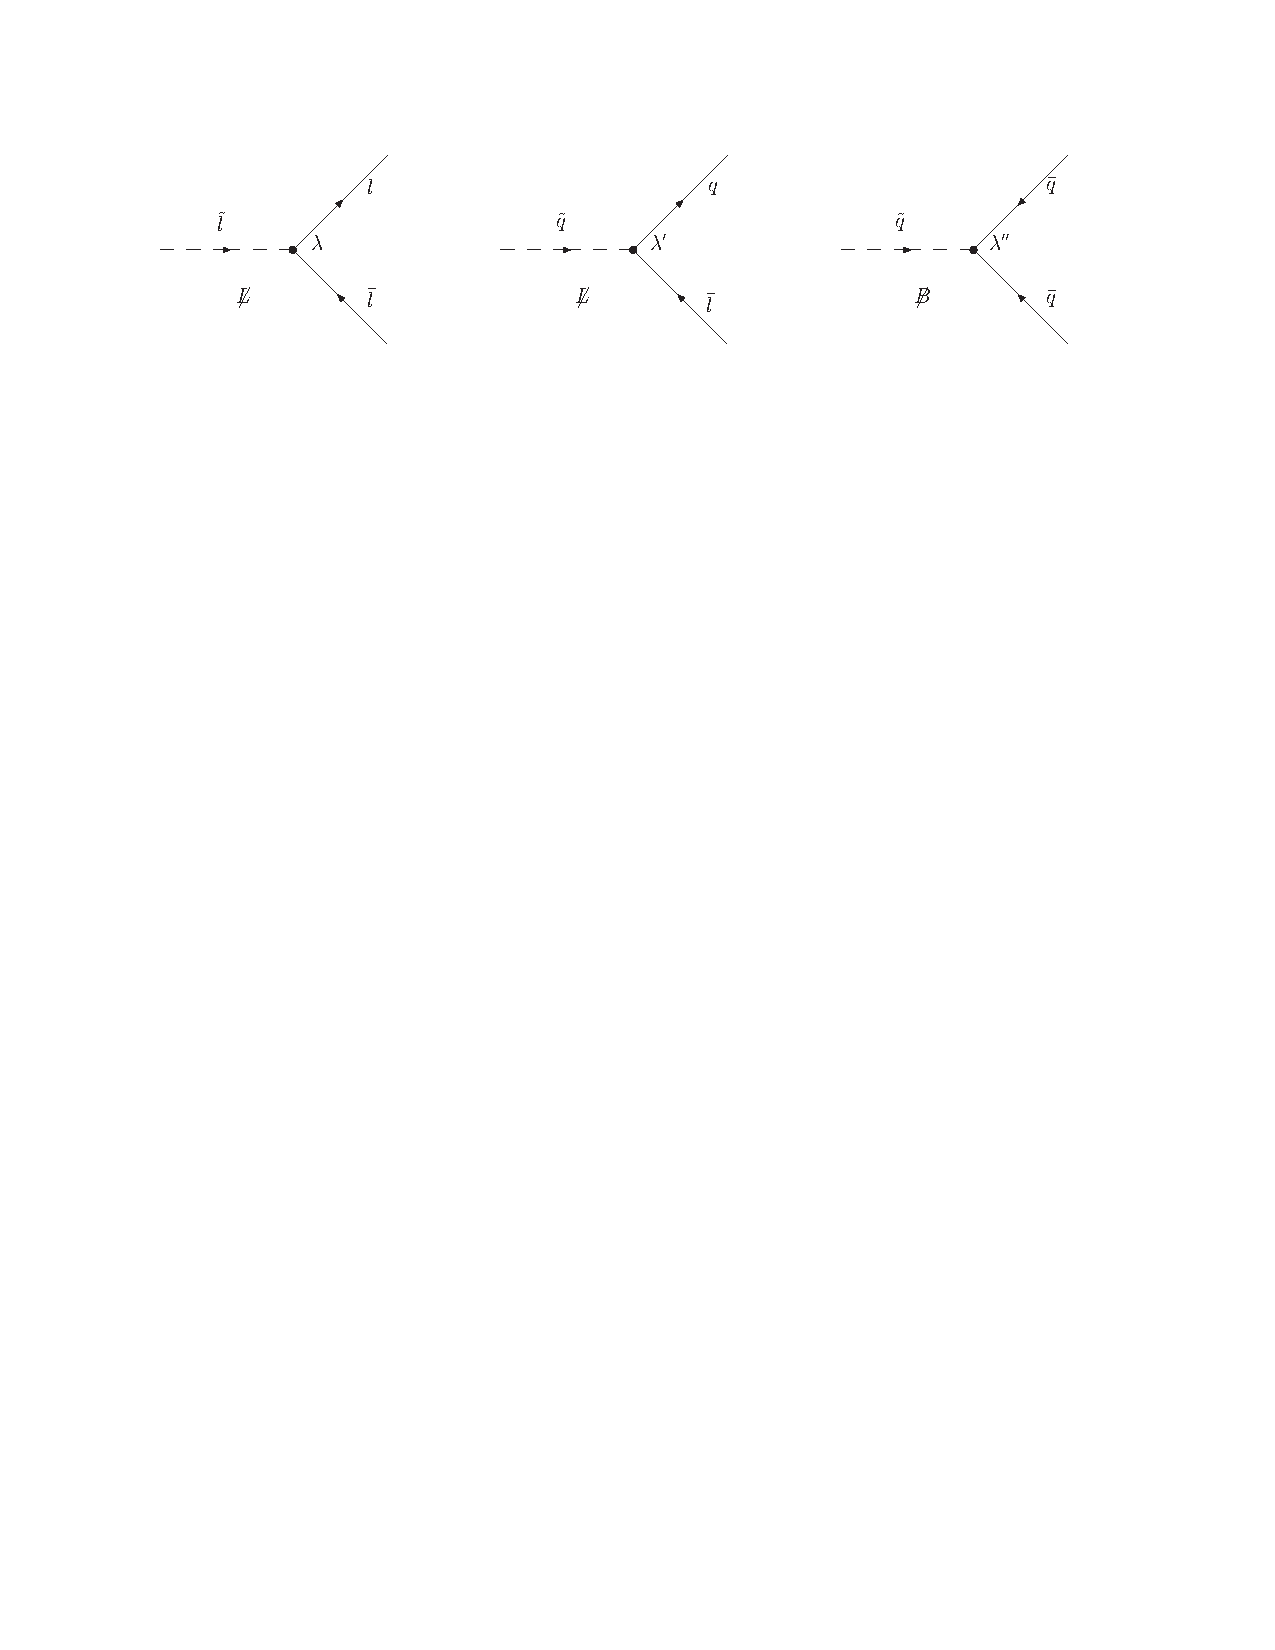
\includegraphics[width=0.95\textwidth]{figures/0406039v2_trilinear.pdf}
\caption{The LO diagrams for the three trilinear RPV couplings $\lambda$ (left), $\lambda^{\prime}$ (middle), and $\lambda^{\prime \prime}$ (right) \cite{Barbier}. These couplings violate lepton number, lepton number, and baryon number, respectively.}
\label{fig:trilinear-RPV}
\end{center}
\end{figure}

This dissertation considers the pair production of top squarks with two different RPV decays, using a decoupled model as described above. As a strongly-interacting scalar particle, the top squark production cross section is identical to the leptoquark production cross section at leading order. In decoupled models, the cross section depends on the squark mass scale and the top squark mixing angle only at higher order, and the corrections from these terms amount to less than 2\% \cite{StopCrossSec}. The first decay considered is $\sTop \rightarrow \tau \cPqb$ via the coupling $\lambda_{333}^{\prime}$. The final-state signature and kinematic distributions of this signal are identical to those from the pair production of third-generation scalar leptoquarks, as described in Sec. \ref{sec:LQ}. Therefore, the results of the leptoquark search can be directly reinterpreted to apply to the $\lambda_{333}^{\prime}$ decay of top squarks.

In some natural SUSY models, if the higgsinos are lighter than the top squark, or if the RPV couplings that allow direct decays to SM particles are sufficiently small, the top squark decay may preferentially proceed via superpartners \cite{Jared}. This motivates the second search in the dissertation, which focuses on a scenario in which the dominant RPC decay of the top squark is $\sTop \rightarrow \chipm\cPqb$. This requires the mass splitting between the top squark and the chargino to be less than the mass of the top quark, so it is chosen to be 100\GeV. The chargino is assumed to be a pure higgsino and to be nearly degenerate in mass with the neutralino, with a decay $\chipm \rightarrow \sNu\tau^{\pm} \rightarrow \cPq\cPq\tau^{\pm}$. The decay of the sneutrino occurs via the RPV coupling $\lambda_{3jk}^{\prime}$, where the cases $j, k = 1, 2$ are considered. Such a signal can only be probed by searches that do not require large \met, as chiral suppression prevents the other possible decay of the chargino, $\chipm\to\nu\sTau$, from contributing to scenarios involving the $\lambda_{3jk}^{\prime}$ coupling.

The final state from pair production of top squarks undergoing this chargino-mediated RPV decay contains two tau leptons, two b-jets, and at least four additional jets. The search for the signal with this final state is called the top squark search, to distinguish it from the similar but not identical final state in the leptoquark search. As in the leptoquark search, the analysis is divided into two channels \etau and \mutau based on the required leptonic decay of one of the tau leptons. The symbol $\mathcal{B}$ in the top squark search is used to represent the branching fraction for the decay $\sTop \rightarrow \chipm\cPqb, \chipm \rightarrow \sNu\tau^{\pm} \rightarrow \cPq\cPq\tau^{\pm}$.  This dissertation presents the first search for the chargino-mediated $\lambda_{3jk}^{\prime}$ decay of the top squark.

\renewcommand{\thesection}{\thechapter.\arabic{section}} % back to regular numbering
\chapter{Compact Muon Solenoid Experiment
\label{ch:cmsexperiment}}
%\setcounter{section}{-1}

The Compact Muon Solenoid (CMS) experiment is one of two general-purpose detectors at the LHC. It is located about 100\unit{m} underground on the LHC ring, near Cessy, France. The detector is cylindrically shaped, with a total length of 22\unit{m}, a diameter of 15\unit{m}, and a weight of 14000\unit{tons}. Figure \ref{fig:cms-overall} shows the overall layout of the detector. The following sections describe the LHC (based on Ref. \cite{LHCmachine}) and the CMS subdetector systems (based on Ref. \cite{CMSJINST}).

\begin{figure}[hbt]
\begin{center}
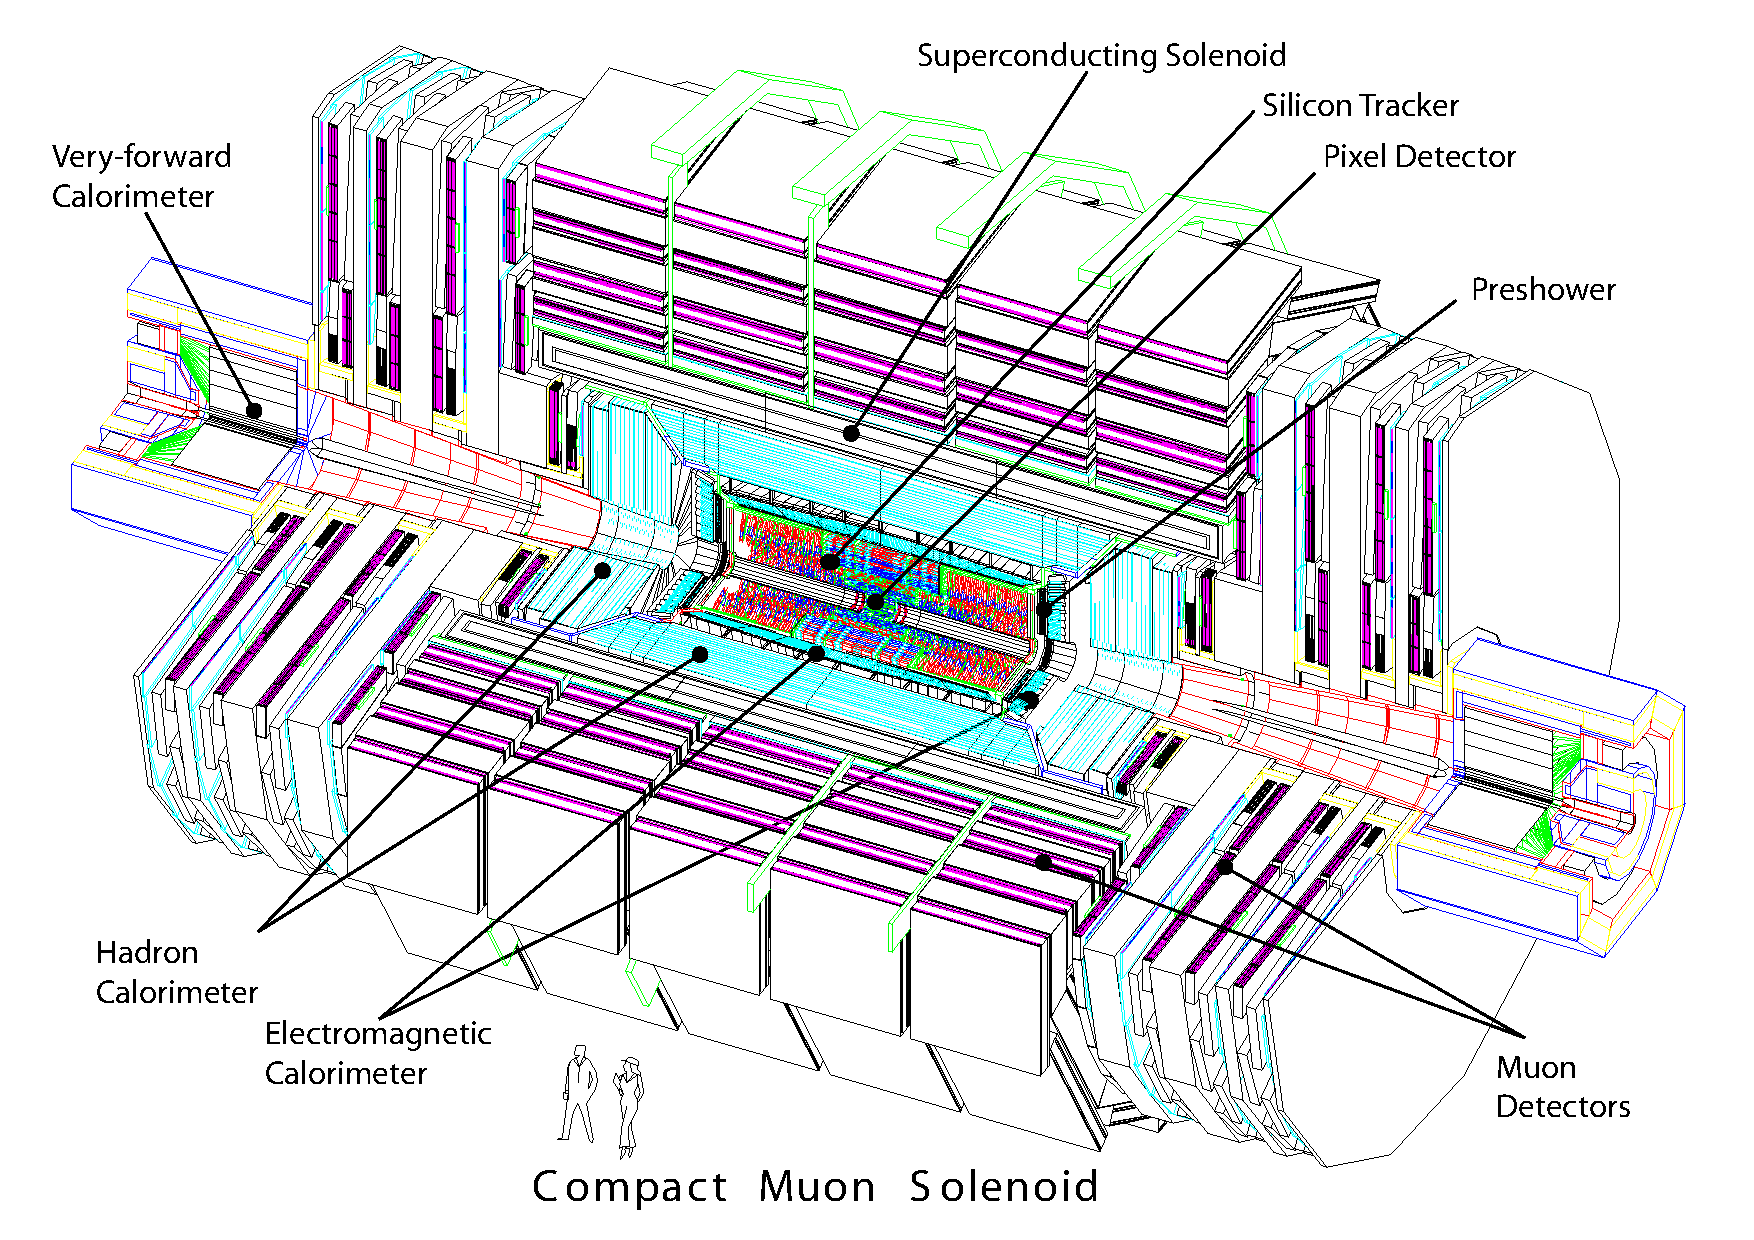
\includegraphics[width=0.95\textwidth]{figures/cms_complete_labelled.pdf}
\caption{The layout of the CMS detector, with the subdetectors labeled and two humans shown for a height reference.}
\label{fig:cms-overall}
\end{center}
\end{figure}

The center of the detector, the interaction point (IP), is used as the origin of the right-handed coordinate system that describes locations and directions within the detector. The $z$-axis is assigned to the direction of the LHC beam line. The polar angle $\theta$ is often transformed into pseudorapidity, defined as $\eta = -\text{ln}[\text{tan}(\theta/2)]$. Differences in pseudorapidity are Lorentz invariant for boosts in the $z$ direction, and particle production is approximately uniform in $\eta$. The plane transverse to the $z$-axis comprises the $x$- and $y$-axes, with the $x$-axis pointing toward the center of the LHC ring and the $y$-axis pointing upward in the normal direction. The azimuthal angle $\phi$ and the radial coordinate $r$ are also defined in the transverse plane. The magnitude of the component of momentum in the transverse plane is labeled \pt.

\section{The Large Hadron Collider}

The Large Hadron Collider is the largest machine ever built and the highest-energy collider in the world. It uses the tunnel originally constructed for the Large Electron-Positron Collider (LEP), with a circumference of 26.7\unit{km}. The tunnel is located underground in Switzerland and France, near Geneva. Figure \ref{fig:lhc-diagram} shows a diagram of the LHC. The location of the CMS experiment is provided and the other major experiments are also indicated.

\begin{figure}[hbt]
\begin{center}
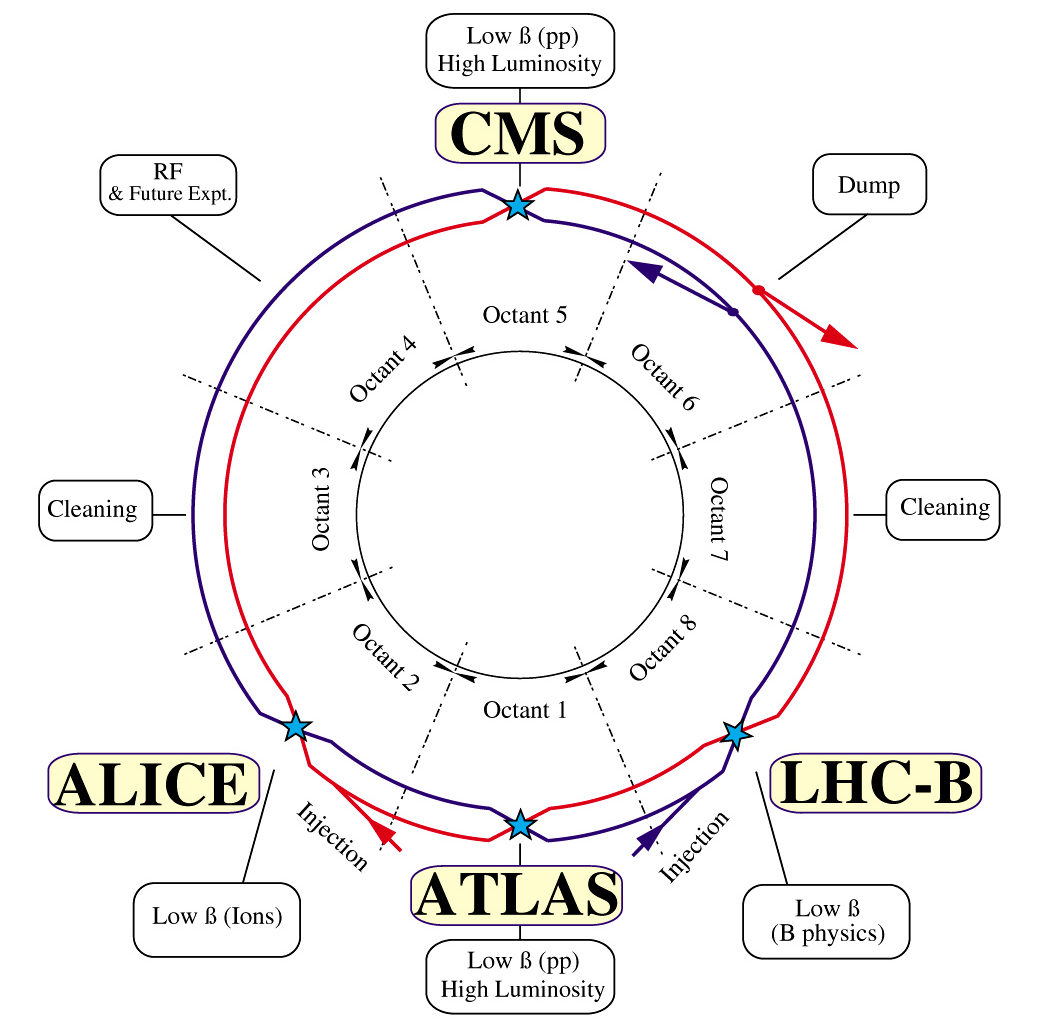
\includegraphics[width=0.95\textwidth]{figures/lhc-pho-1997-060.png}
\caption{A diagram of the LHC with the major experiments labeled \cite{Jean-Luc:841573}.}
\label{fig:lhc-diagram}
\end{center}
\end{figure}

The LHC is designed to accelerate two beams of protons up to energies of 7\TeV each, at instantaneous luminosities up to $10^{34}\percms$. The use of supercooled superconducting magnets, discussed below, is crucial. Several stages of CERN accelerators are used to inject proton beams into the LHC, as shown in Fig. \ref{fig:lhc-injectors}. These include the linear accelerator Linac2, the Proton Synchrotron Booster (PSB), the Proton Synchrotron (PS), and the Super Proton Synchrotron (SPS). The accelerated protons are grouped into bunches using radio frequency (RF) electromagnetic fields. The LHC is designed to accommodate a bunch spacing of 25\unit{ns}, with $10^{11}$ protons per bunch and 2808 bunches per beam.

\begin{figure}[hbt]
\begin{center}
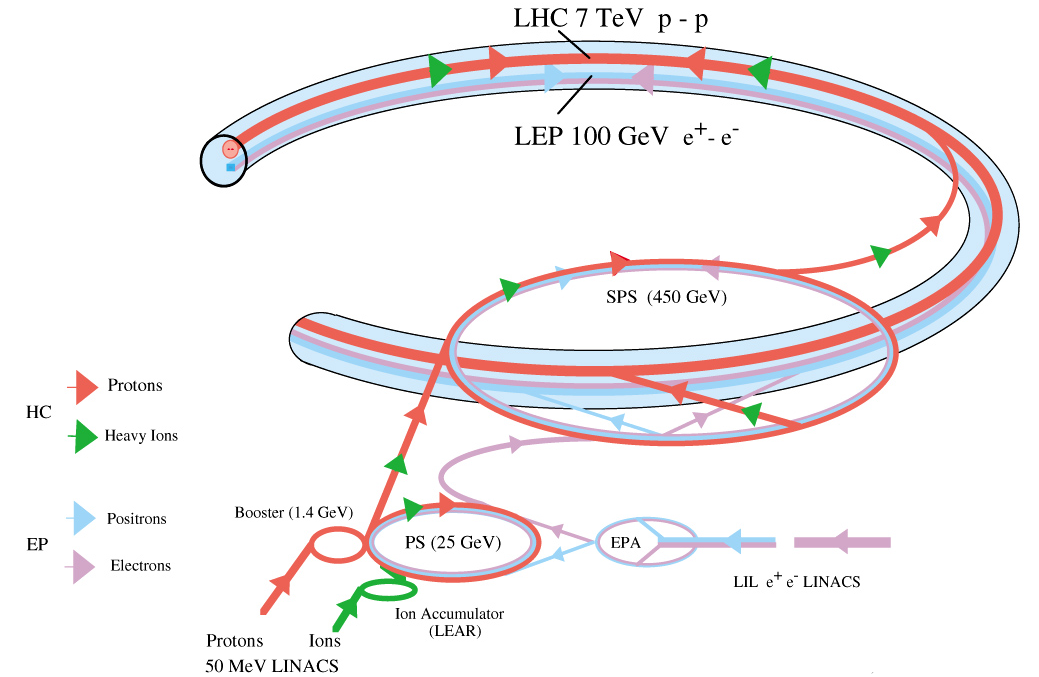
\includegraphics[width=0.95\textwidth]{figures/lhc-pho-1993-008.png}
\caption{A diagram of the CERN accelerators which form the LHC injector \cite{Jean-Luc:841568}.}
\label{fig:lhc-injectors}
\end{center}
\end{figure}

Due to size limitations in the tunnel, the two rings used to accelerate the two proton beams are formed by twin bore magnets. Each magnet has a single mechanical structure and cryostat, in which are placed two coils and two beam channels. The dipole magnet coils use superconducting NbTi Rutherford cables cooled to 1.9\unit{K}, as shown in Fig. \ref{fig:lhc-dipole}, with a design field strength of 8.33\unit{T} for acceleration of protons up to 7\TeV. This extreme cooling is accomplished using superfluid helium. In total, the LHC contains 1232 dipole magnets. Thousands of quadrupole, sextupole, octupole, and decapole magnets are used to correct and focus the beam.

\begin{figure}[hbt]
\begin{center}
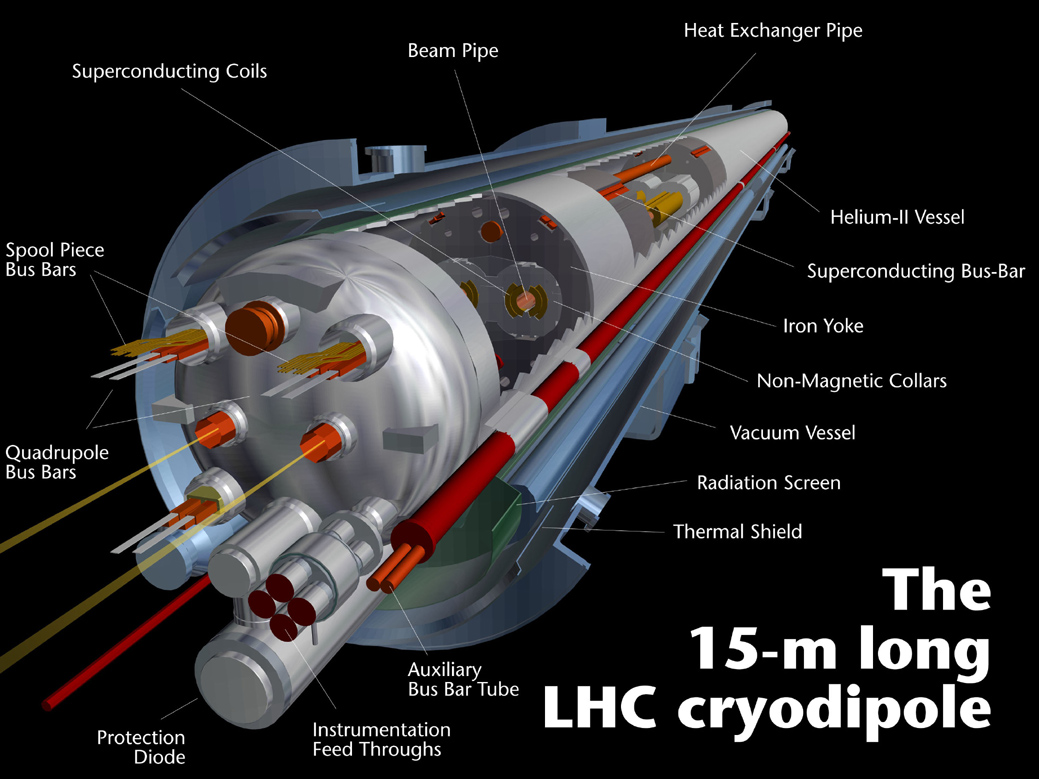
\includegraphics[width=0.95\textwidth]{figures/lhc-pho-1998-299.jpg}
\caption{A diagram of an LHC dipole magnet, with the major components labeled \cite{Dailler:842253}.}
\label{fig:lhc-dipole}
\end{center}
\end{figure}

In 2012, the LHC accelerated proton beams to energies of 4\TeV each, with a peak instantaneous luminosity of $7.67\times10^{33}\percms$ and a bunch spacing of 50\unit{ns}. During that year, it delivered 23.30\fbinv of integrated luminosity to the CMS detector, of which 21.79\fbinv was recorded \cite{LumiPublic}. In the upcoming 2015 run, the LHC will achieve its design energy, instantaneous luminosity, and bunch spacing.

\section{Tracker}
\label{sec:tracker}

The CMS tracker is the first subdetector to measure charged particles produced in collisions at the IP. It is 5.8\unit{m} long and 2.5\unit{m} in diameter, covering the pseudorapidity range $-2.5 < \eta < 2.5$. Two subsystems make up the tracker: the pixel detector and the silicon strip tracker. The layout of the tracker, with these subsystems labeled, is shown in Fig. \ref{fig:tk-layout}. Due to the tracker's location close to the IP, it experiences severe radiation doses that are expected to range from 0.18 to 84\unit{Mrad} after 500\fbinv of data. Hence, the tracker must be robust against radiation damage, requiring operation at $-10\degC$ and influencing the design of the sensors and electronics. For tracks with momentum of 100\GeV, the tracker has a transverse momentum resolution of 1--2\% for $|\eta|<1.6$; at higher $\eta$, the reduced transverse depth of the tracker degrades the resolution.

\begin{figure}[hbt]
\begin{center}
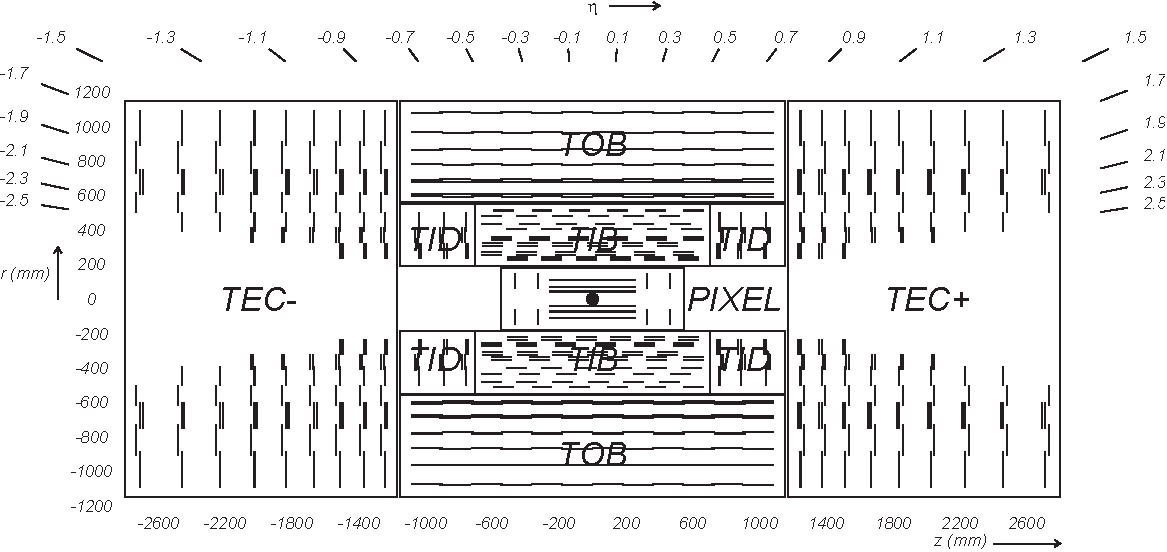
\includegraphics[width=0.95\textwidth]{figures/CMS_tracker.pdf}
\caption{The layout of the CMS tracker, with subsystems labeled.}
\label{fig:tk-layout}
\end{center}
\end{figure}

The pixel detector is the innermost portion of the tracker. It consists of three barrel layers, collectively called BPIX, and two endcap layers, called FPIX. Each pixel cell is a hybrid silicon detector with dimensions $100\times150\mum^{2}$. The small pixel size enables precise track resolutions of 10\mum in the $r$-$\phi$ direction and 20\mum in the $z$ direction. In total, the BPIX comprises 48 million pixels and the FPIX comprises 18 million pixels. The pixel detector is important for many key components of CMS physics analysis. These include the reconstruction of secondary vertices from decays of tau leptons and bottom quarks, as well as producing seed tracks for the strip tracker and the high level trigger.

The silicon strip detector consists of four subsystems. The Tracker Inner Barrel (TIB) has four layers with the three-layer Tracker Inner Disks (TID) at each end; both systems' strips are 320\mum thick. Surrounding the TIB/TID is the Tracker Outer Barrel (TOB), which has six layers. The first four layers of the TOB use 500\mum thick strips, while the last two layers use 122\mum thick strips. The Tracker EndCaps (TEC) have nine disks with up to seven layers of strips, 320\mum thick in the inner four rings and 500\mum thick in the outer three rings. In total, all of these layers contain 9.3 million silicon strips.

The tracker maintained excellent performance during the 2012 run of the LHC. The pixel detector had 97.7\% of channels operational in BPIX and 92.8\% of channels operational in FPIX, while 97.5\% of channels in the strip detector were active. The hit reconstruction efficiencies were greater than 99\% for each layer of the strip detector and greater than 99.5\% for each layer of the pixel except for the first layer of BPIX, which had an efficiency greater than 99.2\% \cite{Veszpremi:2014hpa}. 

\section{Electromagnetic Calorimeter}

The electromagnetic calorimeter (ECAL) is a homogeneous calorimeter constructed entirely of lead tungstate (\pbwo) crystals. The ECAL is divided into two subsystems: the ECAL barrel (EB) and the ECAL endcap (EE). In the endcap region, there is an additional ECAL preshower (ES) detector in front of the EE. Figure \ref{fig:ecal-layout} displays these subsystems. \pbwo has a peak emission wavelength of 425\unit{nm} and many desirable material properties. These properties include high density ($8.28\unit{g/cm}^3$), short radiation length (0.89\cm), short Moli\`{e}re radius (2.2\cm), and fast decay time (6\unit{ns}). The use of homogeneous \pbwo crystals enables precise energy resolution for electromagnetic objects. For photons with $\ET \approx 60\GeV$, the energy resolution ranges from 1.1\% to 2.6\% for the EB and 2.2\% to 5.0\% for the EE. In general, the energy resolution $\sigma$ varies as a function of energy $E$ in \GeVns:
\begin{equation}
\label{eq:ecal-res} \left(\frac{\sigma}{E}\right)^{2} = \left(\frac{S}{\sqrt{E}}\right)^{2} + \left(\frac{N}{E}\right)^{2} + C^{2}.
\end{equation}
In Eq. \eqref{eq:ecal-res}, $S$ is the stochastic term, $N$ is the noise term, and $C$ is the constant term. Typical values for these terms were measured by a test beam to be $S=2.8\%$, $N=12\%$, $C=0.30\%$.

\begin{figure}[hbt]
\begin{center}
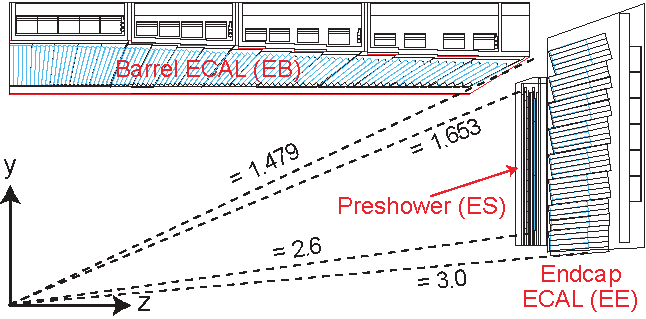
\includegraphics[width=0.95\textwidth]{figures/ECAL_transverse_section.pdf}
\caption{A diagram of the CMS ECAL, with subsystems and $\eta$ ranges labeled.}
\label{fig:ecal-layout}
\end{center}
\end{figure}

The EB contains 61200 \pbwo crystals and covers the range $|\eta|<1.479$. The crystals are arranged in a projective geometry with a tapered shape. The crystal granularity is approximately $0.0174\times0.0174$ in $\eta$-$\phi$, corresponding to dimensions of $22\times22\mm^{2}$ at the front face and $26\times26\mm^{2}$ at the back face. The EB has a depth of 230\mm or 25.8 radiation lengths ($X_{0}$). The scintillation light produced by the \pbwo crystals is read out using avalanche photodiodes (APDs). At 18\degC, the APDs measure approximately 4.5 photoelectrons per \MeVns. The dark current of the APDs is sensitive to radiation exposure. Over the course of the 2012 run, the dark current ranged from 0.3--1.3\muA on average, corresponding to an average noise of 47--57\MeV \cite{CMS:2013ecal}.

The EE contains 14648 \pbwo crystals and covers the range $1.479<|\eta|<3.0$. The crystals are arranged in a non-projective $x$-$y$ geometry, with dimensions of $28.62\times28.62\mm^{2}$ at the front face and $30\times30\mm^{2}$ at the back face. The EE has a depth of 220\mm or 24.7$\,X_{0}$. Vacuum phototriodes (VPTs) are used as the photodetectors to read out the scintillation light from the \pbwo crystals. They collect approximately 4.5 photoelectrons per \MeVns at 18\degC. During the 2012 run, the average noise ranged from 180--220\MeV, with a more dramatic increase up to 600\MeV at high $\eta$ because of the high radiation dose \cite{CMS:2013ecal}.

The ES is intended to identify neutral pions in the endcap region, covering the range $1.653<|\eta|<2.6$. It is a sampling calorimeter with two layers of lead absorber and silicon strip detectors. The first layer of lead absorber has a thickness of 2$\,X_{0}$, while the second layer has a thickness of 1$\,X_{0}$. Each layer of silicon strips is 320\mum thick and can collect 3.6\unit{fC} of charge from a minimum ionizing particle.

%add percentage of live channels for EB and EE in 2012 run? and HE raddam?

\section{Hadron Calorimeter}

The hadron calorimeter (HCAL) is a sampling calorimeter which measures the energy of hadrons. The HCAL is especially important for measuring neutral hadrons, which do not leave tracks in the tracker. In addition, by containing all hadronic activity in each event within $|n|<5$, the HCAL enables the measurement of \met caused by neutrinos and other theoretical weakly-interacting particles. The HCAL consists of four subsystems. Three of these subsystems use similar technology: the HCAL barrel (HB), the HCAL endcap (HE), and the HCAL outer (HO). The fourth subsystem, the HCAL forward (HF), uses an alternative technology necessary to survive the high radiation doses at its forward location. The locations of the various HCAL subsystems in the CMS detector are shown in Fig. \ref{fig:hcal-layout}. The calorimeter system, combining the ECAL and the HCAL, can measure jets with a resolution $\sigma/E \approx 100\% / \sqrt{E\,[\GeVns]} \oplus 5\%$ that varies with the jet energy $E$.

\begin{figure}[hbt]
\begin{center}
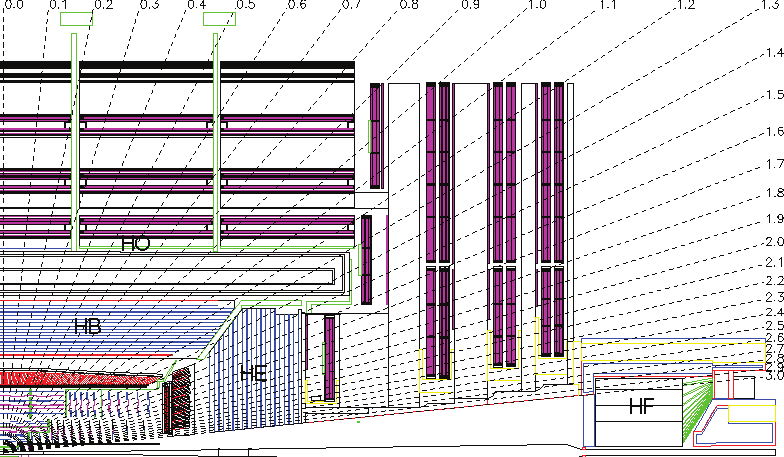
\includegraphics[width=0.95\textwidth]{figures/HCAL_subdet.pdf}
\caption{The layout of the HCAL subsystems HB, HE, HO, and HF in the CMS detector.}
\label{fig:hcal-layout}
\end{center}
\end{figure}

The HB is a 16-layer sampling calorimeter covering the range $|\eta|<1.3$. The absorbing layers are made of C26000 cartridge brass, composed of 70\% copper and 30\% zinc. Cartridge brass has a density of $8.53\unit{g/cm}^3$, a radiation length of 1.49\cm, and a nuclear interaction length of 16.42\cm. The first absorbing layer in the HB is a 40-mm-thick steel plate. The next eight absorbing layers are 50.5-mm-thick brass plates, and the subsequent six absorbing layers are 56.5-mm-thick brass plates. The last absorbing layer is a 75-mm-thick steel plate. The overall thickness of the HB absorber ranges from 5.82 nuclear interaction lengths ($\lambda_{0}$) at $\eta=0$ to 10.6$\,\lambda_{0}$ at $|\eta|=1.3$. The EB in front of the HB has a thickness of 1.1$\,\lambda_{0}$ and can measure the electromagnetic portions of early developing hadronic showers. The scintillating layers consist of 3.7-mm-thick Kuraray SCSN81 plastic scintillator, a polystyrene base doped with fluors. The exception is Layer 16, which has a thickness of 9\mm, in order to sample more from late developing hadronic showers. At the front of the HB, before the first absorbing layer, is the scintillator Layer 0, which is 9\mm of Bicron BC408 plastic scintillator, a polyvinyltoluene base doped with fluors. Layer 0 samples the energy deposited by hadronic showers in the dead material between the EB and the HB. The scintillator tiles are arranged in a projective geometry with a granularity of $0.087\times0.087$ in $\eta$-$\phi$. In total, the HB has 16 $\eta$ divisions, 36 $\phi$ divisions, and approximately 70000 tiles. The light from the scintillators is collected by Kuraray Y-11 green wavelength shifting (WLS) fiber, which is placed in a groove shaped like the Greek letter $\sigma$ in the scintillator tiles. The wavelength-shifted light from multiple layers is brought together and read out by hybrid photodiodes (HPDs). These photodetectors were chosen because of their large dynamical range and low sensitivity to magnetic fields.

The thinness of the HB at low $\eta$ prevents it from fully containing hadronic showers, so the HO is added to act as an extension of the calorimeter system. The HO uses the same scintillator tile technology as the HB: 3.7-mm-thick SCSN81 with Y-11 WLS fiber and granularity $0.087\times0.087$ in $\eta$-$\phi$, read out by HPDs. The HO is divided into five rings, each with a width of 2.536\unit{m} in the $z$ direction, based on the structure of the iron return yoke outside of the solenoid. In the central Ring 0, the HO has two scintillating layers, one inside the solenoid and one outside of it. In the other rings, the HO has one scintillating layer outside of the solenoid. The thickness of the absorbing iron layer formed by the solenoid is 19.5\cm, extending the total depth of the calorimeter system to a minimum of 11.8$\,\lambda_{0}$.

The HE is a 17-layer sampling calorimeter covering the range $1.3<|\eta|<3.0$. Each absorbing layer consists of 79-mm-thick cartridge brass, the same material used for the HB absorbing layers. The scintillating layers use the same technology as the HB and the HO. In total, the HE contains 20916 scintillator tiles. The granularity of the tiles is the same as HB for $|\eta|<1.6$; for higher $\eta$, they become coarser, with a granularity of approximately $0.17\times0.17$ in $\eta$-$\phi$. Unlike the HB, the scintillating layers in each tower are split into multiple groups called depths before being read out by HPDs. A diagram of the depth segmentation scheme is shown in Fig. \ref{fig:hcal-depths}. This depth segmentation allows for more precise recalibration of the HE, which experiences a higher radiation dose than the HB. Towers 27, 28, and 29, which are the closest to the beamline, have three readout depths, while the other towers have two readout depths. The crossover region between the HB and the HE, towers 15 and 16, also utilize depth segmentation. As in the HB, Layer 0 in the HE consists of 9-mm-thick BC408 to sample from the dead material between the EE and the HE. The combined calorimeter system, including both the EE and the HE, has an approximate thickness of 10$\,\lambda_{0}$.

The HF covers the range $3.0<|\eta|<5.0$, with no ECAL in front of it. It consists of a steel absorber structure with a thickness of 165\cm or 10$\,\lambda_{0}$. Polymer-cladded quartz fibers with diameter 800\mum are embedded in the steel absorber. The fibers are bundled together to form 13 towers in a non-projective $x$-$y$ geometry with granularity $0.175\times0.175$ in $\eta$-$\phi$. Over 1000\unit{km} of fiber is used in the HF. Half of the fibers run for the full 165\cm depth of the detector, while the other half start 22\cm into the detector. Electromagnetic showers deposit most of their energy in the first 22\cm of the HF, while hadronic showers deposit energy throughout the HF. Therefore, by reading out each type of fiber separately, the two types of showers can be distinguished. The fibers measure particle showers using Cherenkov light, which is read out by photomultiplier tubes (PMTs). They measure approximately 1 photoelectron for every 4\GeV of energy deposited. This alternative design was necessary to ensure the radiation hardness of the HF, parts of which can experience 100\unit{Mrad/year}.

\begin{figure}[hbt]
\begin{center}
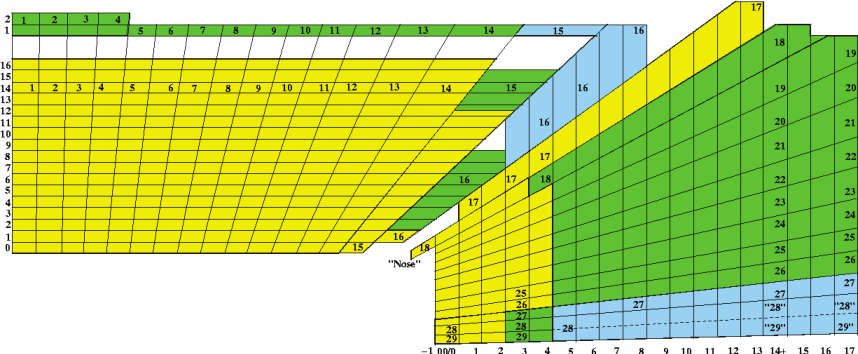
\includegraphics[width=0.95\textwidth]{figures/HCAL_tower_segmentation.pdf}
\caption{A diagram of the depth segmentation scheme in the HB and the HE.}
\label{fig:hcal-depths}
\end{center}
\end{figure}

%add percentage of live channels for HCAL in 2012 run?

\section{Solenoid}

The superconducting solenoid is the central feature of the CMS detector. The solenoid provides a magnetic field of 3.8\unit{T} within the volume formed by its diameter of 6\unit{m} and length of 12.5\unit{m}. This strong magnet field is necessary so that high energy charged particles bend sufficiently for the tracker to measure their momenta accurately. At full current, the solenoid has a stored energy of 2.35\unit{GJ}. The magnet is constructed from a 4-layer winding of reinforced NbTi conductor, cooled to 4.5\unit{K}. It is split into five rings of equal length. The cold mass of the magnet is 220 tons, and the high ratio between the stored energy and the cold mass, 11.6\unit{KJ/kg}, causes a significant mechanical deformation of 0.15\% when the magnet is powered. Figure \ref{fig:solenoid} shows an artistic rendering of the solenoid.

\begin{figure}[hbt]
\begin{center}
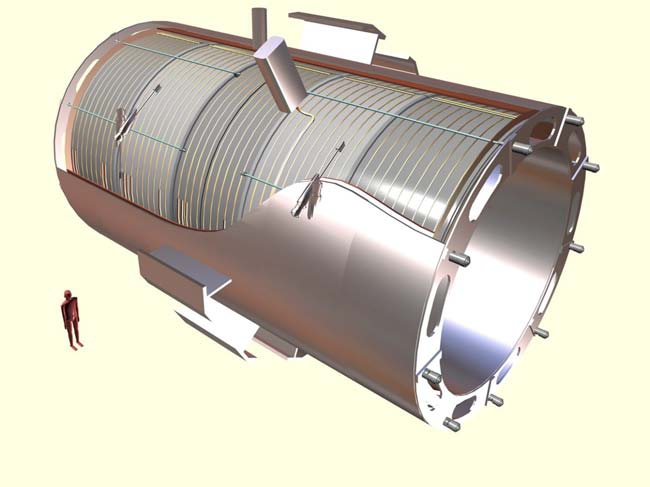
\includegraphics[width=0.95\textwidth]{figures/CMS_solenoid.jpg}
\caption{An artistic rendering of the CMS solenoid, showing the five rings placed inside the cryostat, along with the support structure.}
\label{fig:solenoid}
\end{center}
\end{figure}

\section{Muon System}
\label{sec:muon-system}

The identification and measurement of muons is a major focus of the CMS experiment. The CMS muon system comprises three subsystems, each utilizing different gaseous particle detection technologies. In the barrel region, drift tubes (DTs) are used. In the endcap region, cathode strip chambers (CSCs) are used. Resistive plate chambers (RPCs) are also used in both regions. The muon systems are built into the iron yoke, which consists of five barrel rings and six endcap disks weighing 10000 tons in total. The yoke confines the outer magnetic field from the return flux from the solenoid and absorbs stray hadrons. The layout of the muon system is shown in Fig. \ref{fig:muon-system}. The momentum resolution of the muon system by itself is approximately 9\% for $\pt<200\GeV$ with low $\eta$ and low $p$. For 1\TeV muons, the resolution varies between 15\% and 40\%, depending on $|\eta|$. When the muon system measurements are combined with measurements from the tracker, the 1\TeV muon resolution is improved to 5\%.

\begin{figure}[hbt]
\begin{center}
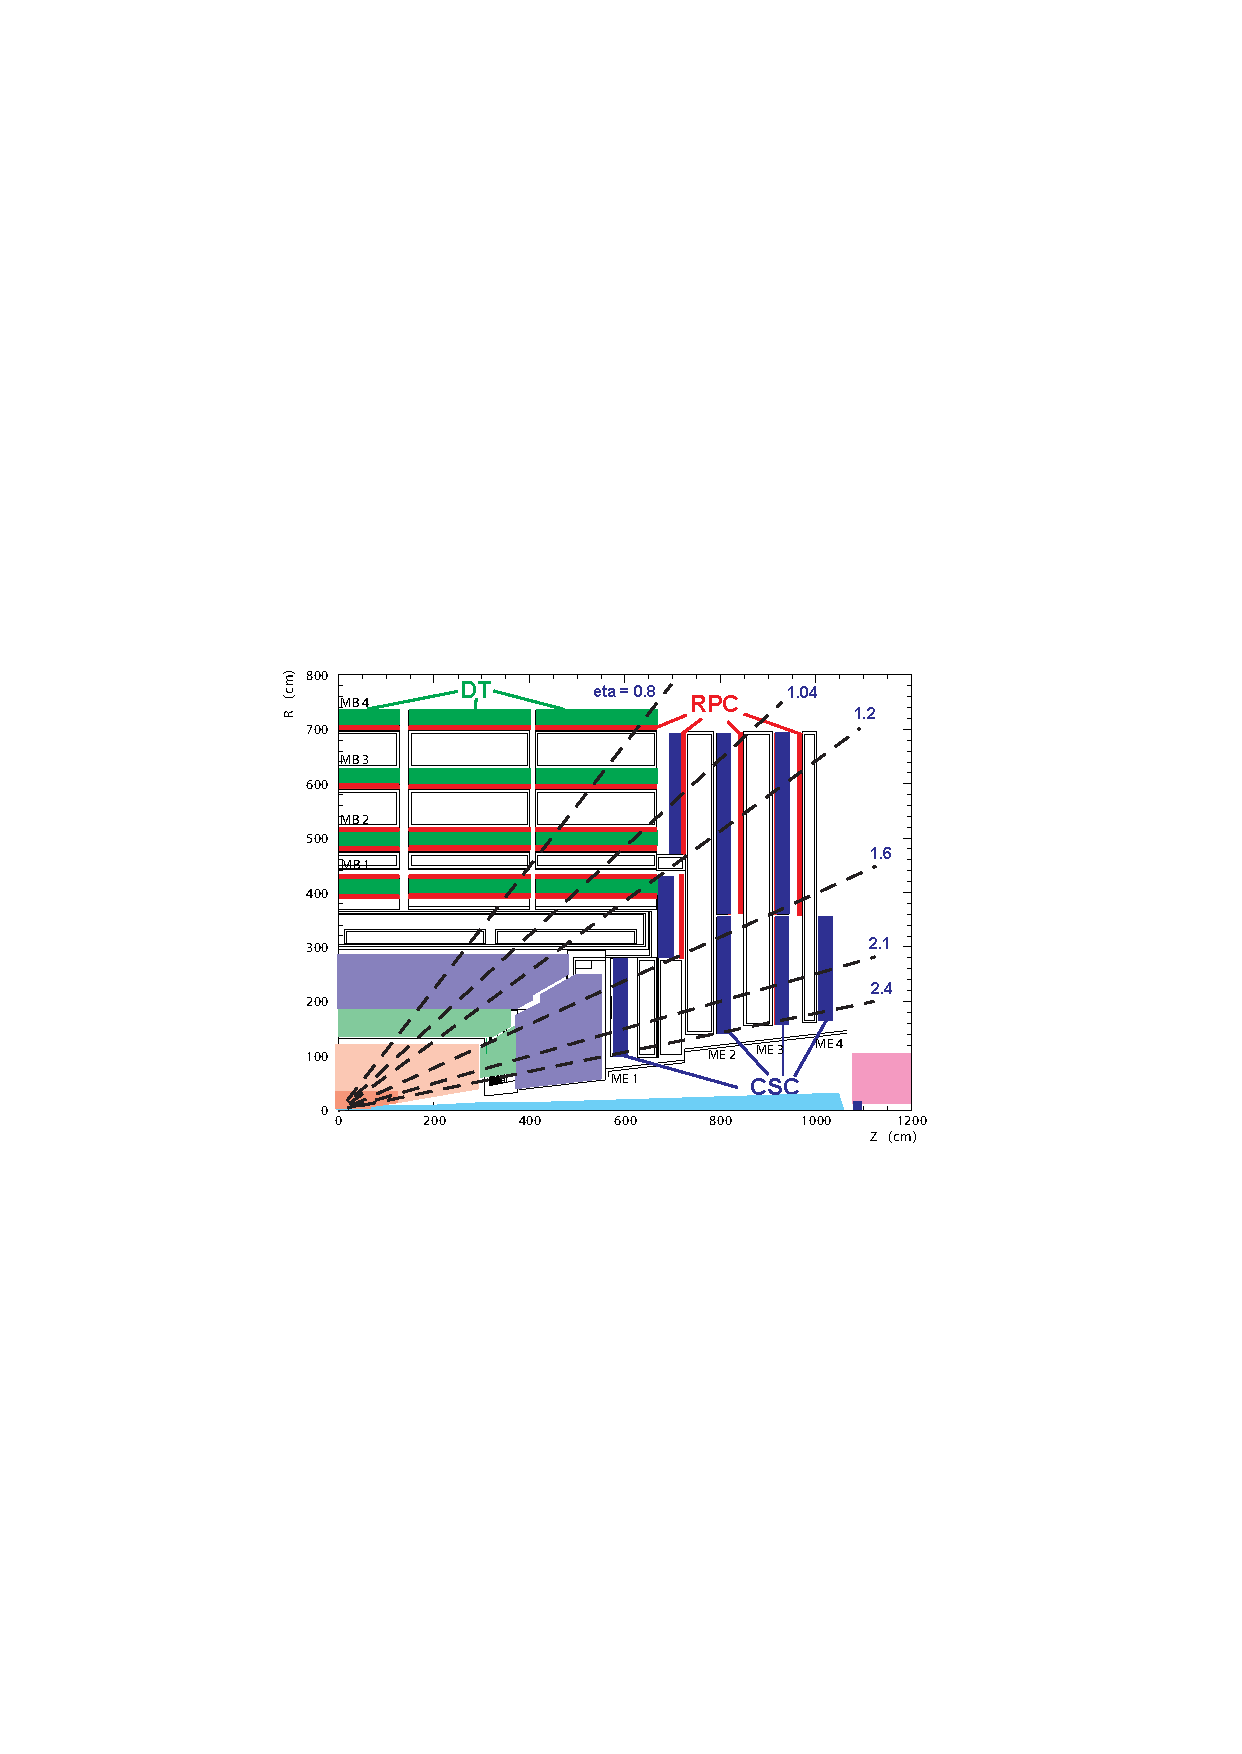
\includegraphics[width=0.95\textwidth]{figures/CMS_muon_system.pdf}
\caption{The layout of the muon system, with the three subsystems labeled.}
\label{fig:muon-system}
\end{center}
\end{figure}

The DTs are divided into four stations, which together cover the range $|\eta|<1.2$ and are labeled MB1 through MB4 (Muon Barrel). The first three stations each contain twelve chambers divided into three groups of four. Two of the groups of four measure the $r$-$\phi$ coordinate of muons, while the third group of four measures the $z$ coordinate. MB4 does not include a group of chambers that measures $z$. All four stations together contain 250 DTs with a total of 172000 sensitive wires. The gas used in the DTs is a mixture of 85\% Ar and 15\% $\text{CO}_2$, and the anode wires are gold-plated stainless steel with a diameter of 50\mum. Within $|\eta|<0.8$, the MB stations alone can reconstruct high-\pt muon tracks with an efficiency exceeding 95\%. The global $r$-$\phi$ resolution is 100\mum.

The CSCs are also divided into four stations and cover the range $0.9<|\eta|<2.4$. The four stations are labeled ME1 through ME4 (Muon Endcap). Each station is divided into several groups as follows: ME1 has three groups of 72 CSCs; ME2 and ME3 each have one group of 36 CSCs and another group of 72 CSCs; ME4 has one group of 36 CSCs. The total number of CSCs is thus 468. The cathode strips are arranged in the radial direction to measure the $r$-$\phi$ coordinate, while the anode wires are perpendicular to the strips to measure $\eta$. There are approximately 220000 cathode strip readout channels and 180000 anode wire readout channels. The CSC gas mixture is set at 40\% AR, 50\% $\text{CO}_2$, and 10\% $\text{CF}_4$. The cathode strips are formed from a fiberglass/epoxy material called FR4, coated with 36-$\mu$m-thick copper. The anode wires are made of gold-plated tungsten with a diameter of 50\mum. The first group of ME1 CSCs uses slightly thinner wire with 30\mum diameter and has some other slightly modified properties.

To complement the DTs and CSCs, RPCs are installed in both the barrel and endcap regions, covering the range $|\eta|<1.6$. The RPCs are primarily used to provide muon trigger information, due to fast tagging capabilities which allow them to precisely identify the bunch crossing time of muon candidate events. The time resolution of the RPCs is less than 3\unit{ns}, compared to maximum drift times of 400\unit{ns} for the DTs and 60\unit{ns} for the CSCs. MB1 and MB2 each have one internal and one external group of RPCs, relative to the DTs; MB3 and MB4 each have two internal groups of RPCs. These groups together comprise 480 chambers. In the endcap, there are three RPC stations mounted in concentric circles on the iron yoke disks, with a total of 144 chambers. The RPCs are parallel plate detectors filled with a gas mixture of 96.2\% $\text{C}_2\text{H}_2\text{F}_4$, 3.5\% $i\text{C}_4\text{H}_{10}$, and 0.3\% $\text{SF}_6$.

%add percentage of live channels for muon system in 2012 run?

\section{Trigger}

The LHC operates at a high instantaneous luminosity, up to $10^{34}\percms$. With an expected proton-proton cross section of 100\unit{mb} at the LHC center-of-mass energies, the collision rate is approximately 1\unit{MHz}. The CMS trigger is necessary to reduce this high rate of collision events to a rate which can be stored and processed. The trigger system consists of two stages. The first stage uses hardware and is called the Level-1 (L1) Trigger. The L1 Trigger is designed to have a maximum output rate of 100\unit{kHz}. The second stage is the High Level Trigger (HLT), which uses software and reduces the output rate to $\mathcal{O}(100\unit{Hz})$.

The L1 Trigger uses custom-built programmable electronics, including field-programmable gate arrays (FPGAs), memory lookup tables (LUTs), and application-specific integrated circuits (ASICs). All of the subdetectors send input to the L1 Trigger, which is organized into local, regional, and global components as shown in Fig. \ref{fig:L1-trigger}. The local components, Trigger Primitive Generators (TPGs), are constructed from energy deposits in the calorimeters and track segments or hit patterns from the muon system.

The TPGs from the ECAL, the HCAL, and the HF are combined into the Regional Calorimeter Trigger (RCT). The RCT groups calorimeter trigger towers into regions, which are made up of four towers in the barrel and endcap, and one tower in the HF. These regions are used to determine electron and photon candidates, as well as transverse energy sums (\sumet) and tau-jet vetoes. The RCT also passes information to the muon triggers about minimum ionizing particle (MIP) energy deposits and surrounding energy deposits that indicate whether muon candidates are isolated from other particles. Using information from the RCT, the Global Calorimeter Trigger (GCT) determines jet candidates and counts, providing up to four jets and four tau-jets from the central HCAL and four jets from the HF. The GCT also determines total \ET, \met, and \HT, which is calculated as \sumet for all jets above a certain threshold.

In parallel, the muon DT, CSC, and RPC systems each produce their own local triggers. The Regional Muon Trigger (RMT) contains the DT and CSC Track Finders (DTTF, CSCTF) which make tracks using segments from their respective subdetectors. As mentioned in Sec. \ref{sec:muon-system}, the RPCs act as a dedicated trigger using their timing resolution of 1\unit{ns} to determine bunch crossing times. The Global Muon Trigger (GMT) combines the information from the RMT and RPCs to produce up to four muon candidates in each of the barrel and endcap regions. These candidates include the following information: \pt, charge, $\eta$, $\phi$, a quality code, MIP, and isolation.

Finally, the Global Trigger (GT) combines the GCT and GMT candidates and quantities to decide whether or not to keep the event, based on a set of L1 triggers with different criteria. The GT also uses information from the Trigger Control System (TCS) regarding the status of the subdetector readout and data acquisition systems. The Timing, Trigger, and Control (TTC) system is used to return the GT decision, called the Level-1 Accept (L1A), to the various subdetectors. This entire process is completed within 3.2\mus. During this time, the high-resolution data for the event must be stored in memory, while $\mathcal{O}(100)$ subsequent bunch crossings occur. All of this incoming data must be pipelined in order to synchronize the results of the various steps of the trigger system for each event.

\begin{figure}[hbt]
\begin{center}
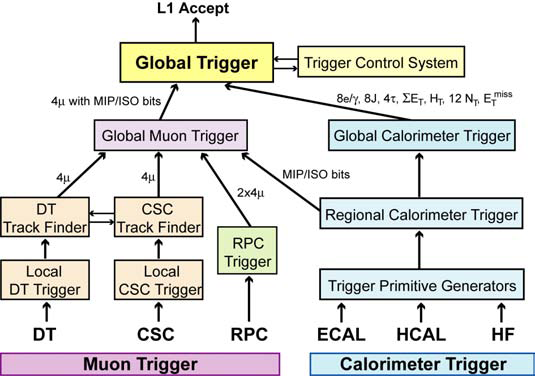
\includegraphics[width=0.95\textwidth]{figures/L1_architecture.png}
\caption{The architecture of the L1 Trigger.}
\label{fig:L1-trigger}
\end{center}
\end{figure}

The HLT further analyzes events which pass the L1A decision. Using a farm of roughly 1000 commercial processors comprised of over 13000 central processing units (CPUs), it emulates the full offline reconstruction algorithms described in Ch. \ref{ch:reconstruction}. Like the L1 Trigger, the HLT uses a set of triggers with different criteria, called the trigger menu. Different trigger menus are constructed for various conditions, including different instantaneous luminosity levels and different types of collisions or measurements. The selected menu can be changed during the operation of the detector in response to new conditions. Events which pass the HLT decision are sorted into primary datasets (PDs) with minimal overlap. The HLT output includes several streams, including monitoring and calibration streams in addition to the primary stream of physics events.

During the 2012 run, the L1 Trigger operated at rates up to 100\unit{kHz} with only 3\% dead time \cite{Brooke:2013hnf}. The HLT operated at rates up to 1\unit{kHz} and took an average of 200\unit{ms} to process an event \cite{Trocino:2014jya}. This processing speed is two orders of magnitude faster than the full offline reconstruction. The HLT achieves this fast processing time using several optimizations. The reconstruction algorithms in a given trigger path are arranged so that the fastest algorithms run first. If an algorithm's product does not pass a specified quality filter, the rest of the trigger path is skipped. In addition, the reconstruction algorithms only consider small regions of the detector output, based on the locations of L1 candidates.

\section{Luminosity Measurement
\label{sec:lumimeas}}

The fine resolution of the CMS pixel detector (Sec. \ref{sec:tracker}) implies that a given pixel will tend to be activated by one track at most per bunch crossing. A minimum bias interaction creates an average of 200 clusters, with each cluster containing an average of 5 pixels \cite{CMS-PAS-LUM-12-001}. Even with 100 pileup events per bunch crossing, the pixel detector will have an occupancy as low as 0.1\%. The number of pixel hits should thus scale linearly with the number of interactions per bunch crossing for instantaneous luminosities up to and even beyond the LHC design performance. Equation \eqref{eq:pixel-lumi} shows how the instantaneous luminosity $\mathcal{L}$ is related to the average number of pixel clusters per event $\langle n \rangle$ \cite{CMS-PAS-LUM-13-001}:
\begin{equation} \label{eq:pixel-lumi}
\mathcal{L} = \frac{\nu \langle n \rangle}{\sigma_\text{vis}}.
\end{equation}
Here, $\nu = 11246\unit{Hz}$ is the LHC revolution frequency, $\langle n \rangle$ is defined as $\mu n_{1}$ where $\mu$ is the number of collisions per bunch crossing and $n_{1}$ is the average number of clusters per collision, and the visible cross section $\sigma_\text{vis}$ is defined as $\sigma_\text{T} n_{1}$ where $\sigma_\text{T}$ is the total inelastic cross section. A Van der Meer scan \cite{Balagura:2011yw} is used to calibrate $\sigma_\text{vis}$. In 2012, CMS measured the total integrated luminosity with a systematic uncertainty of 2.6\% using this method.

The HF is used as a second method of measuring the luminosity. This is possible because the HF can be run safely during unstable beams \cite{CMS-PAS-LUM-13-001}. Information from the HF can be used to measure the luminosity in two different ways. The average fraction of empty towers can be related to the mean number of interactions per crossing, or the average transverse energy per tower can be linearly related to the luminosity. It can make an online determination of the average luminosity to a statistical uncertainty of 1\% in under 1\unit{s}. However, the calibration of this measurement can drift over long time periods due to changes in the gain of the HF PMTs. In practice, the increase in pileup interactions observed during the 2012 run moves the HF response into a nonlinear regime, limiting the accuracy of this method. Because of these limitations, the HF method is utilized primarily as a cross-check for the pixel cluster counting method.
\chapter{Event Reconstruction
\label{ch:reconstruction}}

Particles created in proton-proton collisions pass through the CMS detector and leave signals in different subdetectors. Figure \ref{fig:cms-slice} shows examples of typical signals for different types of particles. Each type of particle has a different characteristic signature from which it can be identified using information from the various subdetectors. Muons, electrons, and charged hadrons create tracks in the tracker, while photons and neutral hadrons do not. Muons also create hits in the muon systems. Electrons and photons deposit energy in the ECAL, while charged and neutral hadrons deposit most of their energy in the HCAL.

\begin{figure}[hbt]
\begin{center}
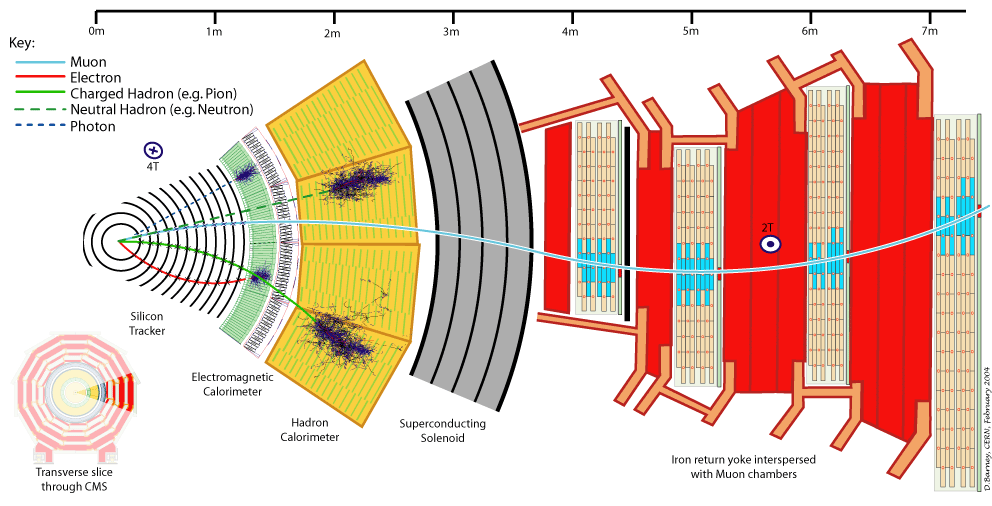
\includegraphics[width=0.95\textwidth]{figures/CMS_slice.png}
\caption{A cross-sectional view of the CMS detector with all subdetectors labeled and examples of signals left by muons, electrons, charged hadrons, neutral hadrons, and photons \cite{CMS-slice}.}
\label{fig:cms-slice}
\end{center}
\end{figure}

The raw output from each subdetector is processed in several steps in order to reconstruct the different types of particles \cite{TDR-software}. The first step is local reconstruction, which involves the creation of reconstructed hits or ``RecHits'' for each subsystem of each subdetector. The tracker RecHits include information about the positions of signals in the form of clusters, which are combinations of contiguous strips or pixels. The muon system RecHits also provide the positions of signals. In the DT and CSC subsystems, these RecHits can be combined into three-dimensional track segments. The ECAL and HCAL RecHits contain the energy, position, and time of energy deposits from traversing particles.

In the second step, global reconstruction, the RecHits from the different subsystems of a given subdetector are combined and further processed. In the tracker, pattern recognition algorithms are employed to reconstruct tracks for various cases, including displaced vertices, low \pt tracks, and high \pt tracks. The ECAL and HCAL RecHits are combined into calorimeter towers or ``CaloTowers'' using a projective $\eta$-$\phi$ geometry. ``Standalone'' muons are created by the muon system global reconstruction, which associates RecHits and track segments in a radial trajectory, accounting for bending by the residual magnetic field, and uses a vertex-constrained fit.

High-level reconstruction is the final step, in which information from all subdetectors is used to reconstruct various types of particles as precisely as possible. The particle types used in this search include electrons, muons, taus, jets, and b-jets. The reconstruction algorithms for these particles will be described in more detail in the following sections of this chapter. Many of these algorithms use a particle flow technique that is unique to CMS and will be described in Sec. \ref{sec:particle-flow}.

The CMS experiment uses detailed simulations to predict the performance of the detector and reconstruction algorithms and to model various physics processes. Each simulated event is generated from the interaction of partons in proton-proton collisions and the decays of the resulting particles, based on theoretical calculations. The traversal of the final state particles through the CMS detector is simulated to create simulated hits or ``SimHits''. The effects of photodetectors and readout electronics on these SimHits are also simulated. After that processing, the results can be treated identically to the raw data from real events and used as input for the reconstruction software.

\section{Event Generation}

\section{Detector Simulation}

\section{Tracks and Vertices
\label{sec:tracks}}

Hits from the different tracker subsystems are reconstructed into charged-particle tracks using the Combinatorial Track Finder (CTF) algorithm \cite{TrackingJINST}. CTF is an iterative algorithm which finds the easiest tracks first, in order to remove the associated hits from consideration. This reduces the complexity of finding more difficult tracks in subsequent iterations. Each iteration follows the same four-step procedure, varying the type of seed used and the selection criteria applied.
\begin{enumerate}
\item A seed is generated using only a few hits.
\item Additional hits are added to the track based on the extrapolated trajectory of the seed.
\item The parameters of the track are estimated using a fit which considers all hits in the trajectory.
\item Selection criteria are applied to determine the quality of the track, excluding those tracks which do not pass the selection.
\end{enumerate}

The types of seeds are categorized based on the number of hits included and the source of those hits. Initial iterations use pixel triplet and pair seeds, created from three and two pixel hits, respectively. These are the highest-quality seeds and are used to reconstruct prompt tracks, those emitting from primary vertices near the IP. A subsequent iteration uses a mixed triplet seed, containing 1--3 pixel hits and ${<}3$ strip hits. This iteration typically finds displaced tracks from heavy flavor decays, nuclear interactions, and photons which convert to \EpEm\xspace pairs in the tracker. The final iterations use strip pair seeds, consisting of two matched hits from the strip detectors, usually generated by charged particles which did not enter the pixel detector.

The iterations that use seeds with strip hits may also find prompt tracks which lack pixel hits. The specific sequence of iterations has been modified several times to improve the computing and physics performance of CMS tracking \cite{Tracking2012}. Table \ref{tab:tracking} lists the sequence used during the 2012 run. The selection criteria for each iteration are given, including cuts on \pt, transverse impact parameter $d_0$, and longitudinal impact parameter $z_0$. Some of the $z_0$ cuts are in terms of $\sigma$, the length of the beam spot in the $z$-direction used as a Gaussian standard deviation.

\begin{table}[htb]
  \begin{center}
    \begin{tabular}{llllll}
\hline
step  & seed type & seed subdetectors & \pt $[\GeVcns]$ & $d_0$ [cm] & $|z_0|$ \\
\hline
0     & triplet   & pixel             & ${>}0.6$     & ${<}0.02$  & ${<}4.0\sigma$ \\
1     & triplet   & pixel             & ${>}0.2$     & ${<}0.02$  & ${<}4.0\sigma$ \\
2     & pair      & pixel             & ${>}0.6$     & ${<}0.015$ & ${<}0.09\cm$ \\
3     & triplet   & pixel             & ${>}0.3$     & ${<}1.5$   & ${<}2.5\sigma$ \\
4     & triplet   & pixel/TIB/TID/TEC & ${>}0.5$--0.6 & ${<}1.5$   & ${<}10.0\cm$ \\
5     & pair      & TIB/TID/TEC       & ${>}0.6$     & ${<}2.0$   & ${<}10.0\cm$ \\
6     & pair      & TOB/TEC           & ${>}0.6$     & ${<}2.0$   & ${<}30.0\cm$ \\
\hline
    \end{tabular}
    \caption{The sequence of tracking iterations used during the 2012 run, including information on the seeds and selection criteria used in each step \cite{Tracking2012}.}
    \label{tab:tracking}
  \end{center}
\end{table}

The reconstructed tracks are used to reconstruct the primary vertices from the event \cite{TrackingJINST}. This includes both the main hard scatter vertex and additional vertices from pileup collisions. First, selection requirements are imposed on the tracks, in order to consider only prompt tracks near the IP. The selection requirements include cuts on the significance of $d_0$, the number of pixel and strip hits in the track, and the normalized $\chi^2$ from the fit of the track trajectory. The tracks which pass the selection requirements are clustered together using their $z$-coordinates, determined at each track's closest approach to the beam spot. A deterministic annealing algorithm is used to perform this clustering, in which each track may have a different probability to be associated with each vertex. The algorithm uses analogues of statistical mechanics quantities, slowly reducing the ``temperature'' and minimizing the ``free energy'' during each temperature iteration.

Once the deterministic annealing algorithm produces a list of vertex candidates, an adaptive vertex fitter is applied to each vertex candidate. This fitter weights each track in the vertex based on the agreement between the track and vertex positions. Using those weights, it fits the parameters of the vertex, including the $(x,y,z)$ position, the covariance matrix, and the number of degrees of freedom, $n_{\text{dof}} = -3 + 2 \sum{w_i}$, where $w_i$ is the weight for the $i$th track. The variable $n_{\text{dof}}$ can be used to select vertices which correspond to actual proton-proton interactions, as it is closely related to the number of tracks compatible with the vertex.

%add 2012 performance (efficiency, fake rate, vtx resolution)? references only have 2011 performance...

\section{Particle Flow
\label{sec:particle-flow}}

The CMS experiment uses a technique called particle flow (PF) to combine information from all subdetectors in order to identify all stable particles in each event \cite{CMS-PAS-PFT-09-001}. As described at the beginning of this chapter and shown in Fig. \ref{fig:cms-slice}, each type of stable particle is expected to create signals in a certain subset of the subdetectors. The performance of the PF algorithm was validated using early CMS data \cite{CMS-PAS-PFT-10-002,CMS-PAS-PFT-10-003}, along with newer CMS data for more recent uses of the algorithm \cite{Beaudette:2014cea}, demonstrating significant improvement over simpler approaches. The reconstructed particles are known as PF candidates, which can be treated as input particles by the various high-level reconstruction algorithms. PF candidates can also be used to compute the isolation of a reconstructed object, by summing the energy of candidates topologically close to the selected object.

The RecHits from the local reconstruction process are used to create the basic elements for this technique: tracks and clusters. Charged-particle tracks are created from tracker RecHits using an iterative algorithm as described in Sec. \ref{sec:tracks}, and muon tracks are created from muon system RecHits. Calorimeter energy deposits are grouped into clusters by identifying seed hits as local energy maxima exceeding a certain threshold, and then adding neighboring hits with energy above subsystem-specific thresholds meant to eliminate photodetector noise. Further removal of noise from the calorimeters is performed by rejecting clusters with characteristics matching those expected from leading sources of noise. Tracks and clusters are associated together using a linking algorithm that determines if they were likely produced by the same particle. The algorithm considers a possible link between each algorithm based on the $\eta$-$\phi$ distance between a charged-particle track and a cluster, or between two clusters. For links between a charged-particle track and a muon track, the $\chi^{2}$ value from a global fit is used as the link distance. Groups of elements are associated based on minimizing the link distance and are called ``blocks''.

PF reconstruction algorithms classify the blocks as different types of particles. When a block is classified as a certain type of particle, it is removed from the list of unclassified blocks. A global muon block is accepted as a PF muon if the momentum of the combined charged-particle and muon tracks agrees with the momentum of the charged-particle track alone. The energy expected to have been deposited by the PF muons in the calorimeters due to minimum ionization is subtracted from the clusters. The remaining charged-particle tracks are checked for compatibility with electrons, which tend to leave short tracks and radiate energy via bremsstrahlung. A Gaussian Sum Filter (GSF) is applied to the compatible tracks in order to identify spatially-matched ECAL clusters, and the combination of a track and one or more clusters is classified as a PF electron.

The remaining tracks are linked to clusters to form PF charged hadrons, if the total cluster energy is similar to but smaller than the total track momentum. More than one track can link to a given cluster, but for a given track, only the link to the closest cluster is kept. This reflects the coarser segmentation of the calorimeter system as compared to that of the tracker. In cases where the total cluster energy is significantly smaller than the total track momentum, additional PF muons may be found using tracks from the block, and some tracks may be classified as fake and removed from consideration. Finally, an excess of energy in the clusters, above the total track momentum, is assumed to come from neutral particles. The excess energy is typically classified as a PF photon. If the total excess cluster energy in a block is larger than the total ECAL energy in the cluster, a PF neutral hadron is created from the excess energy remaining after assigning the ECAL excess energy to a PF photon. The remaining clusters not linked to any tracks are used to create PF photons in ECAL and PF neutral hadrons in HCAL.

\section{Electrons}

\section{Muons}

\section{Taus}

\section{Jets}

\section{b-tagging}
\chapter{Data Analysis
\label{ch:analysis}}

\section{Data Samples}

\subsection{Observed Data}

\subsection{Monte Carlo}

\section{Selection and Optimization}

\subsection{Object Identification}

\subsubsection{Muons
\label{sec:muon-obj}}

Two working points for the quality cuts described in Sec. \ref{sec:muon-reco} are used to identify reconstructed muons. Table \ref{tab:muonWP} lists the various requirements in each working point. The leading muon in the \mutau channel is selected with the tight working point; in addition to those quality cuts, it is required to have $\pt>30\GeV$ and $|\eta|<2.1$ to match the specifications of the HLT criterion used to collect the primary dataset. The loose working point is used to veto additional muons and for selections in some control regions. Less restrictive kinematic cuts $\pt>20\GeV$ and $|\eta|<2.4$ are applied to muons identified with the loose working point.

\begin{table}[htb]
  \begin{center}
    \begin{tabular}{|l|l|}
\hline
\multicolumn{2}{|c|}{Working Point}\\
\hline
\multicolumn{1}{|c|}{Tight} & \multicolumn{1}{c|}{Loose} \\
\hline
PF muon & PF muon \\
Global muon & Global muon OR tracker muon \\
$\begin{aligned}
I^{\text{PF}}_{\mu}/\pt &< 0.12 \\
d_0 &< 0.2\cm \\
d_z &< 0.5\cm \\
\text{Global track fit } \chi^2/n_{\text{dof}} &< 10 \\
\text{Global track fit } n_{\text{muon segment}} &> 0 \\
n_{\text{hits}}(\text{pixel}) &> 0 \\
n_{\text{layers}}(\text{tracker}) &> 5 \\
n_{\text{stations}}(\text{muon}) &> 1
\end{aligned}$
&
$\begin{aligned}
I^{\text{PF}}_{\mu}/\pt &< 0.3 \\
\\
\\
\\
\\
\\
\\
\\
\end{aligned}$ \\
\hline
    \end{tabular}
    \caption{The quality cuts for the tight and loose working points of the muon identification.}
    \label{tab:muonWP}
  \end{center}
\end{table}

\subsubsection{Electrons
\label{sec:ele-obj}}

Two working points for the quality cuts described in Sec. \ref{sec:ele-reco} are used to identify reconstructed electrons. Electrons are considered to be in the barrel if they have $|\eta|<1.444$ and in the endcap if they have $1.56<|\eta|<2.5$. Table \ref{tab:eleWP} lists the various requirements in each working point. The leading electron in the \etau channel is selected with the medium working point; in addition to those quality cuts, it is required to have $\pt>30\GeV$ to match the specifications of the HLT criterion used to collect the primary dataset. The loose working point is used to veto additional electrons and for selections in some control regions. The less restrictive kinematic cut $\pt>20\GeV$ is applied to electrons identified with the loose working point.

\begin{table}[htb]
  \begin{center}
    \begin{tabular}{|r|c|c|c|c|}
      \hline
      \multirow{3}{*}{Cut Variable} & \multicolumn{4}{|c|}{Cut Value} \\
      \cline{2-5}
                                    & \multicolumn{2}{|c|}{Medium} & \multicolumn{2}{|c|}{Loose} \\
      \cline{2-5}
                                    & Barrel & Endcap & Barrel  & Endcap    \\
      \hline
      $I^{\text{PF}}_{\Pe}/\pt<$    & 0.15     & 0.15     & 0.15      & 0.15      \\      
      $\sigma_{i\eta i\eta}<$       & 0.01     & 0.03     & 0.01      & 0.03    \\ 
      $|\Delta\phi_{\text{in}}|<$   & 0.06     & 0.03     & 0.15      & 0.10    \\ 
      $|\Delta\eta_{\text{in}}|<$   & 0.004    & 0.007    & 0.007     & 0.009    \\ 
      $H/E<$                        & 0.12     & 0.10     & 0.12      & 0.10     \\ 
      $|d_0^{\text{vtx}}|<$         & 0.02     & 0.02     & 0.02      & 0.02     \\              
      $|d_z^{\text{vtx}}|<$         & 0.1      & 0.1      & 0.2       & 0.2      \\              
      $|1/E - 1/p|<$                & 0.05     & 0.05     & 0.05      & 0.05     \\
      \hline
    \end{tabular}
    \caption{The quality cuts for the medium and loose working points of the electron identification. }
    \label{tab:eleWP}
  \end{center}
\end{table}

\subsubsection{Taus
\label{sec:tau-obj}}

Reconstructed hadronically decaying tau leptons are identified using the various discriminators defined in Sec. \ref{sec:hpstau}. Different working points for each discriminator are used in each channel, as listed in Table \ref{tab:tauWP}. In addition to these discriminators, each reconstructed tau lepton is required to have $\pt>30\GeV$ and $|\eta|<2.3$.

\begin{table}[htb]
  \begin{center}
    \begin{tabular}{|c|c|c|}
      \hline
      \multirow{2}{*}{Discriminator} & \multicolumn{2}{|c|}{Working Point} \\
      \cline{2-3}
                                    & \etau & \mutau \\
      \hline
      Isolation                     & Loose (3 hits)   & Loose (3 hits) \\
      anti-\Pe                      & Loose MVA (v3)   & Loose MVA (v3) \\
      anti-$\mu$                    & Loose (v2)       & Tight (v2) \\
      \hline
    \end{tabular}
    \caption{The working points for the different tau discriminators used in the tau lepton identification. }
    \label{tab:tauWP}
  \end{center}
\end{table}

\subsubsection{Jets
\label{sec:jet-obj}}

The loose working point of the PF jet identification algorithm is used to identify reconstructed jets. The requirements for the loose working point are summarized in Table \ref{tab:jetWP}. To eliminate jets from pileup interactions, each selected jet is required to have $\pt>30\GeV$. The cut $|\eta|<2.4$ is also applied, in order to include only jets measured in the best-performing regions of the detector. To select b-tagged jets, the discriminator calculated by the CSV algorithm is required to have a value greater than 0.244. This is the loose working point of the CSV algorithm, which limits the misidentification probability to 10\%.

\begin{table}[htb]
  \begin{center}
    \begin{tabular}{|r|c|}
      \hline
      \multirow{2}{*}{Cut Variable} & Cut Value \\
      \cline{2-2}
                                    & Loose \\
      \hline
      $f_{\text{CH}}>$              & 0.0 \\
      $f_{\text{NH}}<$              & 0.99 \\
      $f_{\gamma}<$                 & 0.99 \\
      $f_{\text{EM}}<$              & 0.99 \\
      $n_{\text{charged}}>$         & 0 \\
      $n_{\text{constituents}}>$    & 1 \\
      \hline
    \end{tabular}
    \caption{The quality cuts for the loose working point of the jet identification. }
    \label{tab:jetWP}
  \end{center}
\end{table}

\subsubsection{Primary Vertices
\label{sec:vtx-obj}}

Several requirements are applied to the reconstructed primary vertices to ensure high quality \cite{CMS-PAS-TRK-10-005}. The number of degrees of freedom $n_{\text{dof}}$, defined in Sec. \ref{sec:tracks}, must be greater than 4. The longitudinal position $z$ of the vertex must obey $|z|<24\mm$, and the transverse position $\rho$ must obey $|\rho|<2\mm$. In addition, the vertex must be reconstructed by a fit to tracks. The other reconstructed objects described above can be assigned to a reconstructed vertex. The closest vertex to the track associated with the object is chosen as its vertex. For electrons, the GSF track is used; for muons, the Best Track is used; and for hadronic tau leptons, the track of the leading charged hadron is used.

\section{Selection and Optimization}

The events analyzed in this dissertation are selected based on requirements for the numbers and types of different reconstructed objects and the relationships between those objects within each event. The selection criteria are applied in three stages. The most basic criteria are applied first in the preselection. This stage is used to validate the Monte Carlo background simulations by examining various relevant kinematic distributions. Second, additional criteria are applied in the main selection, which more closely addresses the expected properties of signal events. Kinematic distributions in the main selection are used to optimize the cuts for the final selection, in order to reduce the contributions from background while enhancing the signal. These optimizations maximize the expected limit from the MC background simulations. Separate final selections are defined for the leptoquark search and the top squark search.

\subsection{Preselection}

At the preselection stage, a single primary well-identified light lepton $\ell$ is required. In the \etau channel, this is an electron satisfying the medium working point and kinematic criteria described in Sec. \ref{sec:ele-reco}. In the \mutau channel, this is a muon satisfying the tight working point and kinematic criteria described in Sec. \ref{sec:muon-reco}. In addition to the light lepton, the event must contain a hadronic tau identified by the HPS algorithm and associated discriminators as defined in Sec. \ref{sec:hpstau}. The two objects, light lepton and hadronic tau, must have opposite charges, originate from the same vertex, and be separated by $\Delta R > 0.5$. Two jets are also required, satisfying the loose working point and kinematic criteria described in Sec. \ref{sec:jet-reco}. The jets must be separated from the light lepton and the hadronic tau by $\Delta R > 0.5$.

Several cases of additional light leptons are vetoed. To suppress background from the \Z+jets process, events are rejected if they contain additional light leptons satisfying the loose working point and having the same flavor and opposite charge with respect to the primary lepton. This separates the contributions from the $\Z \rightarrow \ell\ell$+jets process into control regions which will be used for background estimation. To avoid overlap between the two channels, events are rejected if they contain additional light leptons satisfying the primary working point and kinematic criteria for leptons (medium for electrons and tight for muons) and having the opposite flavor and opposite charge with respect to the primary lepton. This also defines an \emu control region which will be used for background estimation.

Figures \ref{fig:preseletau} and \ref{fig:preselmutau} compare the observed data to the MC background simulation after the preselection in the \etau and \mutau channels, respectively. All histograms in this dissertation show the overflow, if any, in the last bin. The event yields for the observed data and the expected SM backgrounds after the preselection are summarized in Table \ref{tab:eventyieldpresel}. The discrepancy between the observed data and simulated background yields in the \etau channel is due to the presence of QCD multijet events in the observed data. This discrepancy is primarily observed at low \pt and high $\eta$, as expected from QCD. This process is not modeled in the MC simulation because of the difficulty in simulating enough events to be comparable to the amount of data collected by the CMS experiment in 2012. Instead, the yield from QCD is estimated using a same-sign/opposite-sign method which is described in detail in Sec. \ref{??}.

\begin{figure}[hbtp]
  \begin{center}
    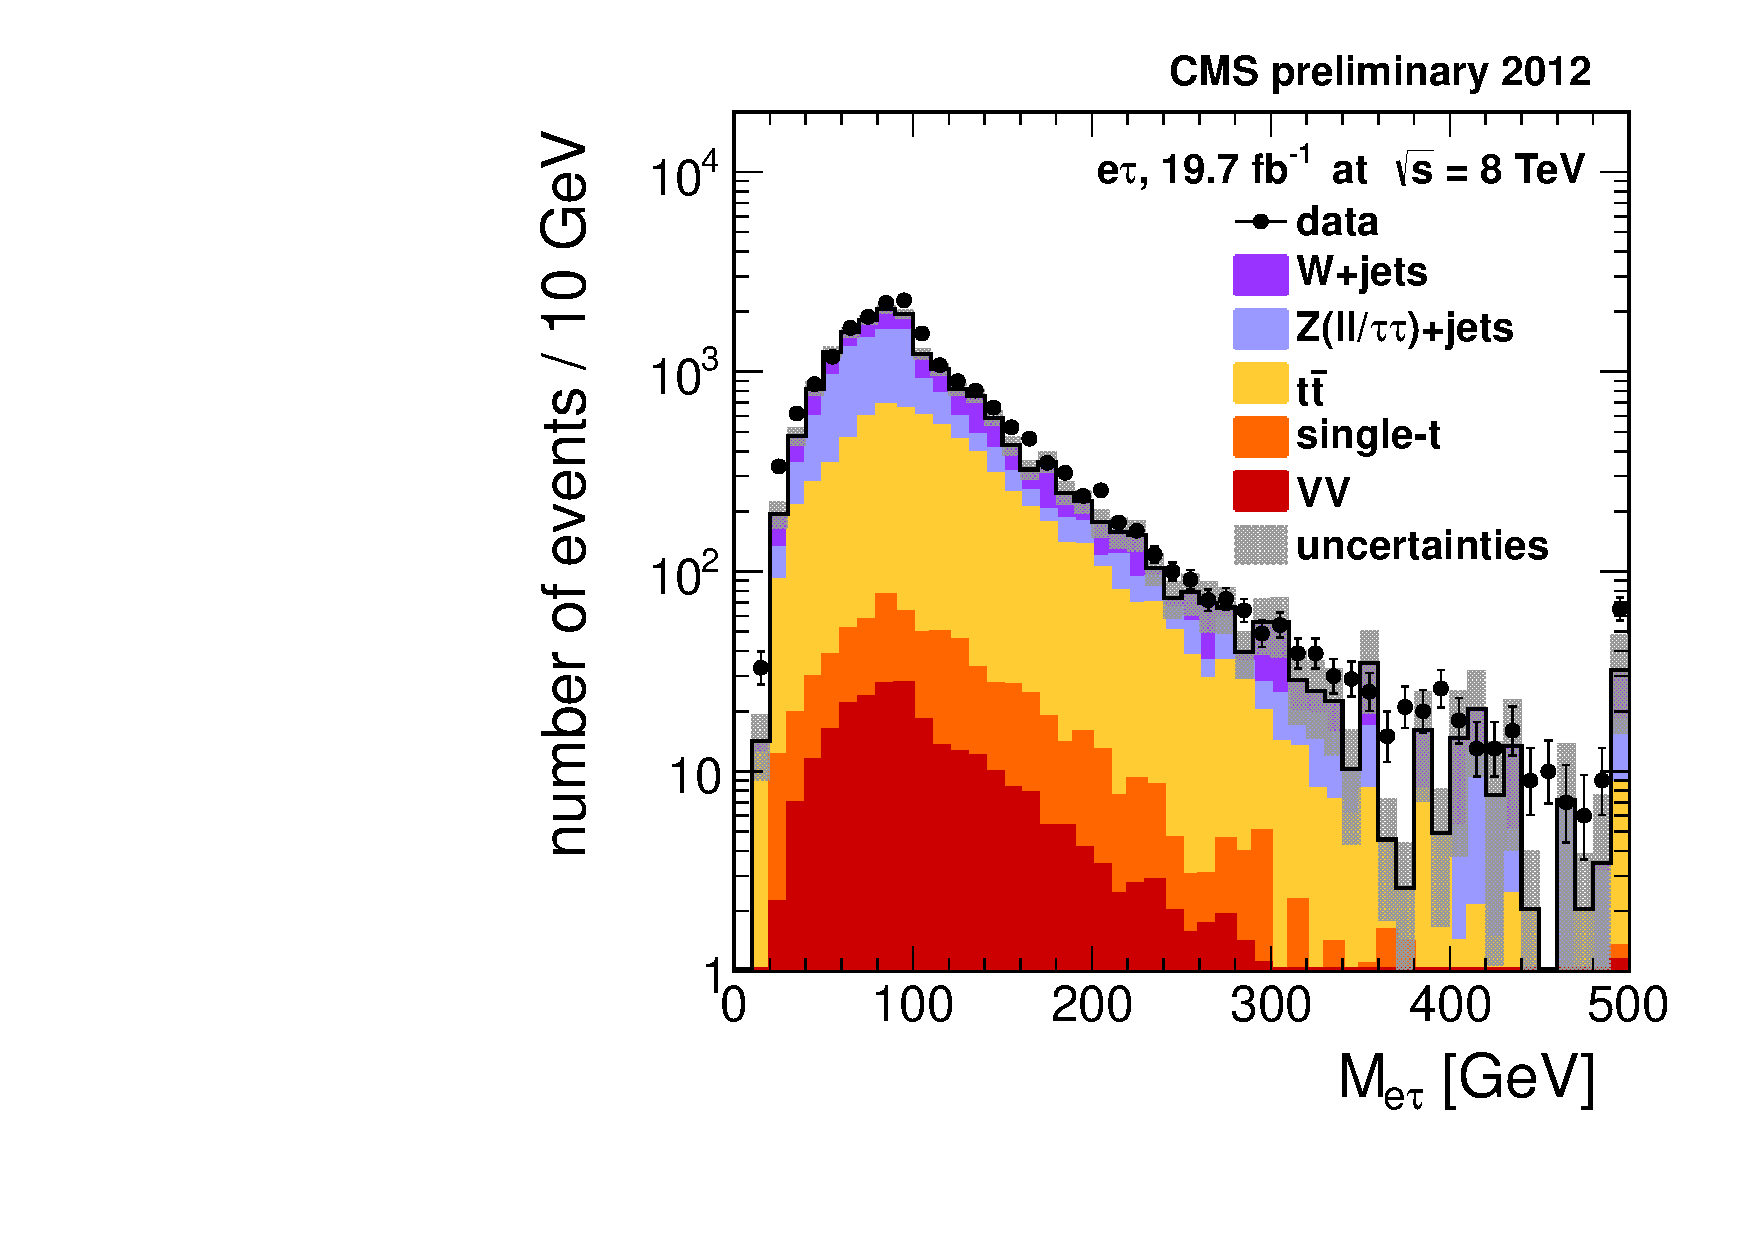
\includegraphics[width=0.465\textwidth]{figures/etau/etauMassMultJet.pdf}
    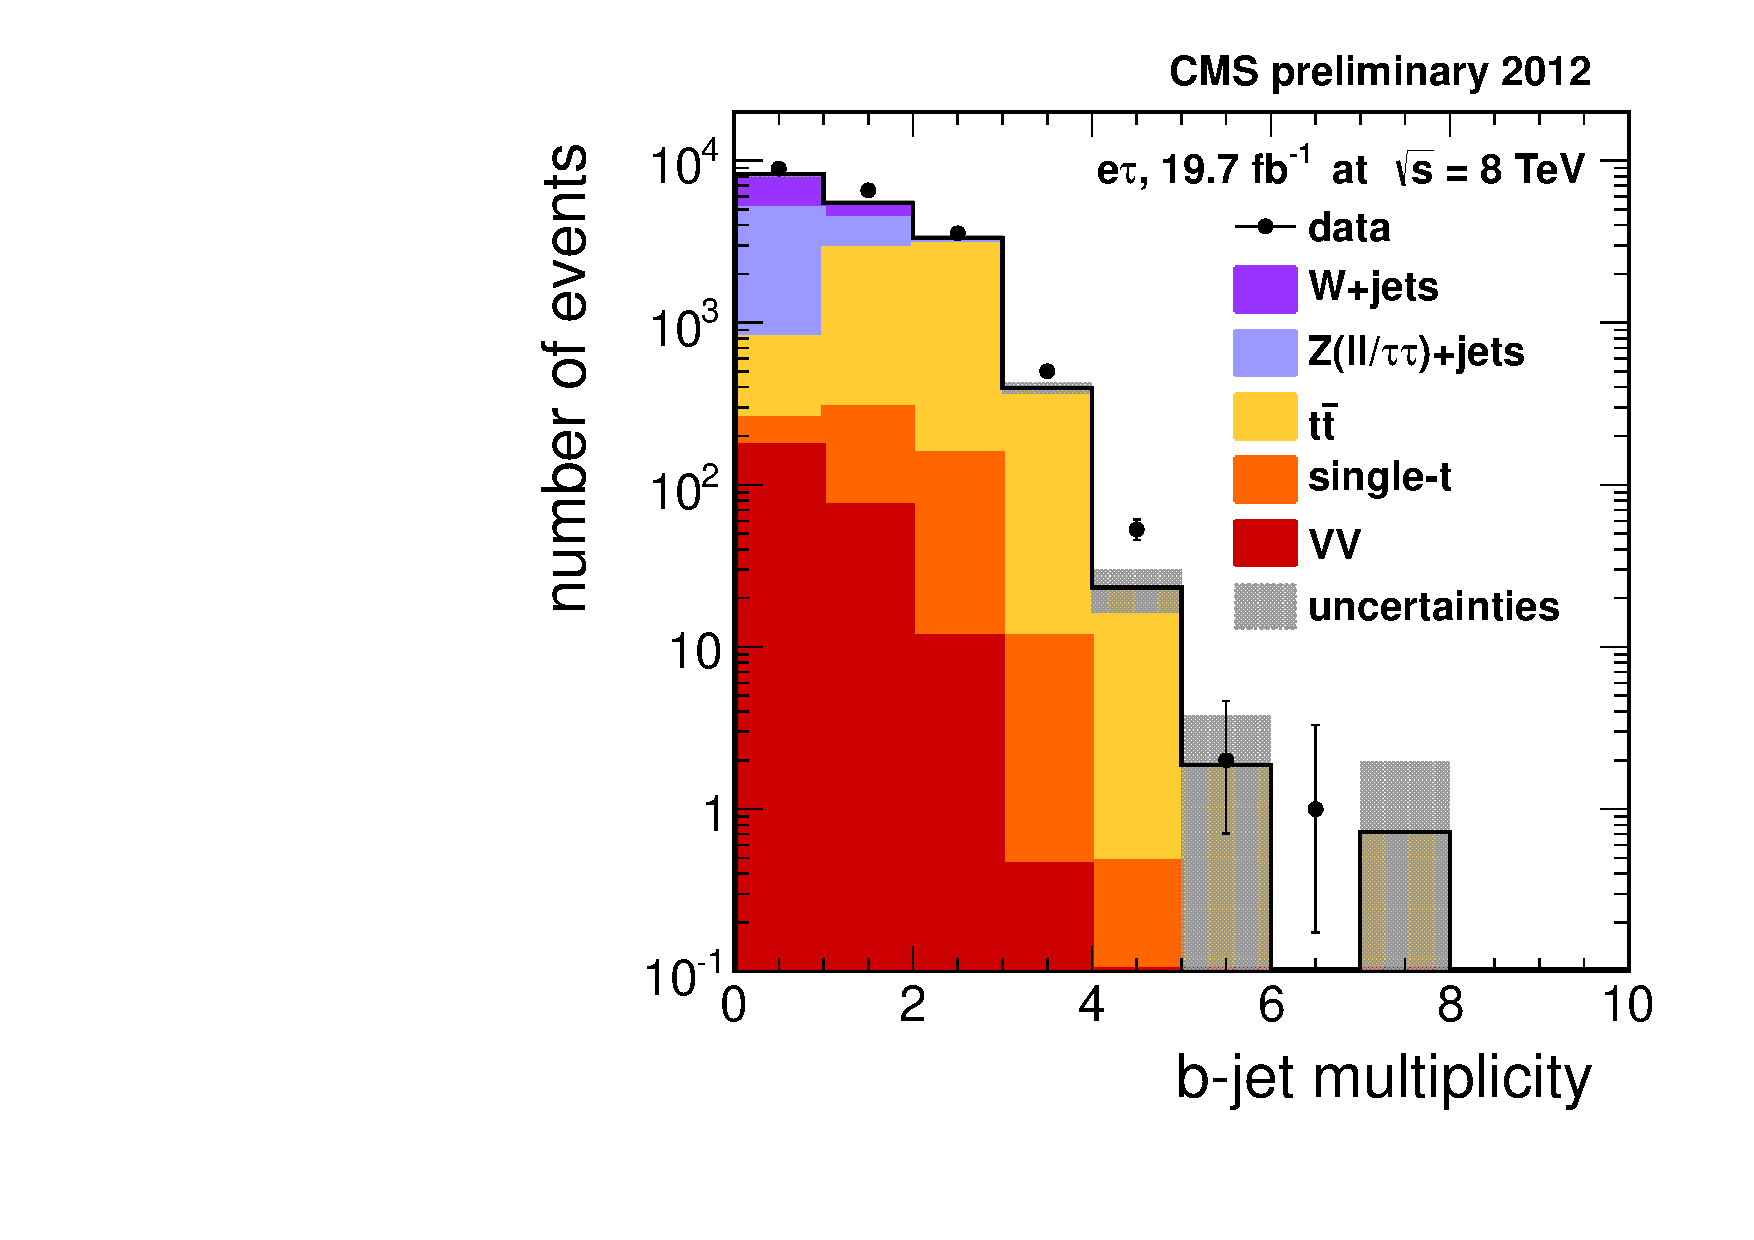
\includegraphics[width=0.465\textwidth]{figures/etau/nBJetMultJet.pdf} \\
    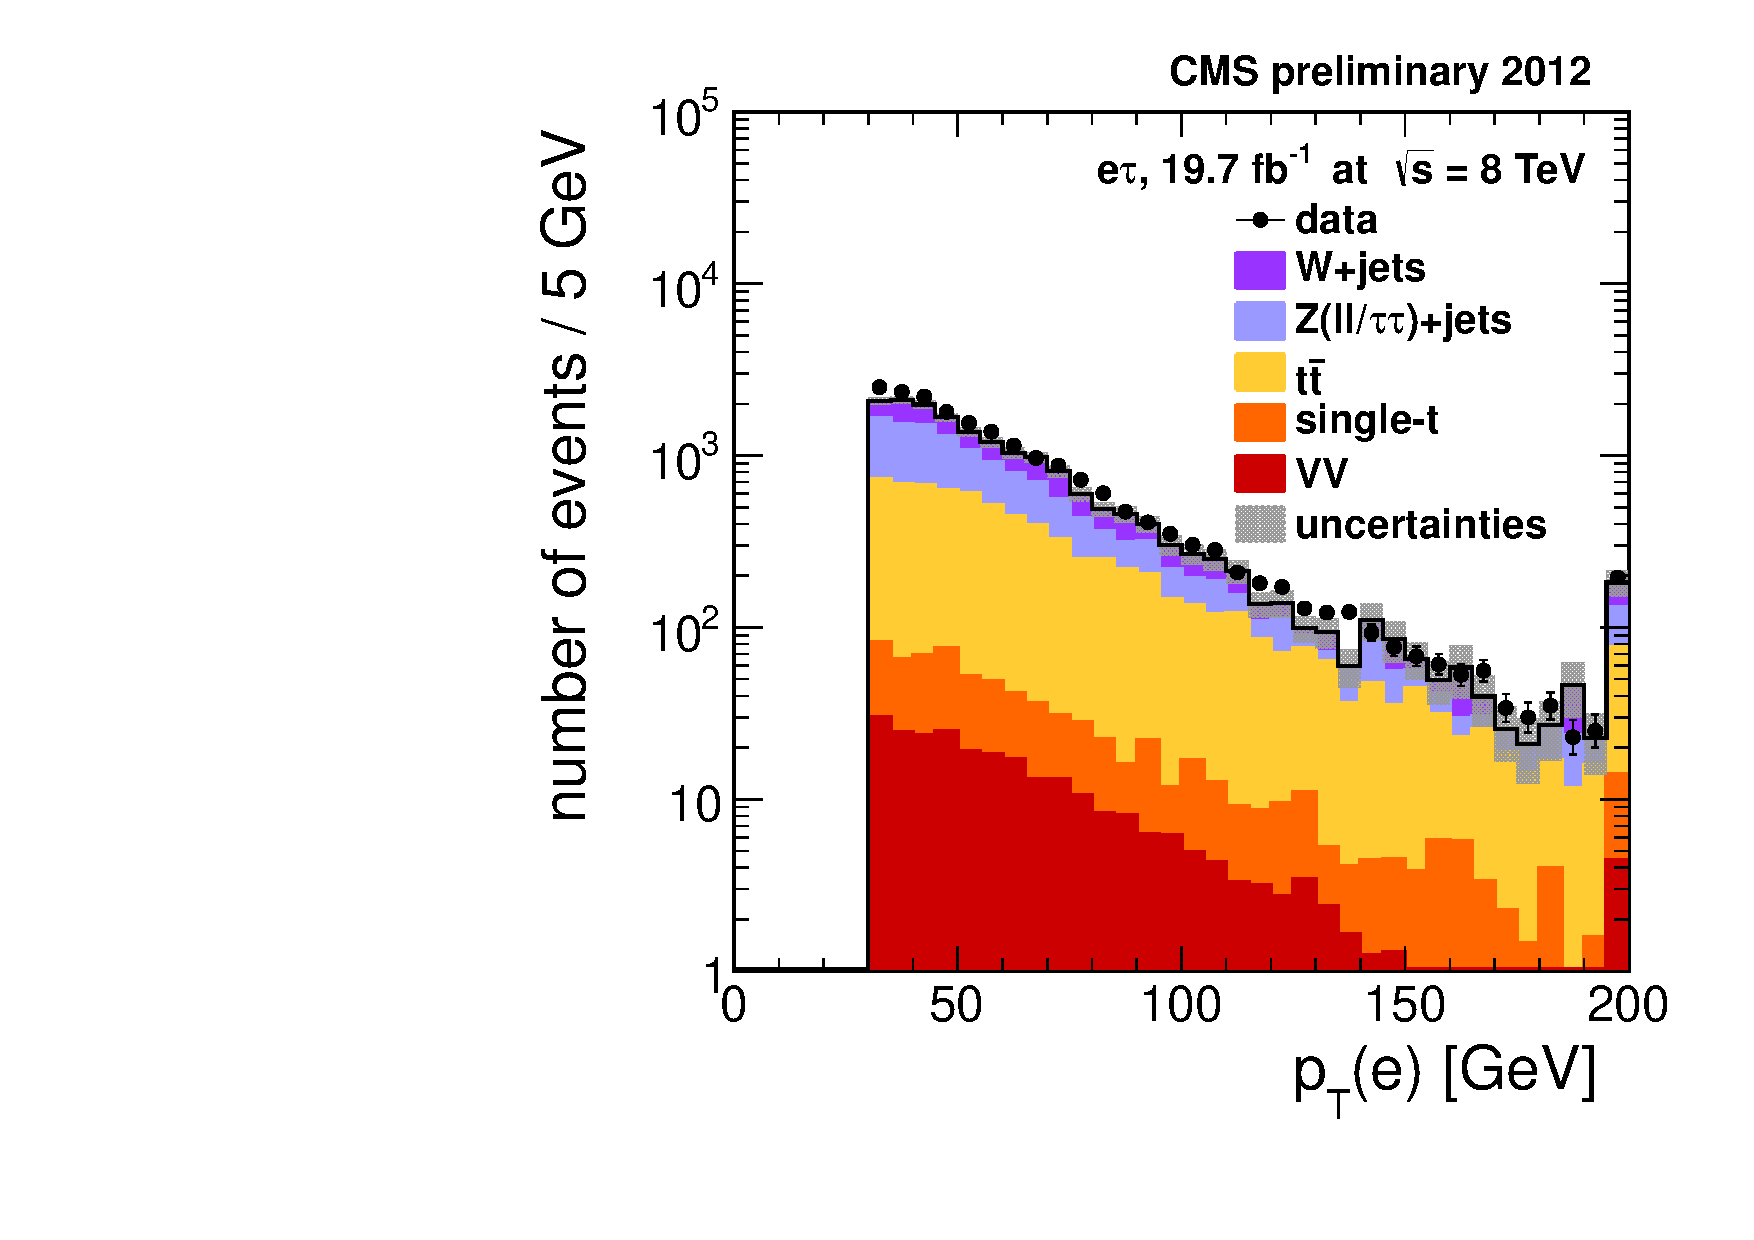
\includegraphics[width=0.465\textwidth]{figures/etau/elPtMultJet.pdf}
    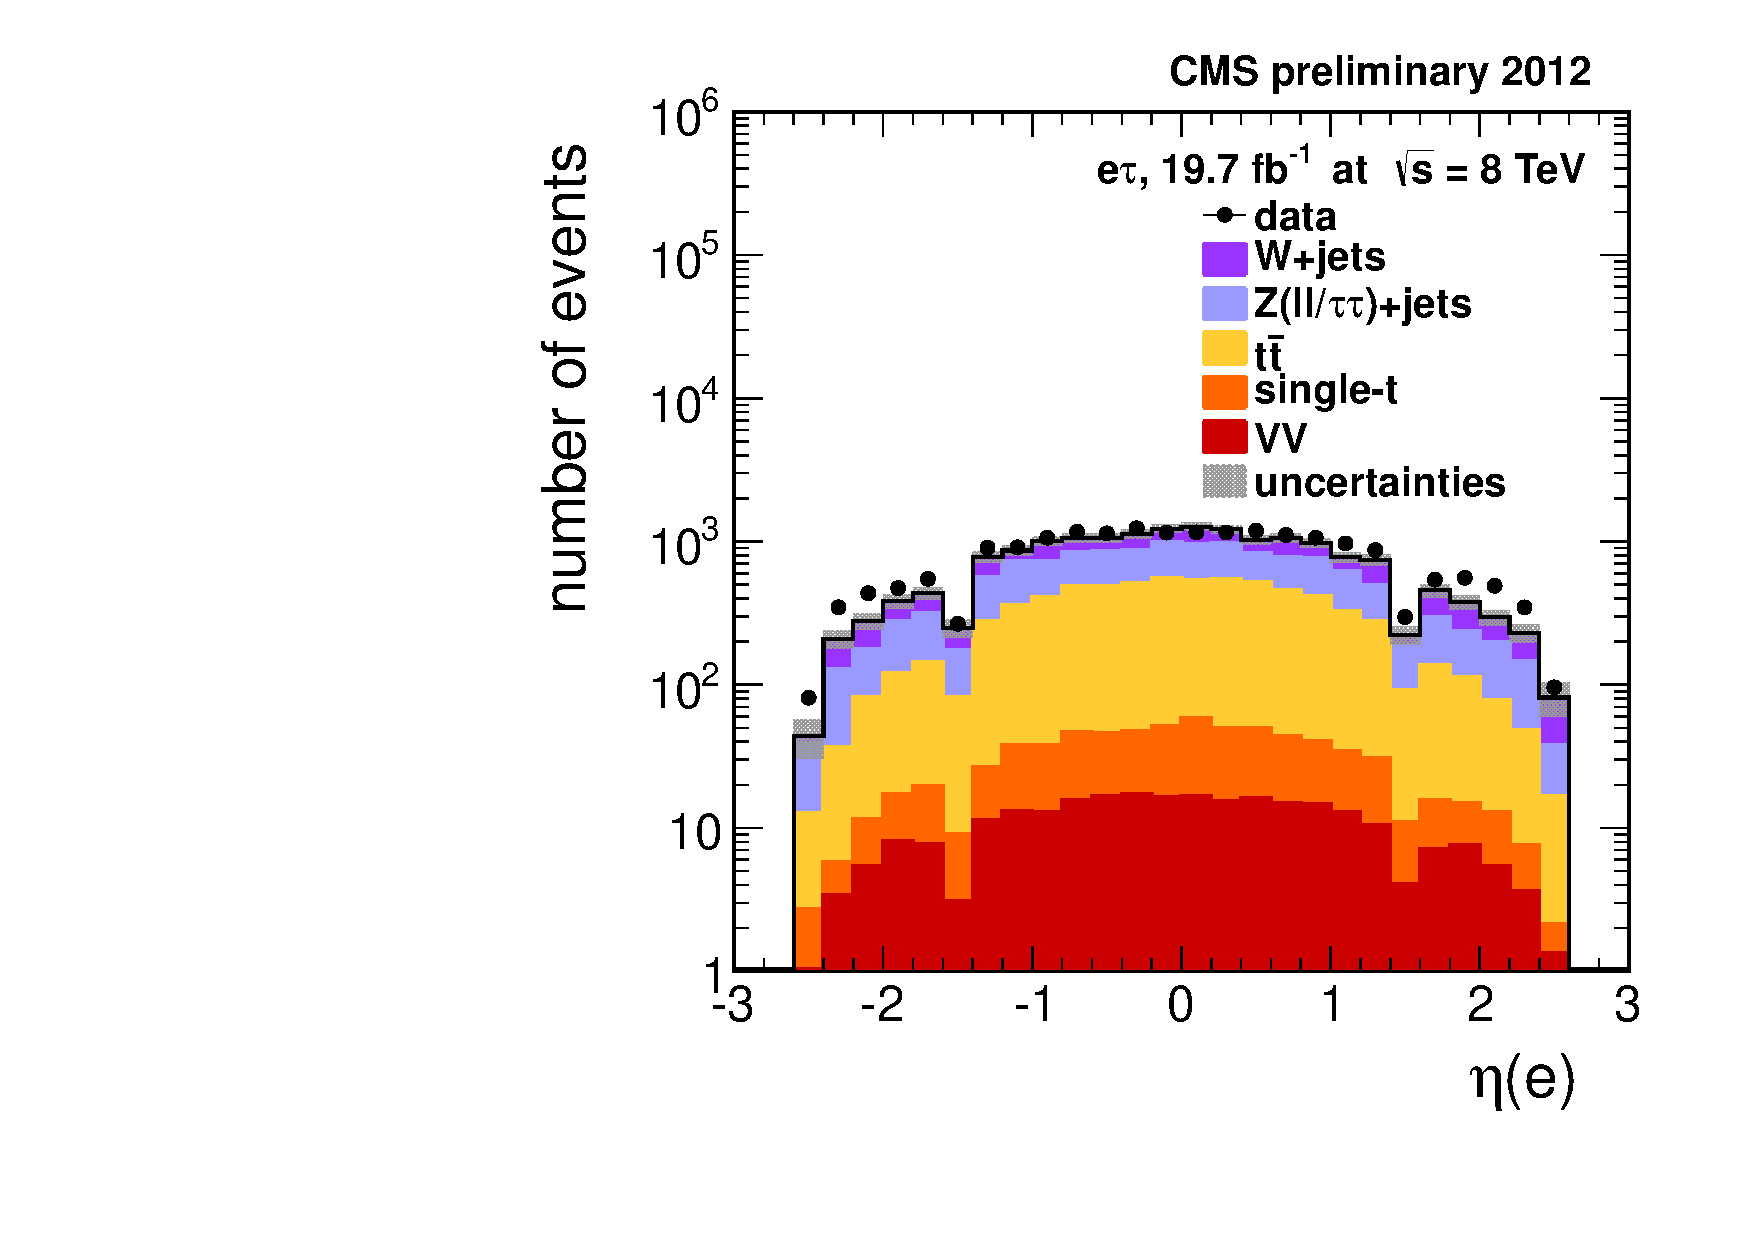
\includegraphics[width=0.465\textwidth]{figures/etau/elEtaMultJet.pdf} \\
    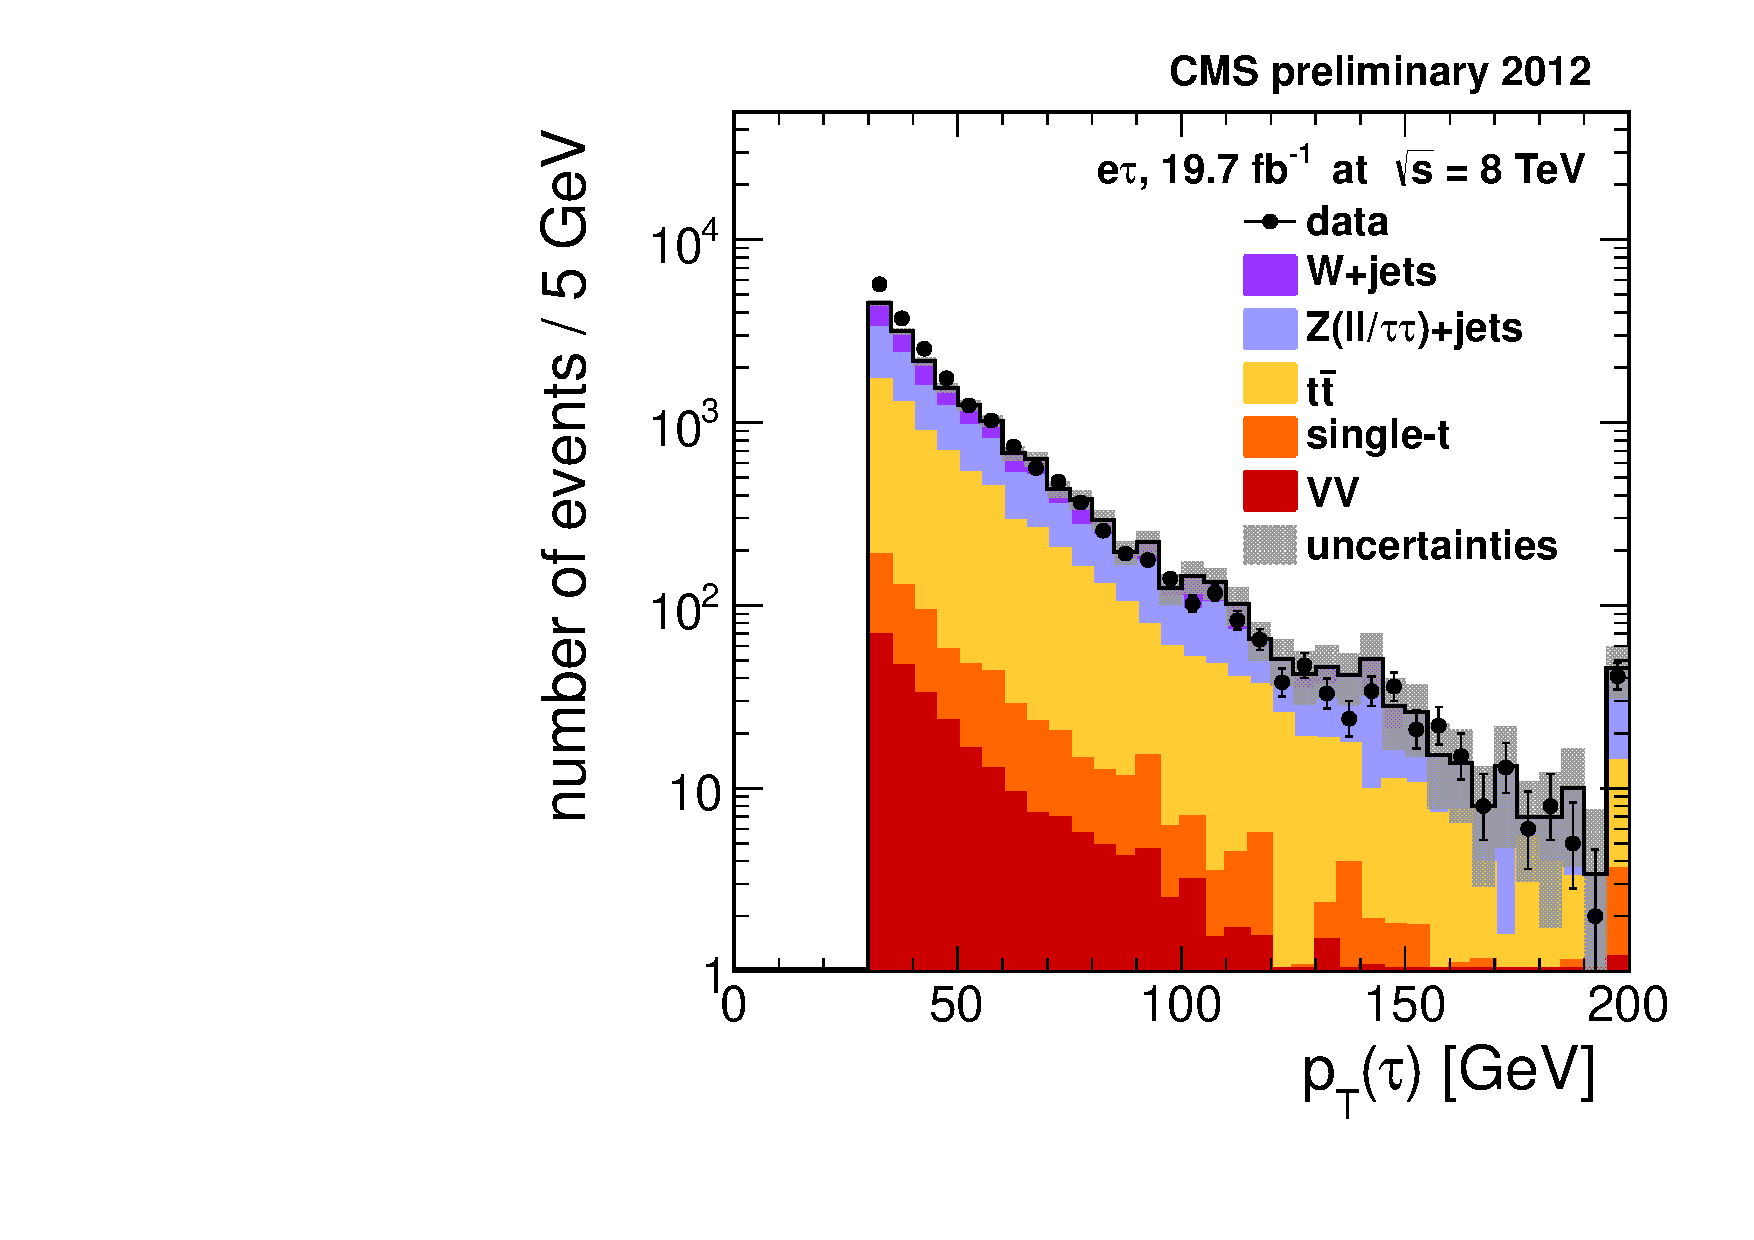
\includegraphics[width=0.465\textwidth]{figures/etau/tauPtMultJet.pdf}
    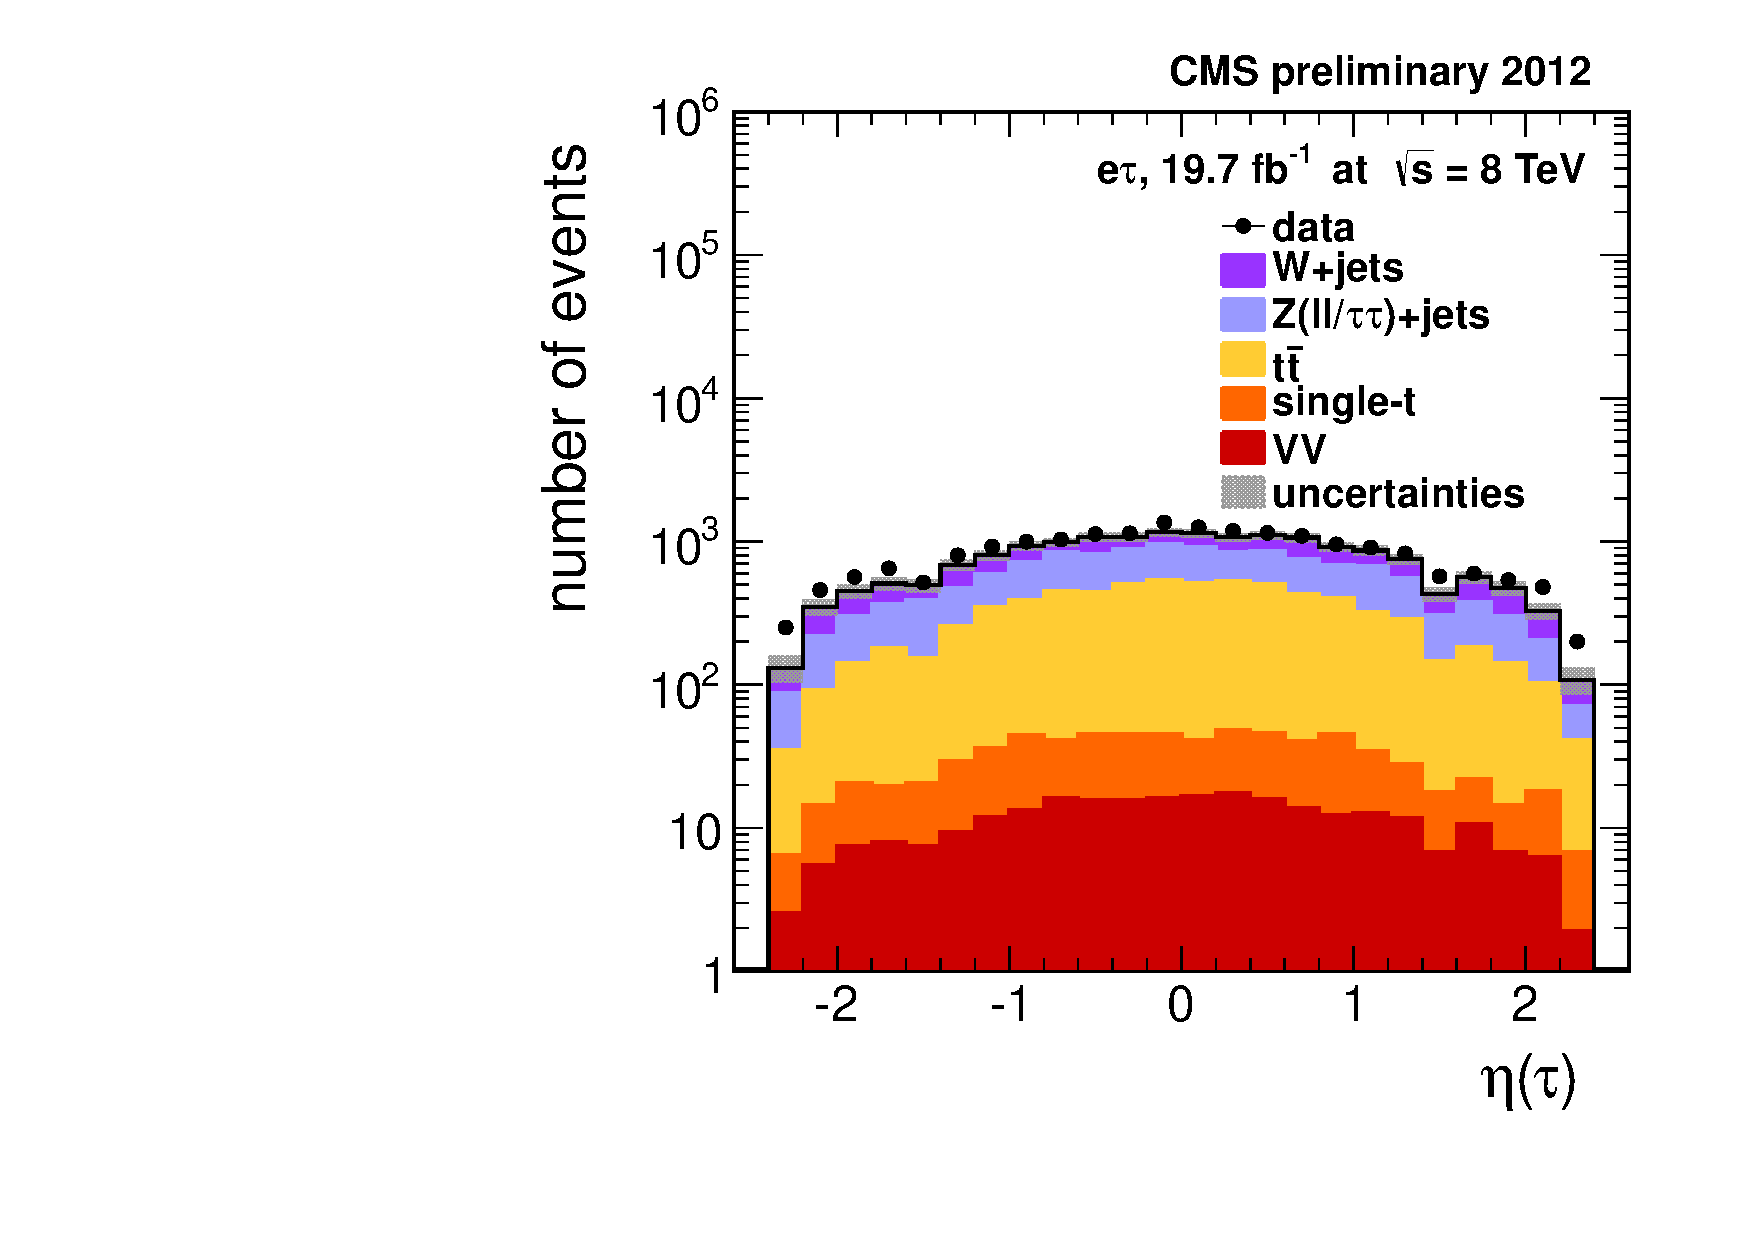
\includegraphics[width=0.465\textwidth]{figures/etau/tauEtaMultJet.pdf}
    \caption{Plots of various kinematic quantities comparing observed data and simulated backgrounds in the \etau channel after the preselection: the visible mass of the electron and hadronic tau (top left), the number of b-tagged jets (top right), the \pt (left) and $\eta$ (right) of the electron (middle) and hadronic tau (bottom). The uncertainty band reflects the statistical uncertainty in the simulated backgrounds.}
    \label{fig:preseletau}
  \end{center}
\end{figure}

\begin{figure}[hbtp]
  \begin{center}
    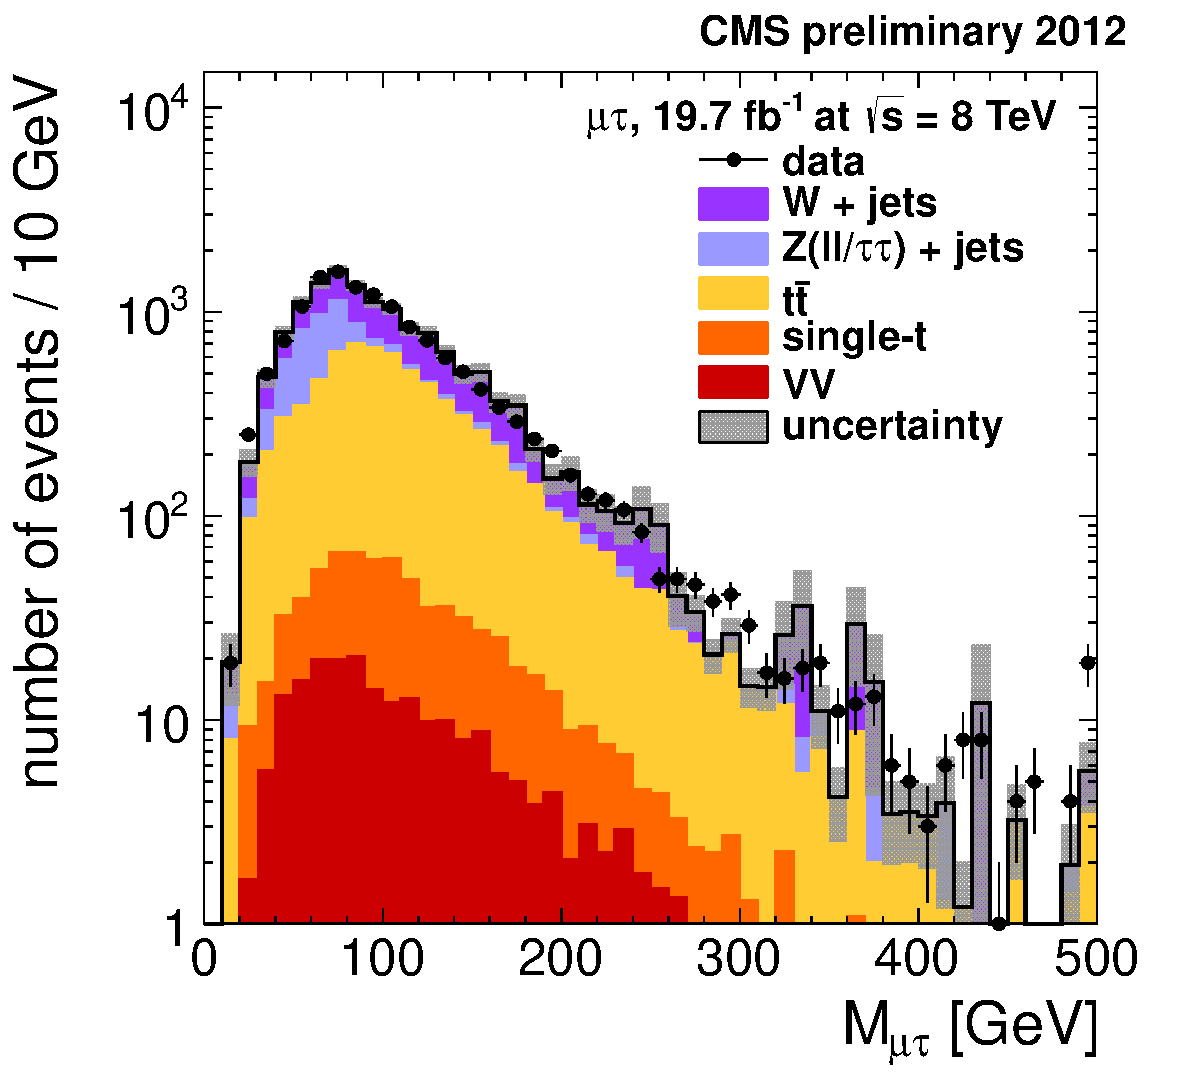
\includegraphics[width=0.465\textwidth]{figures/mutau/preselection/mass.pdf}
    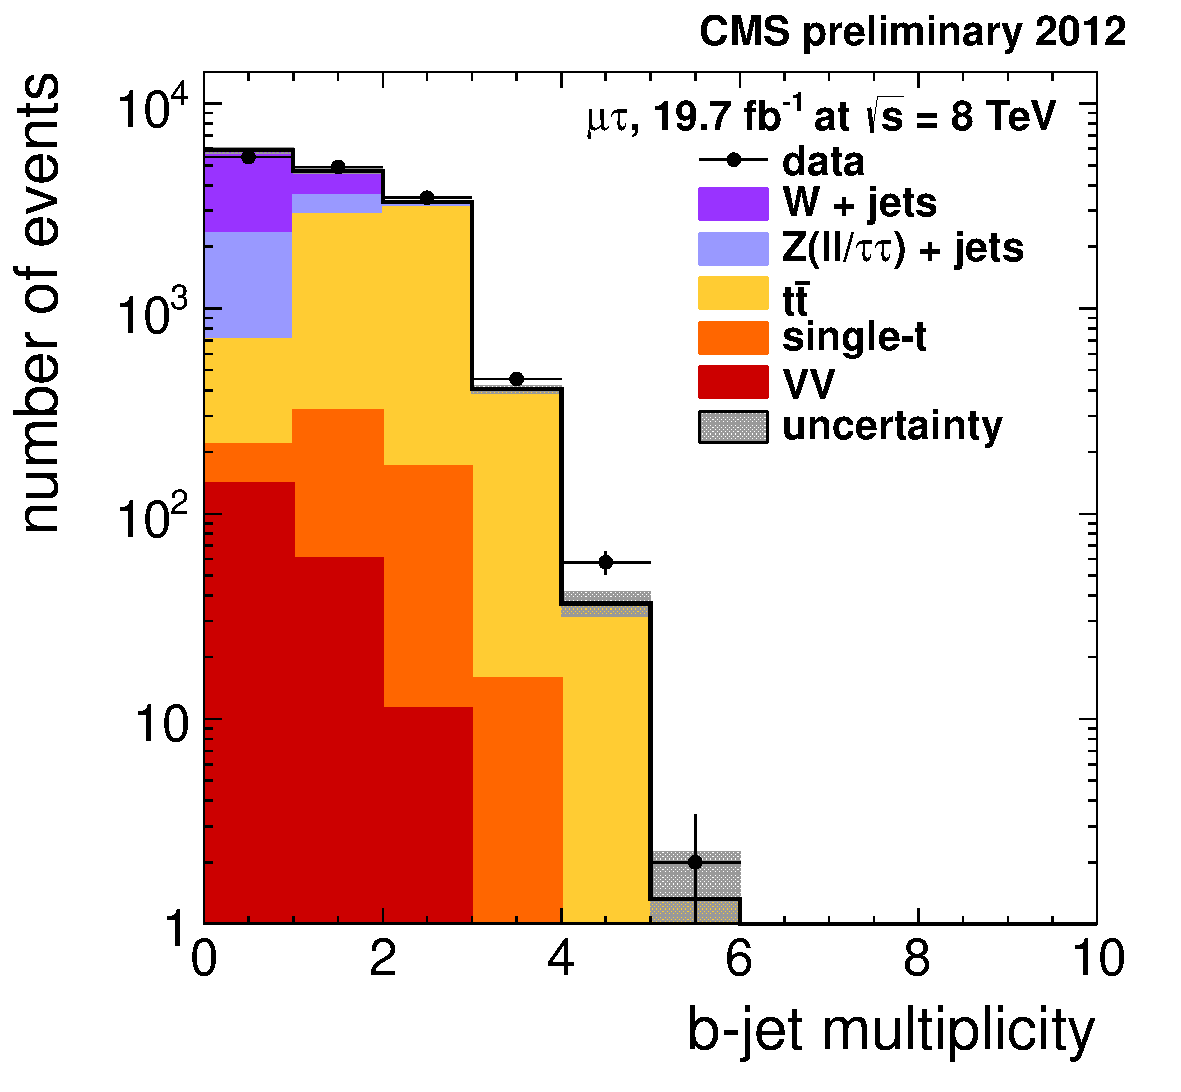
\includegraphics[width=0.465\textwidth]{figures/mutau/preselection/nbjet.pdf} \\
    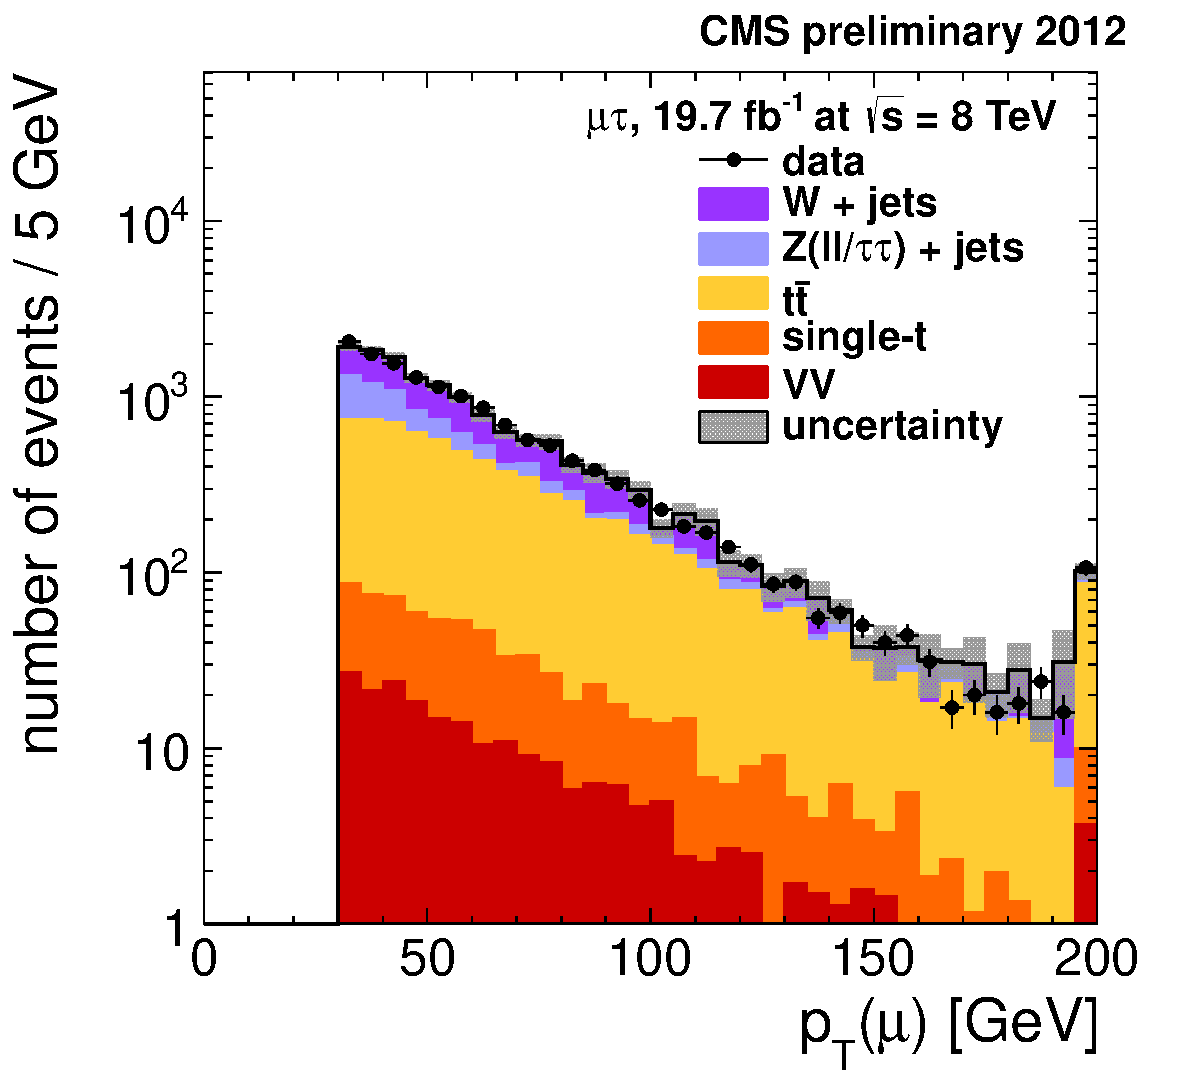
\includegraphics[width=0.465\textwidth]{figures/mutau/preselection/ptmu.pdf}
    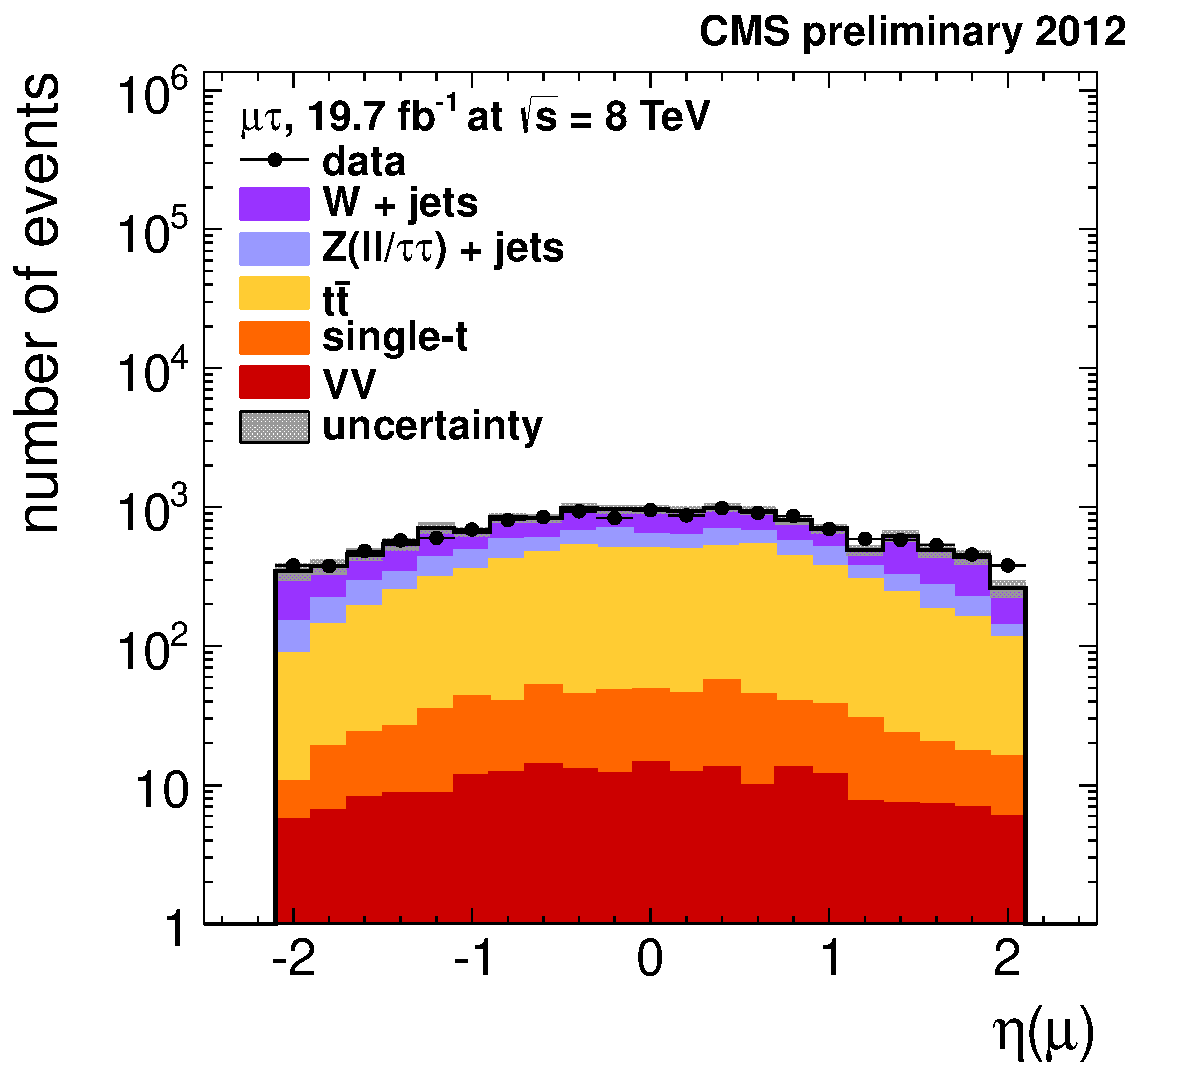
\includegraphics[width=0.465\textwidth]{figures/mutau/preselection/etamu.pdf} \\
    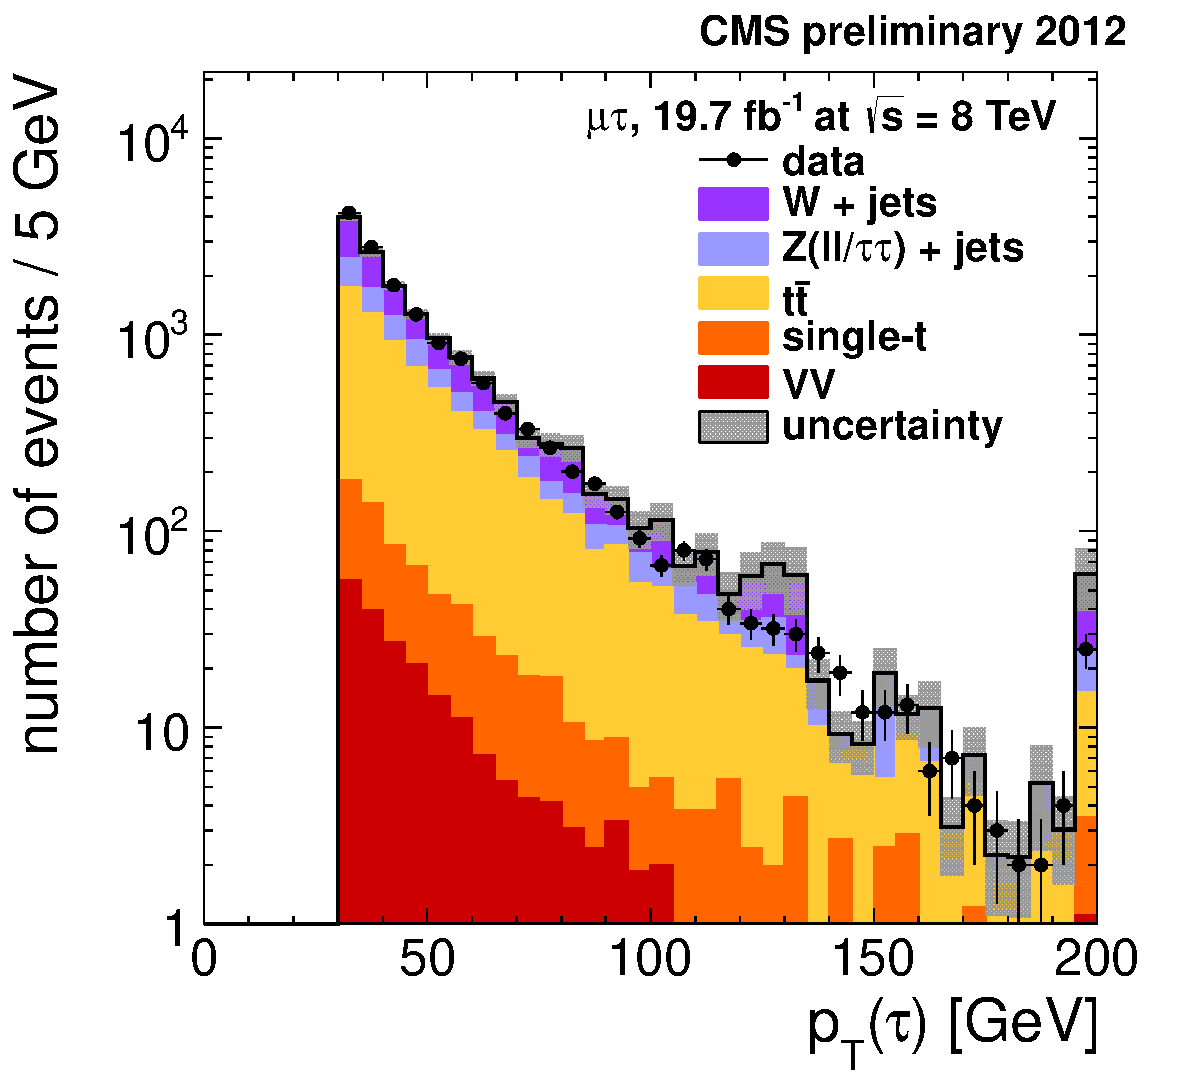
\includegraphics[width=0.465\textwidth]{figures/mutau/preselection/pttau.pdf}
    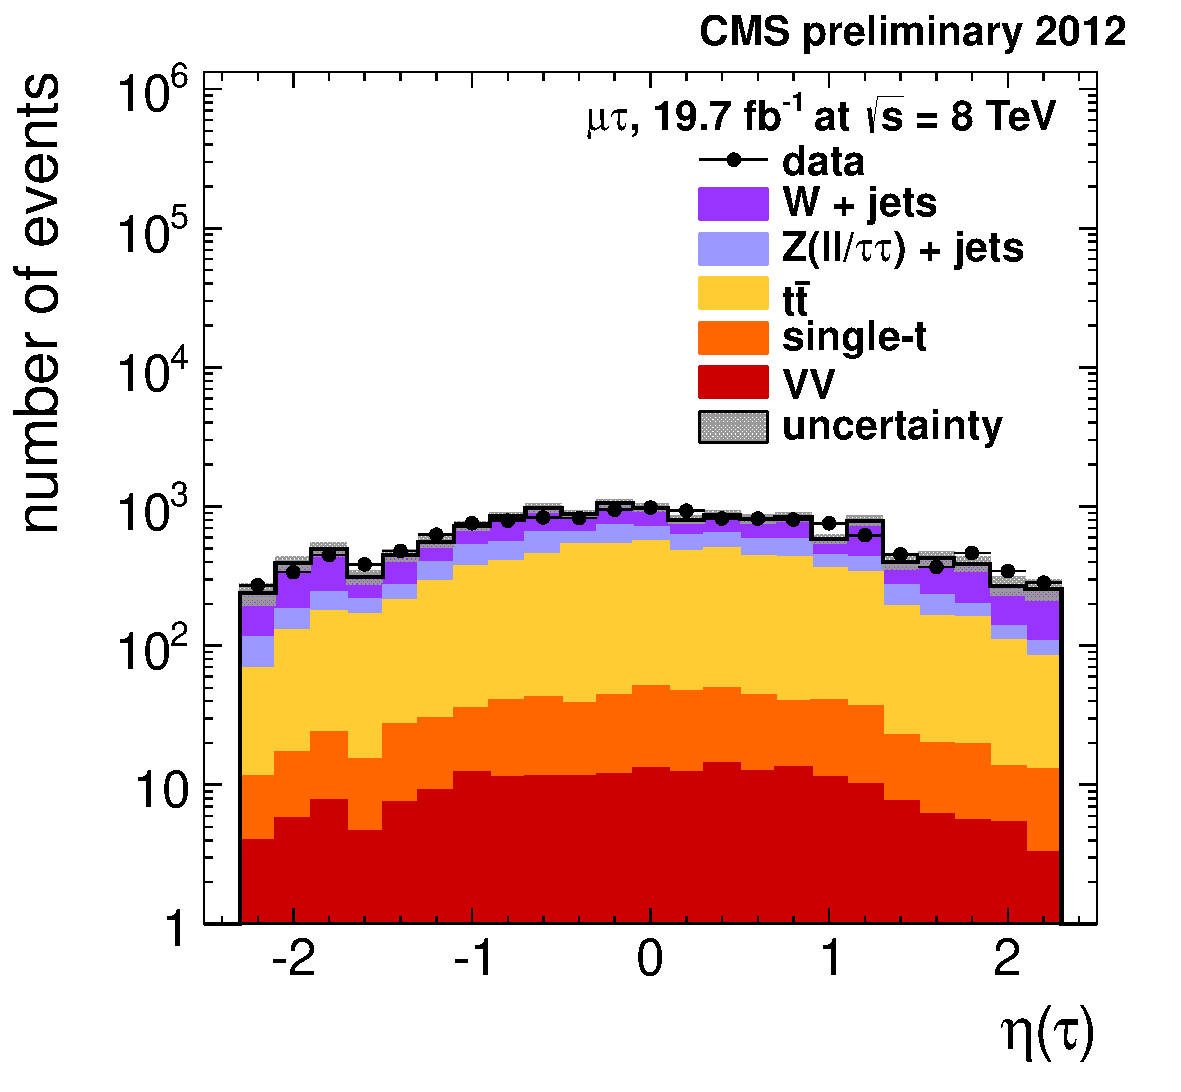
\includegraphics[width=0.465\textwidth]{figures/mutau/preselection/etatau.pdf}
    \caption{Plots of various kinematic quantities comparing observed data and simulated backgrounds in the \mutau channel after the preselection: the visible mass of the muon and hadronic tau (top left), the number of b-tagged jets (top right), the \pt (left) and $\eta$ (right) of the muon (middle) and hadronic tau (bottom). The uncertainty band reflects the statistical uncertainty in the simulated backgrounds.}
    \label{fig:preselmutau}
  \end{center}
\end{figure}

\begin{table}[hbt]
  \begin{center}
    \begin{tabular}{|l|c||c|}
      \hline
      & \etau channel & \mutau channel \\
      \hline
      \W+jets                         &  $4221.6 \pm 188.1$   & $4846.3 \pm 233.6 $ \\
      \Zttll+jets                     &  $4766.7 \pm 85.1$    & $2369.1 \pm 80.7  $ \\
      \ttbar                          &  $6272.2 \pm 65.5$    & $6430.5 \pm 69.8  $ \\
      Single t                        &  $462.9 \pm 14.4$     & $512.3 \pm 16.0   $ \\
      VV                              &  $223.4 \pm 4.4$      & $212.5 \pm 4.6    $ \\
      QCD multijets                   &  $(2452.6 \pm 512.1)$ & ---                 \\ 
      \hline                                                  
      Total Bkg. (no QCD)             & $15946.8 \pm 232.9$   & $14370.8 \pm 257.3$ \\
      \hline                                                  
      \hline                                                  
      Data                            & $18177$               & $14351$             \\
      \hline
    \end{tabular}
    \caption{The simulated background and observed event yields after the preselection in the \etau and \mutau channels. The statistical uncertainties are given for each simulated background. The contribution from the QCD multijets process is not taken into account in the total background yield. }
    \label{tab:eventyieldpresel}
  \end{center}
\end{table}

%\clearpage

\subsection{Main Selection}

A preselected event satisfies the main selection if at least one of the selected jets in the event is b-tagged. Though the expected final state from the signal includes two b-jets, it was found that requiring b-tagging for only one jet improved the signal yield in comparison to the SM backgrounds. This is expected due to the reduced efficiency of applying the CSV algorithm for b-tagging multiple times per event. The second jet in the event may or may not be b-tagged. Plots comparing observed data to the simulated backgrounds after the main selection are shown in Figs. \ref{fig:mainseletau} and \ref{fig:mainselmutau}, and event yields are given in Table \ref{tab:eventyieldmainsel}.

At this stage of the selection, several new observables are introduced. The first is the visible mass of the hadronic tau and a jet, \MassTJ. There are two possible pairings of the light lepton and the hadronic tau with the two selected jets. The pairing is chosen to minimize the difference between \MassTJ and \MassLJ. In signal events, these two values are expected to be similar, as both sets of correctly-paired particles will originate from the same mother particles, leptoquarks or top squarks. However, the visible mass variables will not directly measure the true mass of the mother particles; some of the energy will be lost in the form of neutrinos produced in tau lepton decays. According to the simulation of the signal process, this minimization selects the correct pairing in approximately 70\% of events. This observable will be used in the final selection for the leptoquark search.

The second new variable is \ST, which is defined as the scalar sum of \pt for all final-state objects:
\begin{equation}
\label{eq:STLQ}
\ST(\text{LQ}) = \pt(\ell) + \pt(\tauh) + \pt(\text{b-jet}) + \pt(\text{jet}).
\end{equation}
As indicated in Eq. \eqref{eq:STLQ}, this definition of \ST is appropriate for the leptoquark search, which requires four objects in the final state: a light lepton, a hadronic tau, a b-tagged jet, and another jet. Figures \ref{fig:mainseletau} and \ref{fig:mainselmutau} show this version of \ST. An alternate definition appropriate for the top squark search, which has a slightly different final state, is given in Eq. \eqref{eq:STstop}.

\begin{figure}[hbtp]
  \begin{center}
    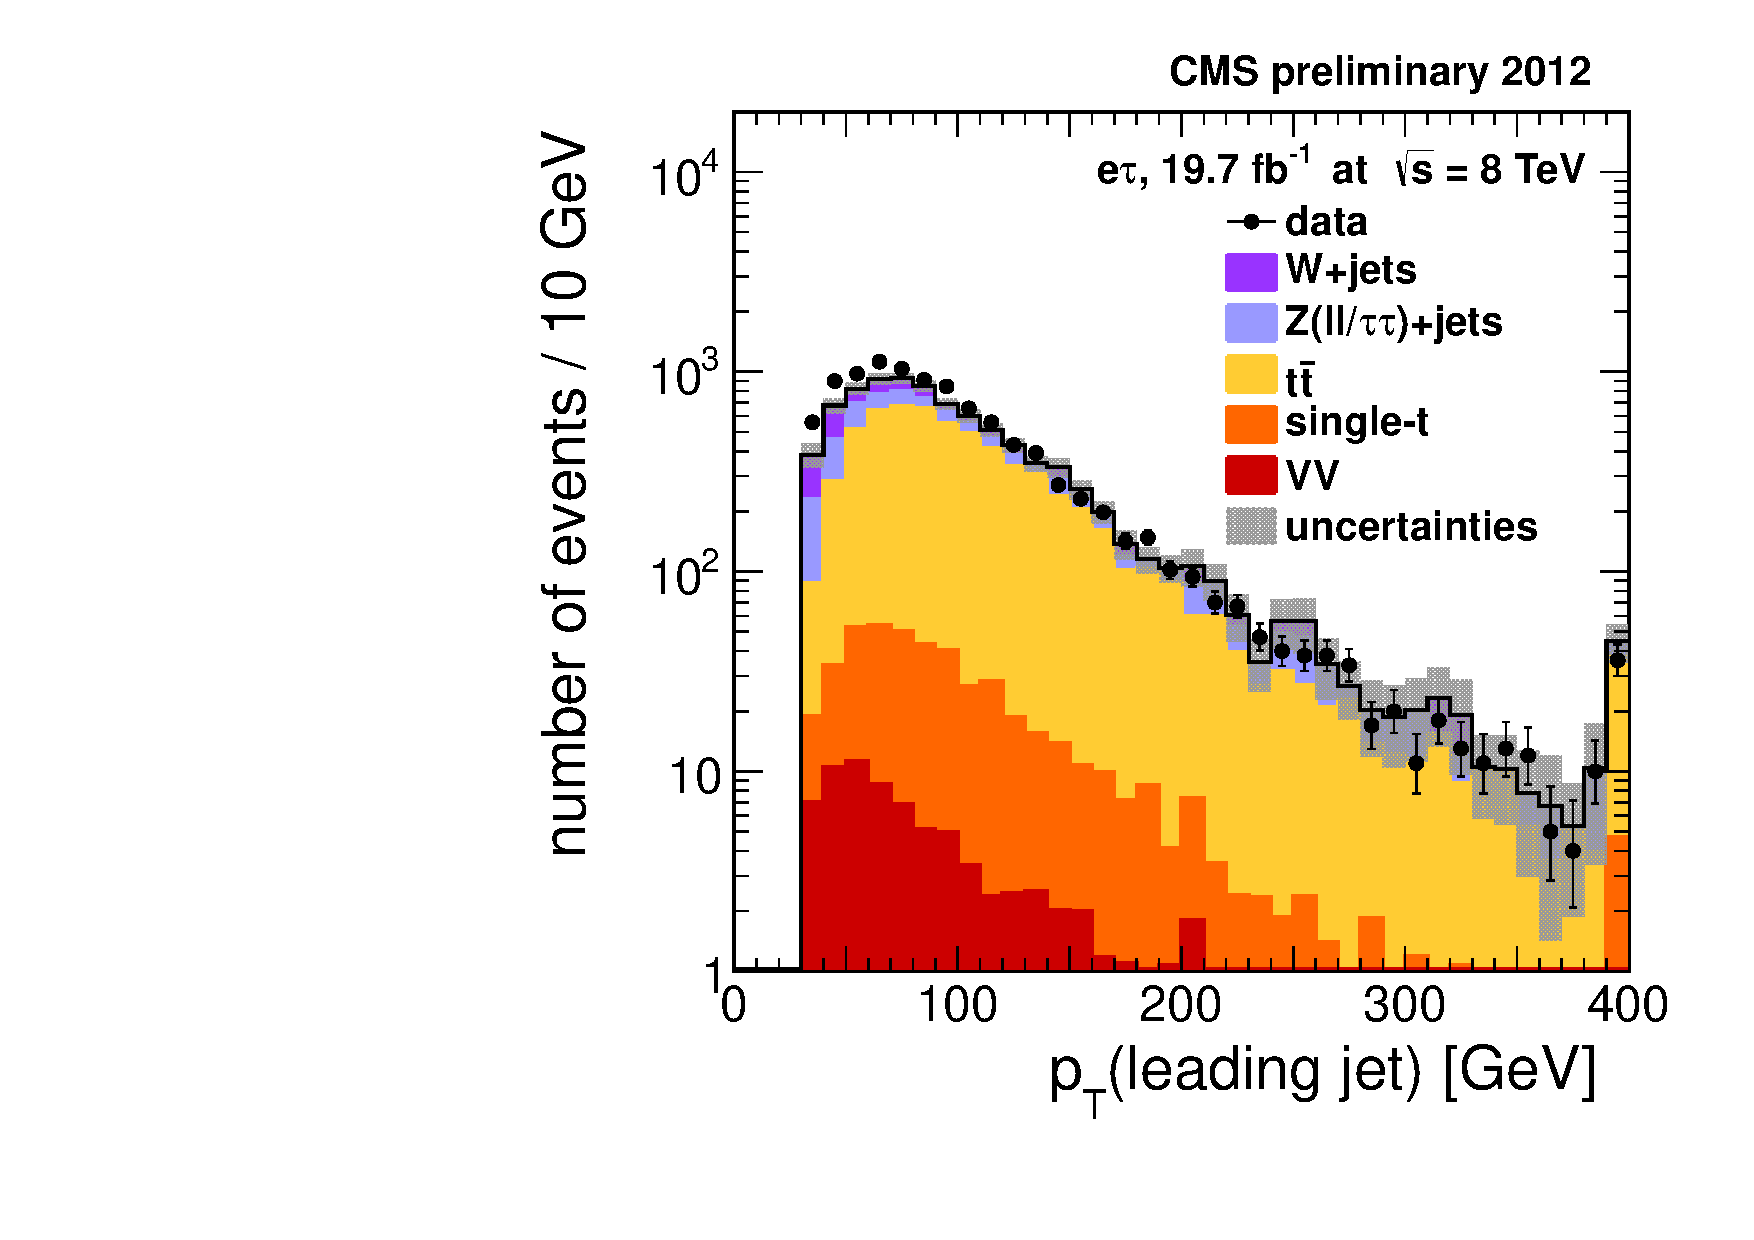
\includegraphics[width=0.49\textwidth]{figures/etau/jet1PtBTag.pdf}
    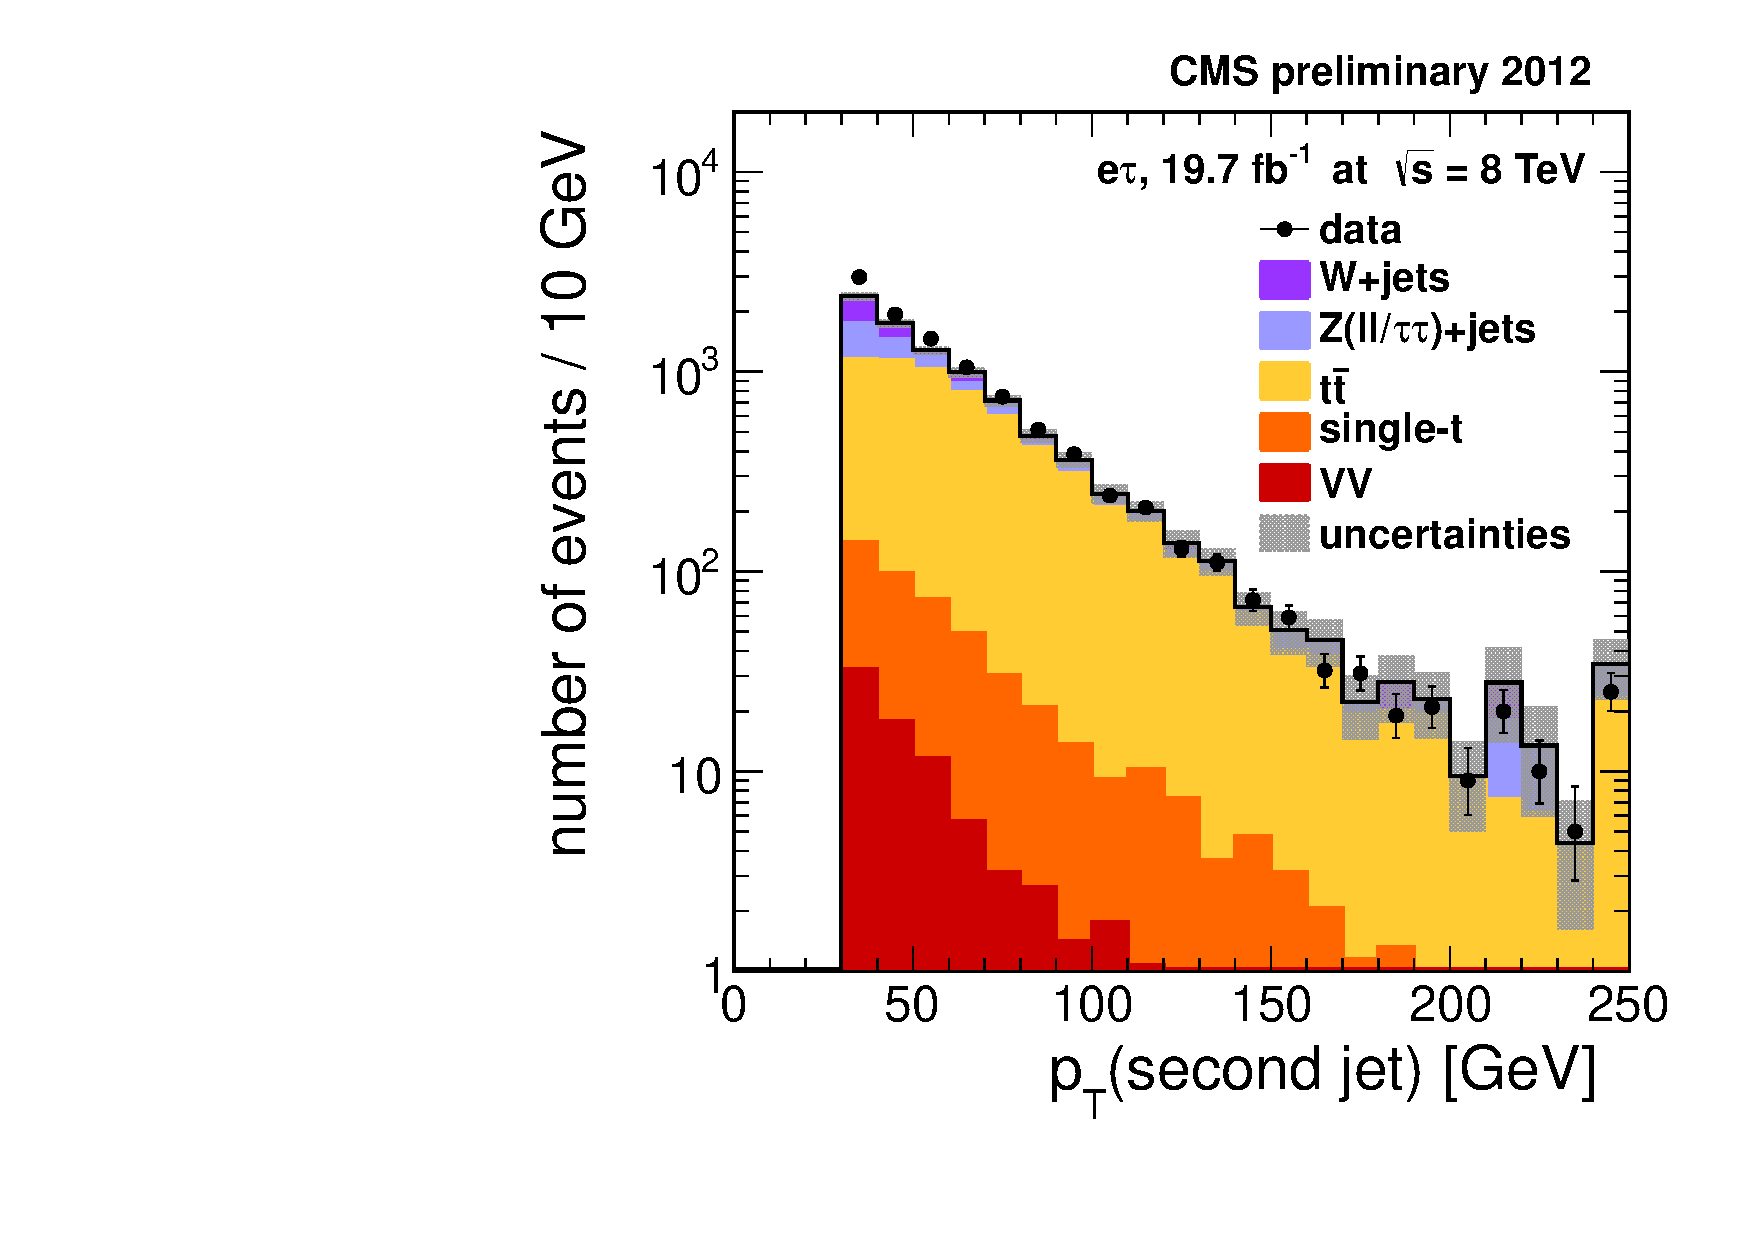
\includegraphics[width=0.49\textwidth]{figures/etau/jet2PtBTag.pdf} \\
    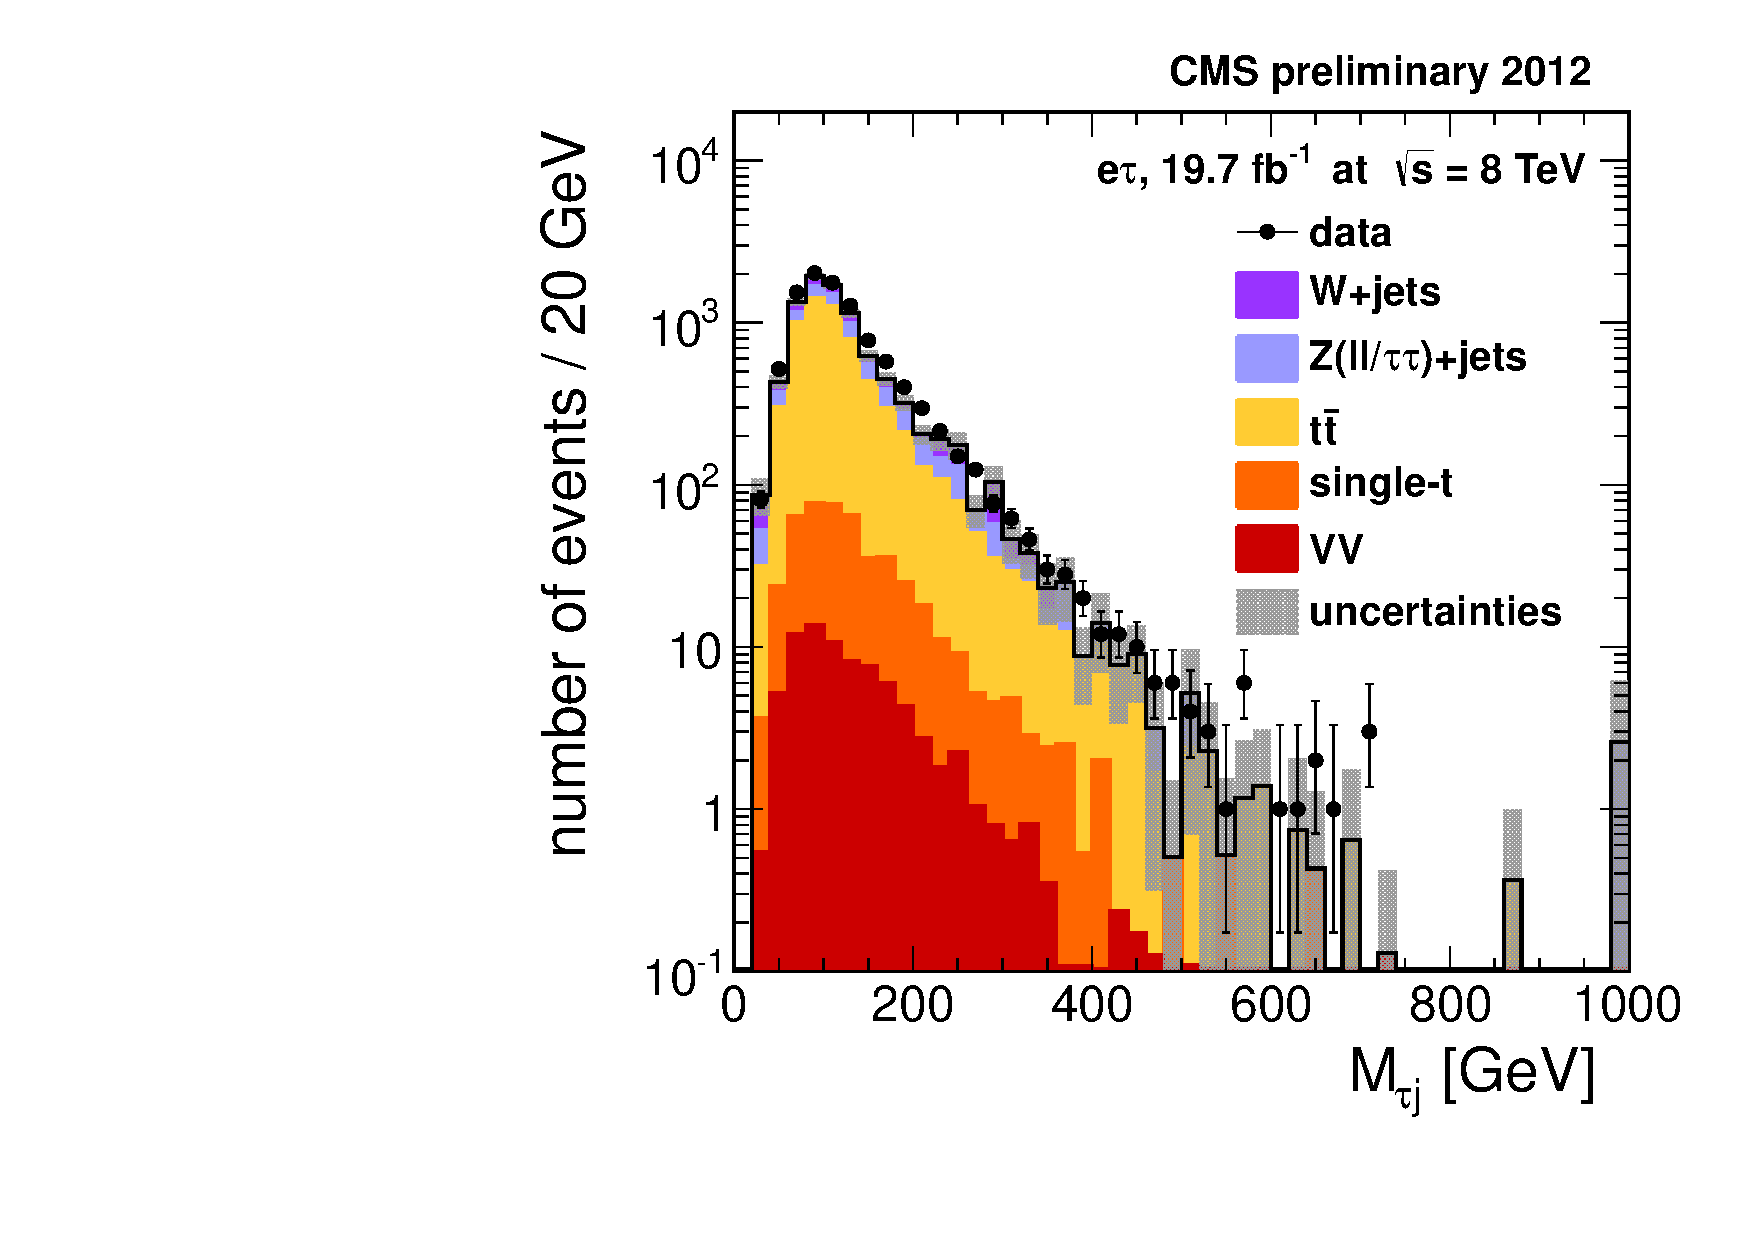
\includegraphics[width=0.49\textwidth]{figures/etau/finalMass.pdf}
    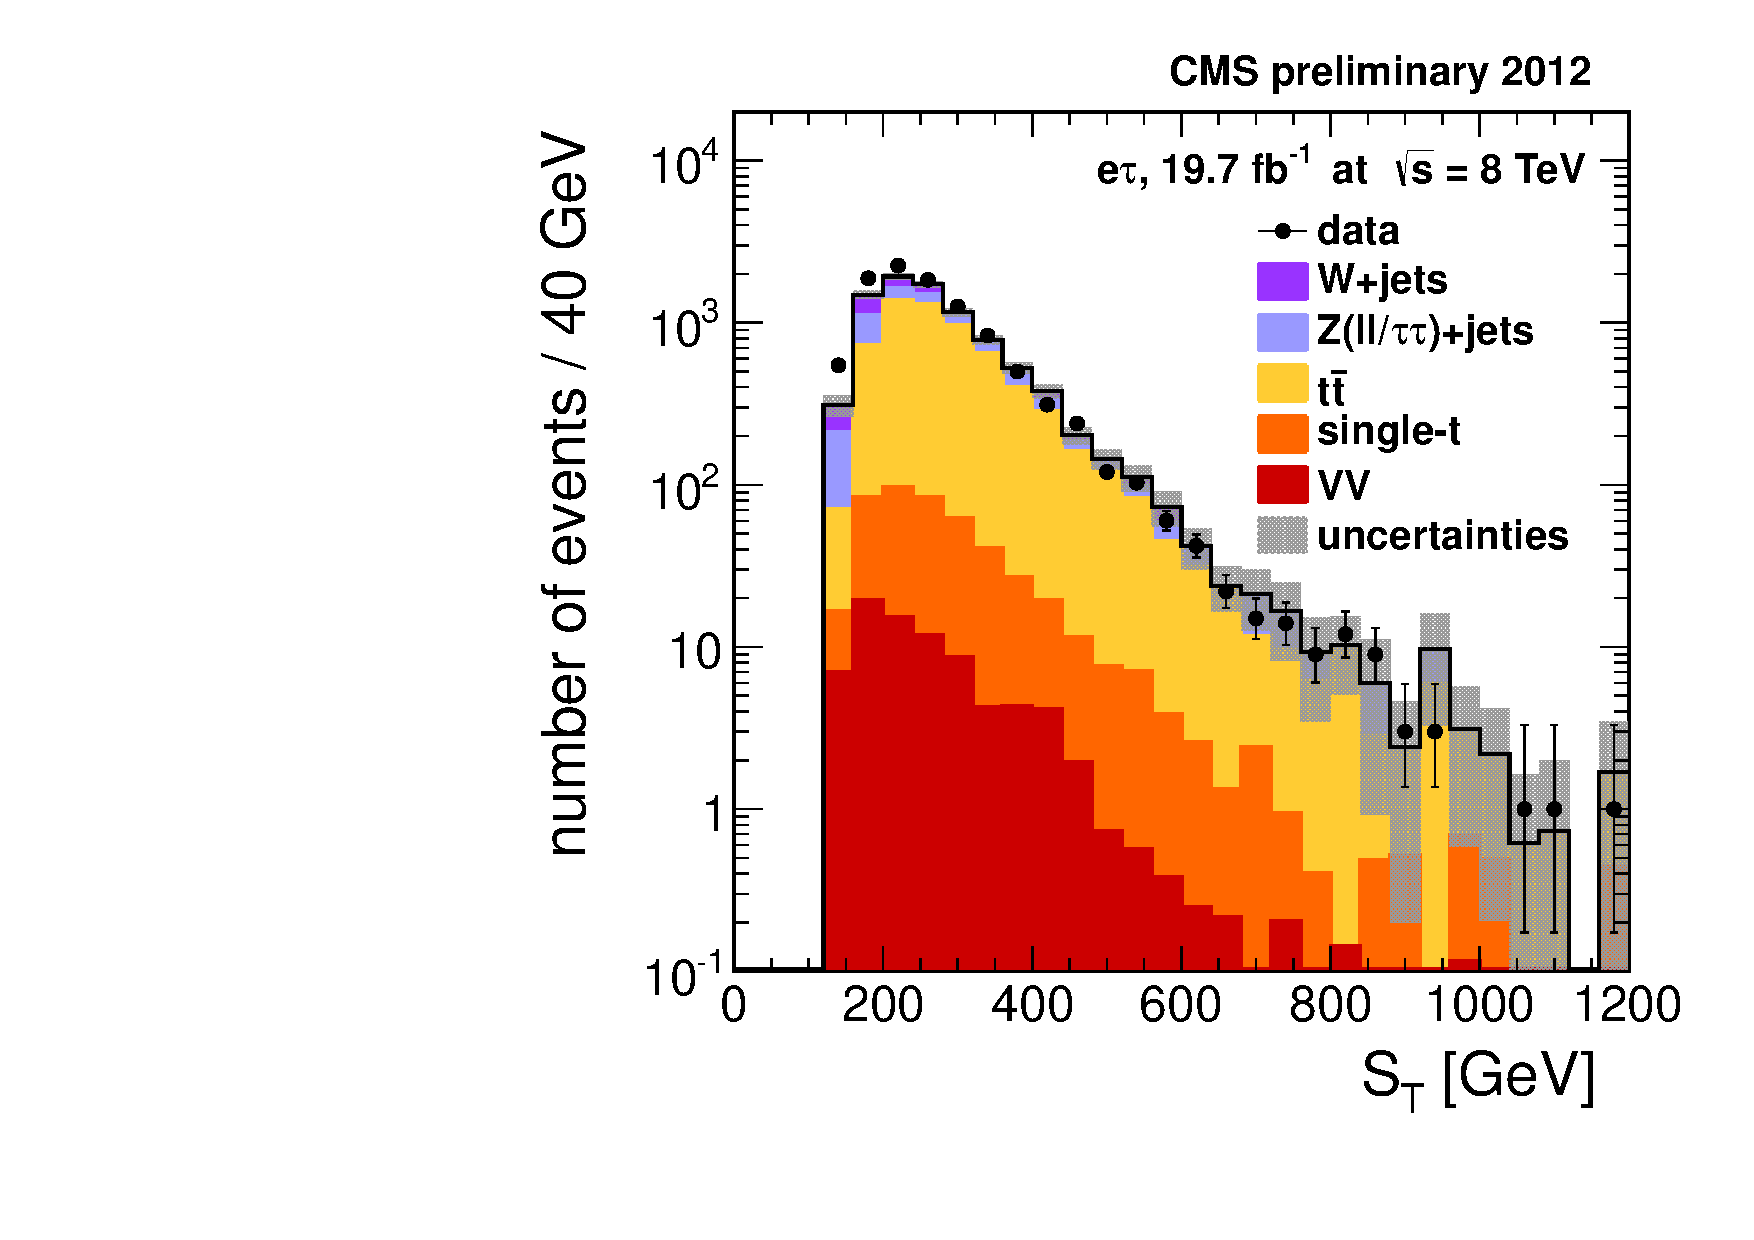
\includegraphics[width=0.49\textwidth]{figures/etau/STbjetBTag.pdf}
    \caption{Plots of various kinematic quantities comparing observed data and simulated backgrounds in the \etau channel after the main selection: the \pt spectra (top) of the first (left) and second (right) selected jets, \MassTJ (bottom left), and \ST (bottom right). The uncertainty band reflects the statistical uncertainty in the simulated backgrounds.}
    \label{fig:mainseletau}
  \end{center}
\end{figure}

\begin{figure}[hbtp]
  \begin{center}
    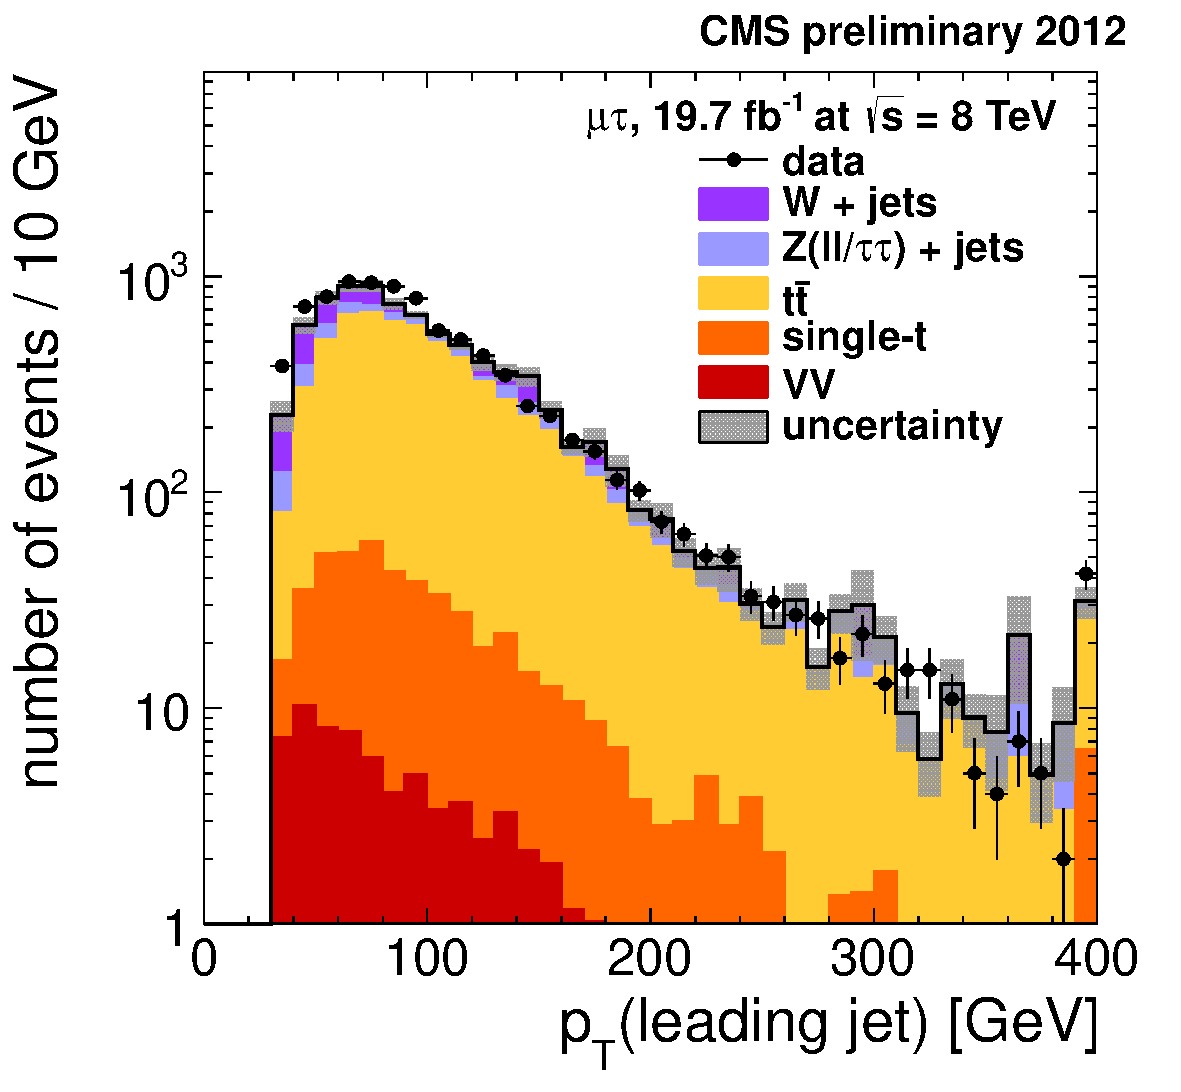
\includegraphics[width=0.49\textwidth]{figures/mutau/mainselection/leadseljetpt.pdf}
    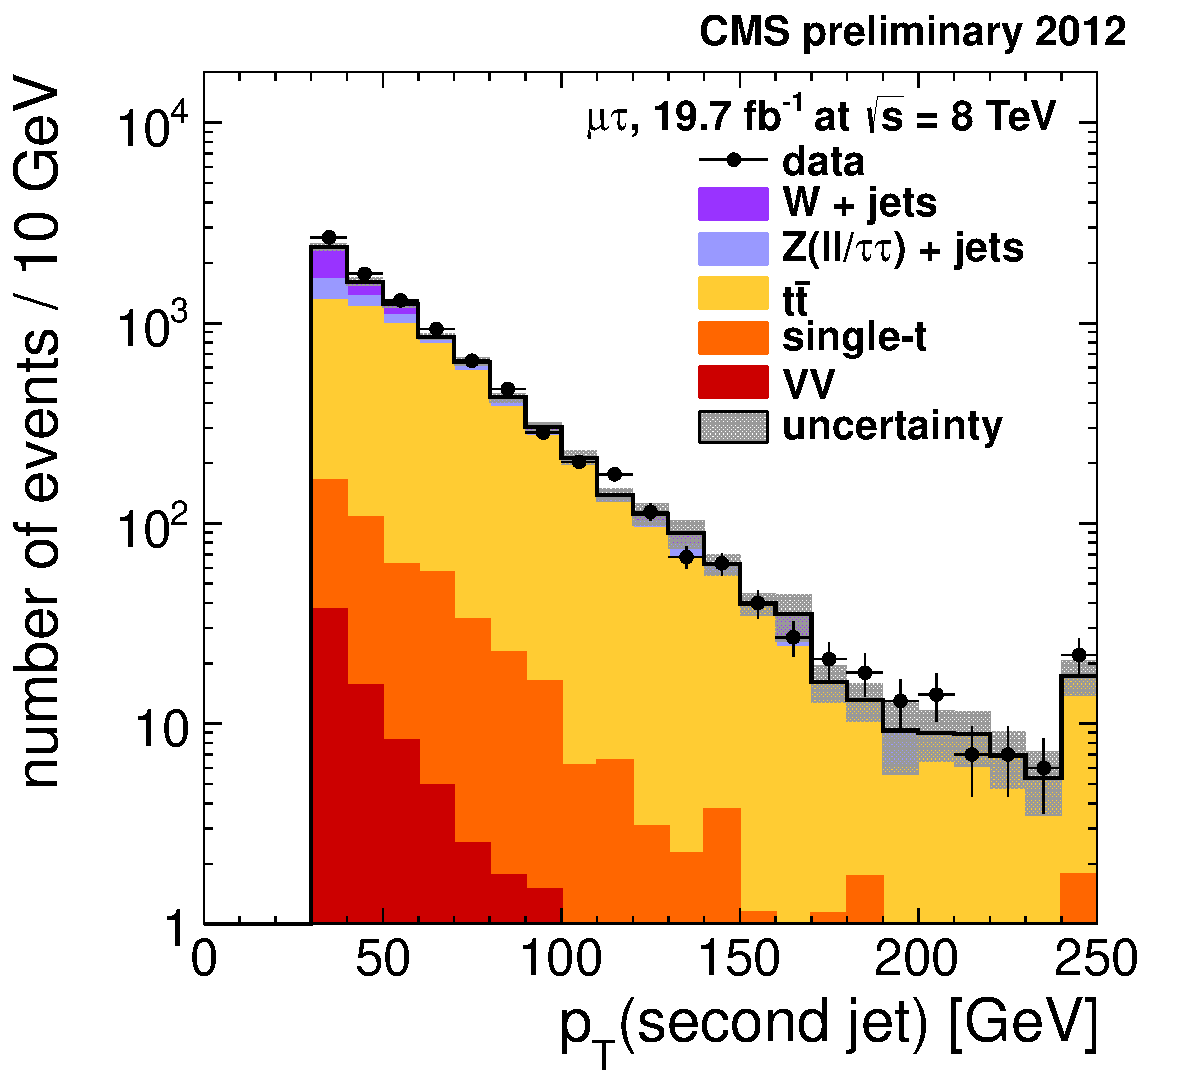
\includegraphics[width=0.49\textwidth]{figures/mutau/mainselection/secondseljetpt.pdf} \\
    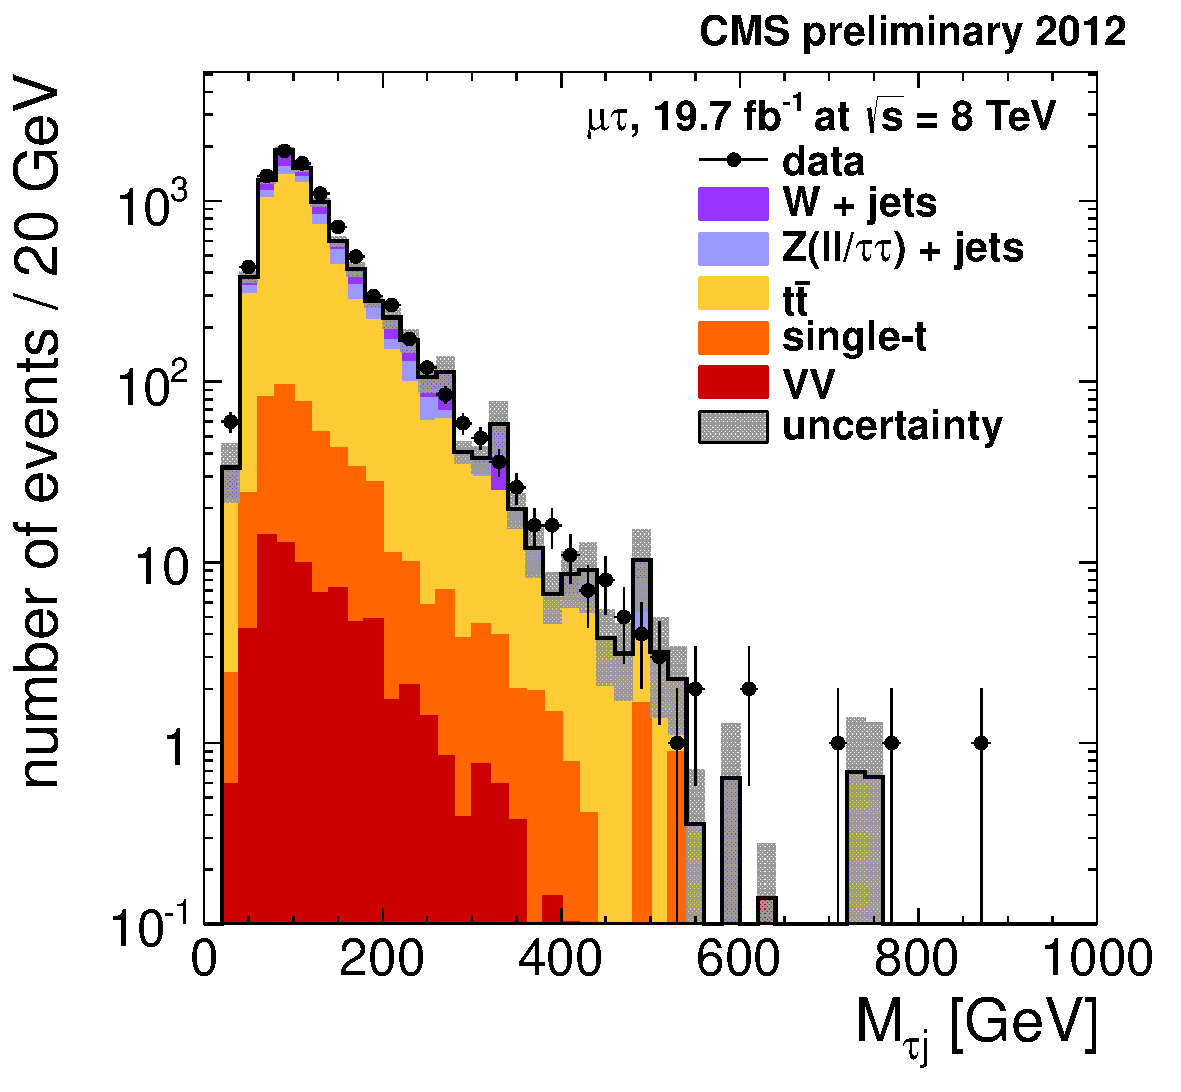
\includegraphics[width=0.49\textwidth]{figures/mutau/mainselection/masstaub.pdf}    
    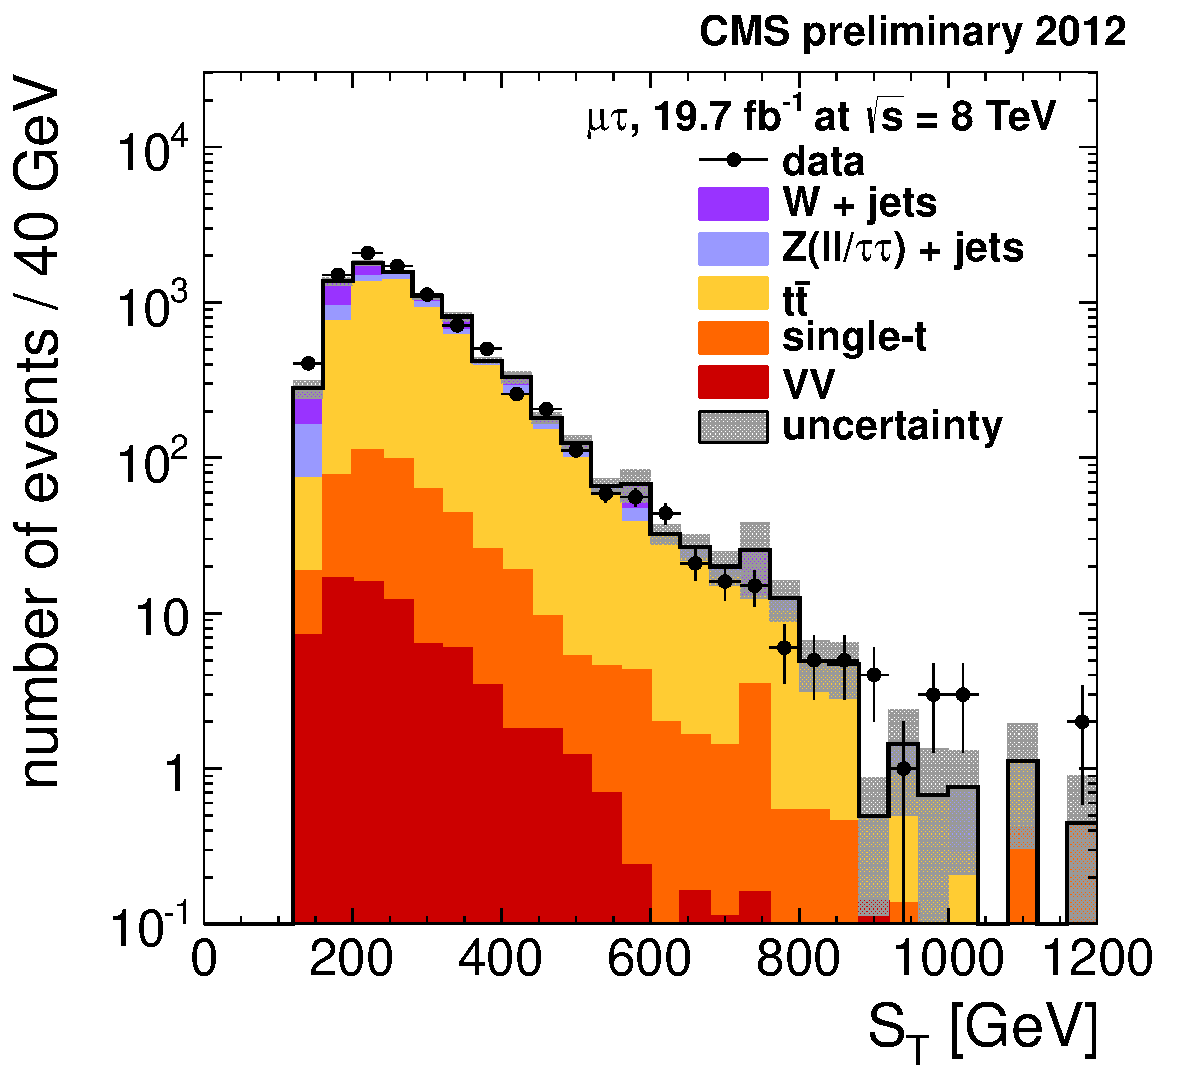
\includegraphics[width=0.49\textwidth]{figures/mutau/mainselection/st.pdf}
    \caption{Plots of various kinematic quantities comparing observed data and simulated backgrounds in the \mutau channel after the main selection: the \pt spectra (top) of the first (left) and second (right) selected jets, \MassTJ (bottom left), and \ST (bottom right). The uncertainty band reflects the statistical uncertainty in the simulated backgrounds.}
    \label{fig:mainselmutau}
  \end{center}
\end{figure}

\begin{table}[hbt]
  \begin{center}
    \begin{tabular}{|l|c||c|}
      \hline
      & \etau channel & \mutau channel \\
      \hline
      W + jets                        & $1201.9 \pm 104.0$   & $1285.8 \pm 122.7$ \\
      \Zttll + jets                   & $1534.0 \pm 49.5$    & $774.4 \pm 46.8  $ \\
      \ttbar                          & $5783.6 \pm 63.5$    & $5699.5 \pm 64.4 $ \\
      single-t                        & $390.2 \pm 13.46$    & $418.6 \pm 14.2  $ \\
      VV                              & $82.9 \pm 2.7$       & $74.1 \pm 2.7    $ \\
      QCD multijets                   & $(1226 \pm 131.0)$   & ---                \\
      \hline                                                 
      Total Bkg. (no QCD)             & $8992.6 \pm 141.2$   & $8252.3 \pm 147.0$ \\
      \hline                                                 
      \hline                                                 
      Data                            & 10113                & $8866$             \\
      \hline
    \end{tabular}
    \caption{The simulated background and observed event yields after the main selection in the \etau and \mutau channels. The statistical uncertainties are given for each simulated background. The contribution from the QCD multijets process is not taken into account in the total background yield. }
    \label{tab:eventyieldmainsel}
  \end{center}
\end{table}

%\clearpage

\subsection{Final Selections}

In the final stage of the selection for the leptoquark search, two additional requirements are applied. The selected hadronic tau must have $\pt>50\GeV$, and the selected events must have $\MassTJ>250\GeV$. This cut on the \MassTJ value is optimal for the expected limit based on the simulation for the entire range of leptoquark masses under consideration. The change in the kinematic properties of the signal for different mass values is taken into account when the \ST distribution is used to set $\text{CL}_{s}$ limits. The procedure for setting limits with a distribution is described in App. \ref{ch:limits}.

Slightly different final selection criteria are applied for the top squark search. Again, the selected hadronic tau must have $\pt>50\GeV$. Instead of a cut on \MassTJ, which is not a meaningful variable for the top squark $\lambda^{\prime}_{3jk}$ decay chain, the selected events are required to have $N_{\text{jets}}\geq5$. The expected final state of the top squark signal has $N_{\text{jet}}=6$, and though it was found that requiring $N_{\text{jets}}\geq6$ would maximize the expected limit based on the simulation, the number of both signal and background events passing that cut was greatly reduced. Because this would also reduce the number of events in the control regions used to estimate the major backgrounds, the corresponding increase in systematic uncertainty would render the limit indistinguishable from the $N_{\text{jets}}\geq5$ case. Thus, the slightly looser $N_{\text{jets}}$ cut was chosen. Given this cut, the \ST variable for the top squark search is defined as:
\begin{equation}
\label{eq:STstop}
\ST(\sTop) = \pt(\ell) + \pt(\tauh) + \pt(\text{b-jet}) + \sum_{i=1}^{4}\pt(\text{jet }i).
\end{equation}

Figure \ref{fig:finalcutscombined} shows the final selection variables for each search with both channels combined. Simulated signal distributions are added on top of the background to demonstrate the effect of the final selection cuts in removing background while preserving signal events. The common requirement $\pt(\tauh)>50\GeV$ is applied in these plots, and the major background yields are estimated from observed data. The background estimation techniques will be described in Sec. \ref{??}.

\begin{figure}[hbt]
  \begin{center}
    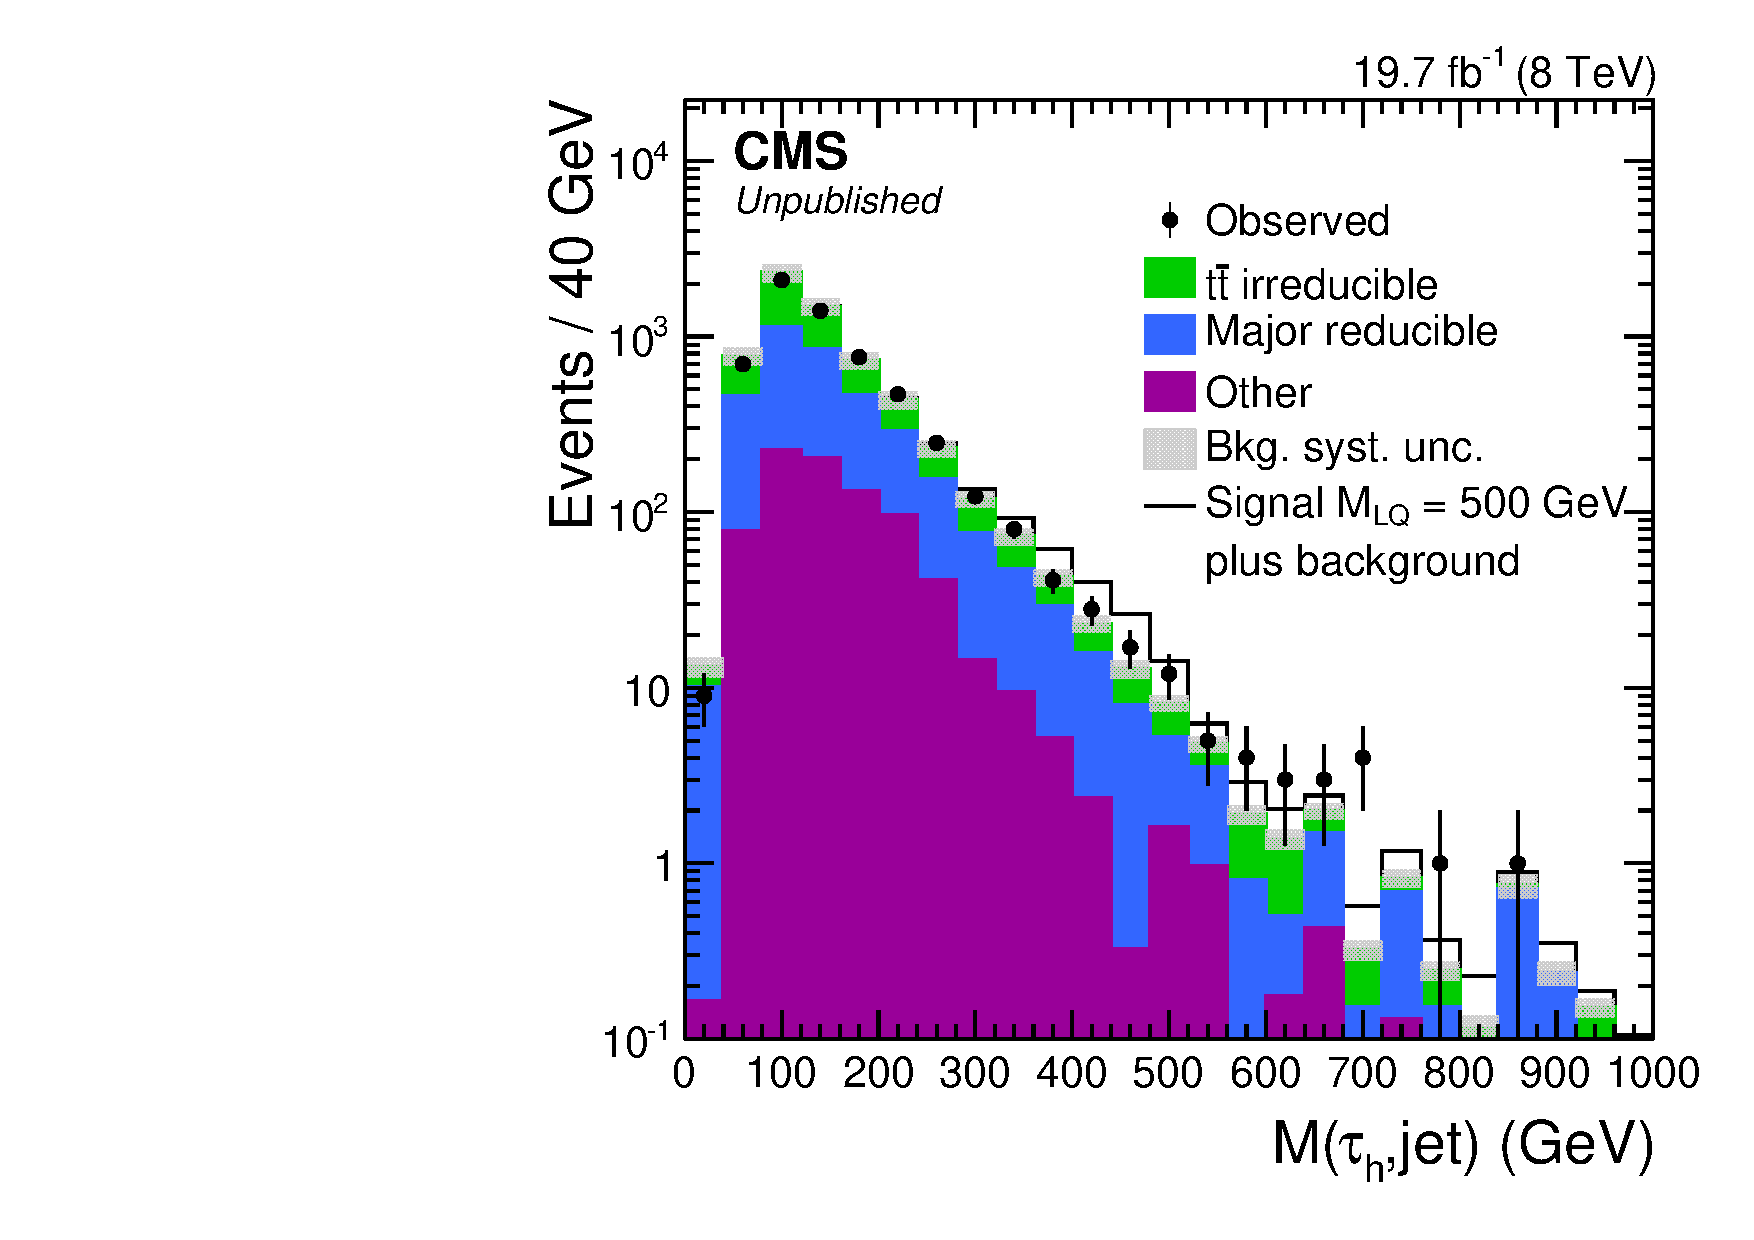
\includegraphics[width=0.49\textwidth]{figures/final/mtj_lq_log.pdf}
    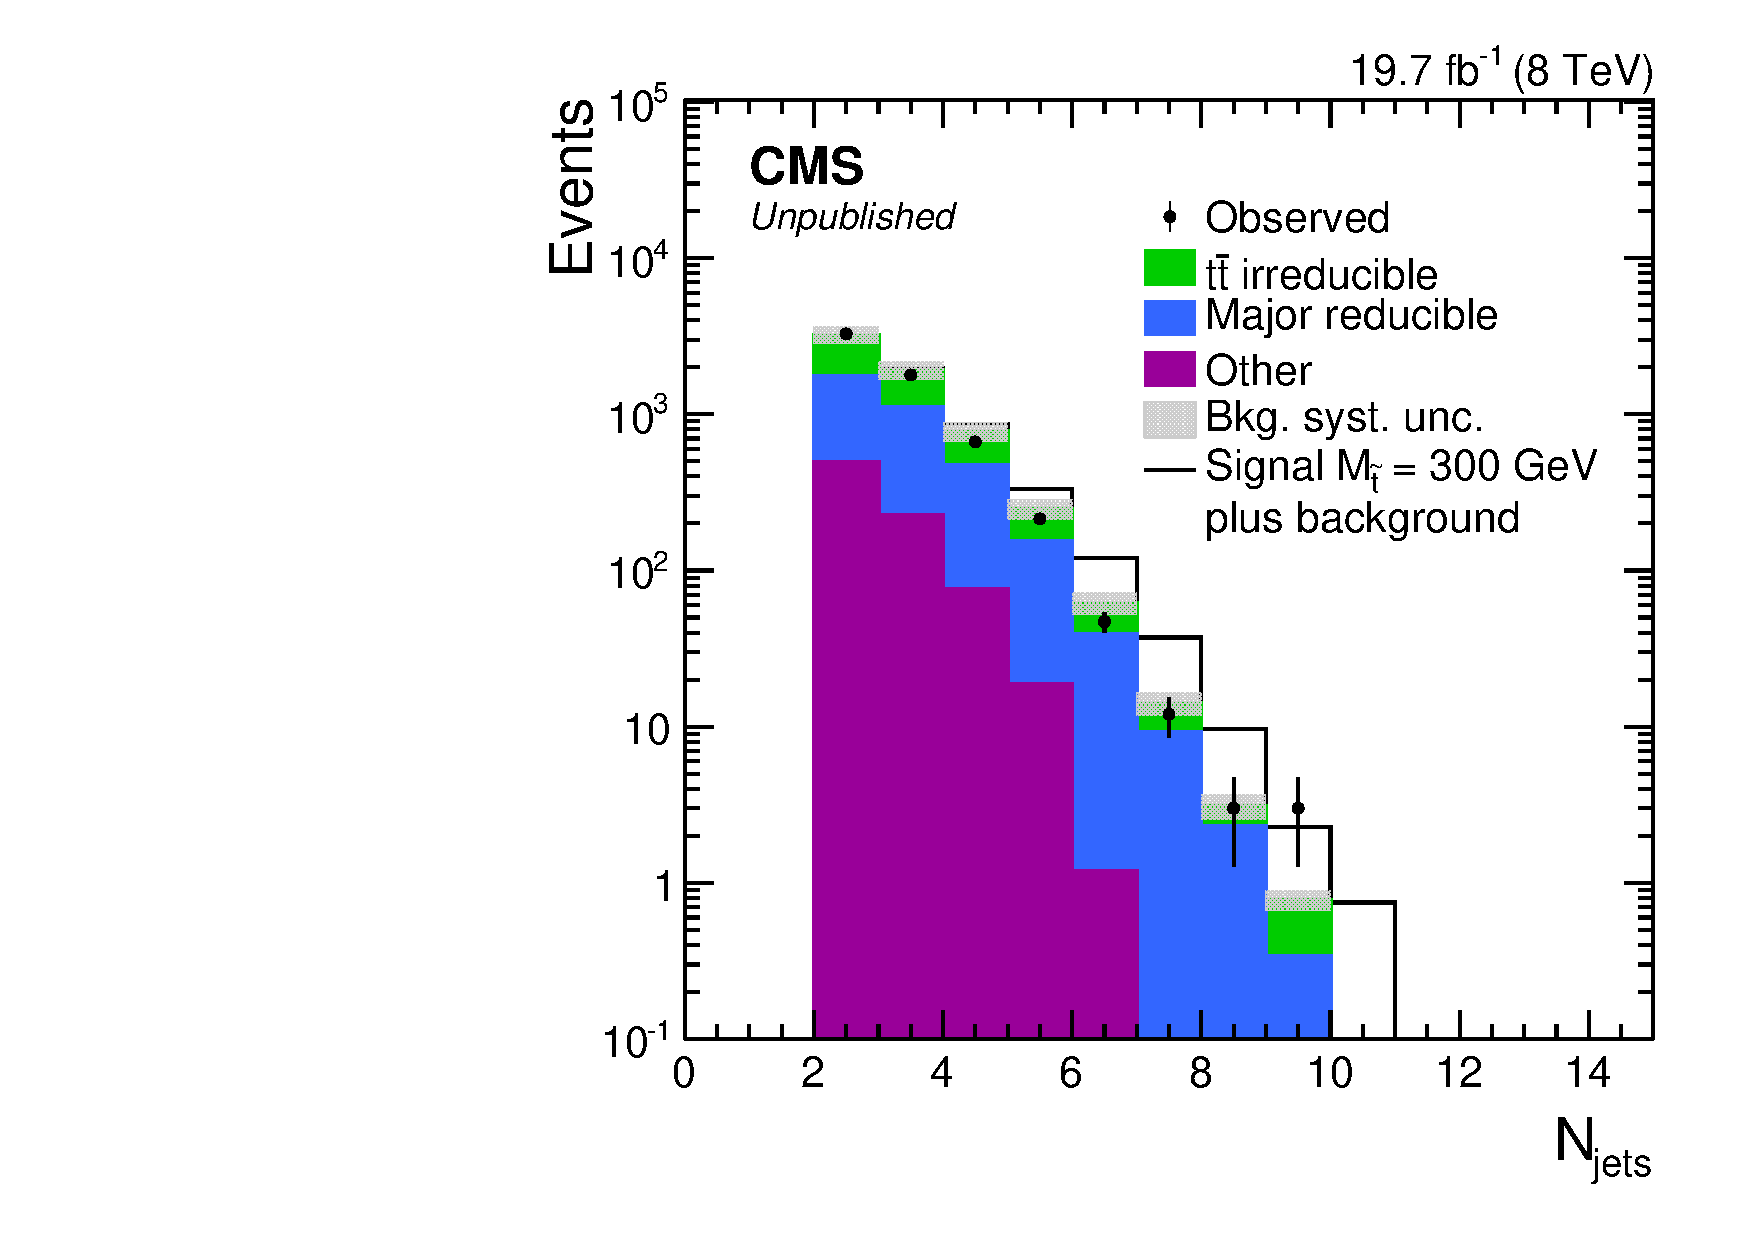
\includegraphics[width=0.49\textwidth]{figures/final/njets_lqd321_log.pdf}
    \caption{\MassTJ (left) and $N_{\text{jets}}$ (right) before the respective final selection cuts on these variables, with the \etau and \mutau channels combined. A signal sample for leptoquarks with a mass of 500\GeV (left) or top squarks with a mass of 300\GeV (right) is added on top of the background prediction. Both plots include the cut $\pt(\tauh)>50\GeV$ and the major backgrounds are estimated from observed data.}
    \label{fig:finalcutscombined}
  \end{center}
\end{figure}

\section{Background Estimations}

\subsection{Irreducible Background (ttbar)}

\subsection{Reducible Background (fake tau)}

\subsection{Reducible Background (QCD)}

\subsection{Other Backgrounds}

\section{Systematic Uncertainties}

\section{Results}
\chapter{Conclusions
\label{ch:conclusions}}

This dissertation has presented a search for pair production of third-generation scalar leptoquarks with each leptoquark decaying to a tau lepton and a bottom quark. The search used 19.7\fbinv of proton-proton collision data collected with the Compact Muon Solenoid experiment during the 2012 run of the Large Hadron Collider at a center-of-mass energy of $\sqrt{s}=8\TeV$. The existence of these leptoquarks is excluded at the 95\% confidence level for masses up to 740\GeV. This mass limit applies directly to pair production of top squarks decaying through the R-parity violating coupling $\lambda^{\prime}_{333}$, which has the same final-state signature and kinematic distributions as the third-generation scalar leptoquarks. This limit is a significant improvement over the previous limit of 530\GeV obtained using 7\TeV data \cite{CMSLQ3,ATLASLQ3}. Limits are also set for varying leptoquark branching fraction, with the area of low branching fraction constrained by a reinterpretation of a search for top squarks decaying to a top quark and a neutralino \cite{SUS-13-011}. 

The search is extended to cover top squarks undergoing a chargino-mediated decay involving the R-parity violating coupling $\lambda^{\prime}_{3jk}$, in which each top squark decays to a final state including a tau lepton, a bottom quark, and two light quarks. Top squarks undergoing this decay are excluded at the 95\% confidence level in the mass range 200--580\GeV. This is the first direct search for the top squark decay involving the coupling $\lambda^{\prime}_{3jk}$.

In 2015, Run 2 of the LHC will begin at approximately the design center-of-mass energy $\sqrt{s}=14\TeV$. This increase in energy corresponds to an order-of-magnitude increase in the pair production cross section for leptoquarks at high masses. The cross section for $\MLQ=1000\GeV$ will increase from $4.01\times10^{-4}\unit{pb}$ at $\sqrt{s}=8\TeV$ to $8.36\times10^{-3}\unit{pb}$ \cite{LQxsec}. With this significant increase in the cross section, the exclusion of leptoquarks at the \TeVns scale will be in reach with only a moderate amount of data \cite{LQPairHad}. Additionally, searches for single production of leptoquarks will become feasible, as the limits on the leptoquark Yukawa coupling only extend to the \TeVns scale \cite{Leurer:1993em, MuchAdo, LQreview}.

The searches for R-parity violating supersymmetry were motivated by the existing limits on R-parity conserving supersymmetry from searches requiring large missing transverse energy. The limits set in these searches, which are the most stringent to date for the selected couplings, similarly approach the high edge of the conditions for naturalness \cite{NaturalSUSY}. However, supersymmetry is not fully excluded yet; significant regions of the parameter space remain unexamined. Run 2 of the LHC will have a high potential for either the discovery or more complete exclusion of supersymmetry \cite{CMS:2013xfa}.

\appendix
   \titleformat{\chapter}
      {\normalfont\large}{Appendix \thechapter:}{1em}{}
\chapter{Full CLs Shape-Based Limits
\label{ch:limits}}

To set limits using the modified frequentist $\text{CL}_{s}$ procedure \cite{Read:CLs}, two hypotheses are defined. The first is the null or background-only hypothesis $H_{0}$ or $b$, and the second is the alternate or signal plus background hypothesis $H_{1}$ or $s+b$.

$\mathcal{P}(\theta; N_{H_{i}})$ is defined as the Poisson probability to observe $\theta$ events in data given the hypothesis $H_{i}$ which predicts $N_{H_{i}}$ events. This probability can be defined generally for the whole sample, but also per bin for a histogram of some quantity, e.g. \ST, and/or per channel.

To obtain this probability, it is necessary to integrate over all of the nuisance parameters:
\begin{equation}
\mathcal{P}(\theta; N_{H_{i}}) = \int \mbox{Poisson}(\theta; N_{H_{i}},\eta)f(\eta)d\eta
\end{equation}
where $f$ is the probability density function for the nuisance parameter $\eta$.

With those definitions, the test statistic $\mathcal{Q}$ is written as a ratio of likelihoods for a basic counting experiment:
\begin{equation}
\mathcal{Q} = \frac{\mathcal{P}(\theta; N_{H_{1}})}{\mathcal{P}(\theta; N_{H_{0}})}
\end{equation}
Splitting into \ST bins and two channels (\etau, \mutau) gives:
\begin{equation}
\mathcal{Q} = \prod_{i=\etau,\,\mutau}\prod_{j=0}^{n_{\text{bin}}} \frac{\mathcal{P}_{i,j}(\theta; N_{H_{1}})}{\mathcal{P}_{i,j}(\theta; N_{H_{0}})}
\end{equation}
For simplicity of computation, another form of the test statistic can be defined using the log likelihood ratio:
\begin{equation}
q = -2 \ln \mathcal{Q}
\end{equation}

To evaluate the test statistic as a function of the number of observed events $\theta$, many simulated pseudo-experiments are performed. For each hypothesis, $\theta$ is varied according to the probability distribution of that hypothesis, and the value of $\mathcal{Q}$ (or $q$) is kept for each $\theta$ value. To get $\mathcal{Q}$ for the actual number of observed events, $\mathcal{Q}_{\text{obs}}$, the same procedure is followed using $\theta=N_{\text{obs}}$. The $\text{CL}_{s+b}$ and $\text{CL}_{b}$ variables correspond to the probability for $\mathcal{Q_{\text{obs}}}$ to be greater than the $\mathcal{Q}$ values obtained for the hypotheses $H_1$ and $H_0$, respectively. When using $q$ as the test statistic, the observed value should be smaller than the value for the hypothesis. A visual example of these variables is shown in Fig. \ref{fig:q}.
\begin{align}
\text{CL}_{s+b} &= \mathcal{P}(\mathcal{Q}_{H_{1}} \leq \mathcal{Q}_{\text{obs}}) = \mathcal{P}(q_{H_{1}} \geq q_{\text{obs}}) \\
\text{CL}_{b} &= \mathcal{P}(\mathcal{Q}_{H_{0}} \leq \mathcal{Q}_{\text{obs}}) = \mathcal{P}(q_{H_{0}} \geq q_{\text{obs}}) \\
\text{CL}_{s} &= \text{CL}_{s+b}/\text{CL}_{b}
\end{align}

\begin{figure}[hbt]
\begin{center}
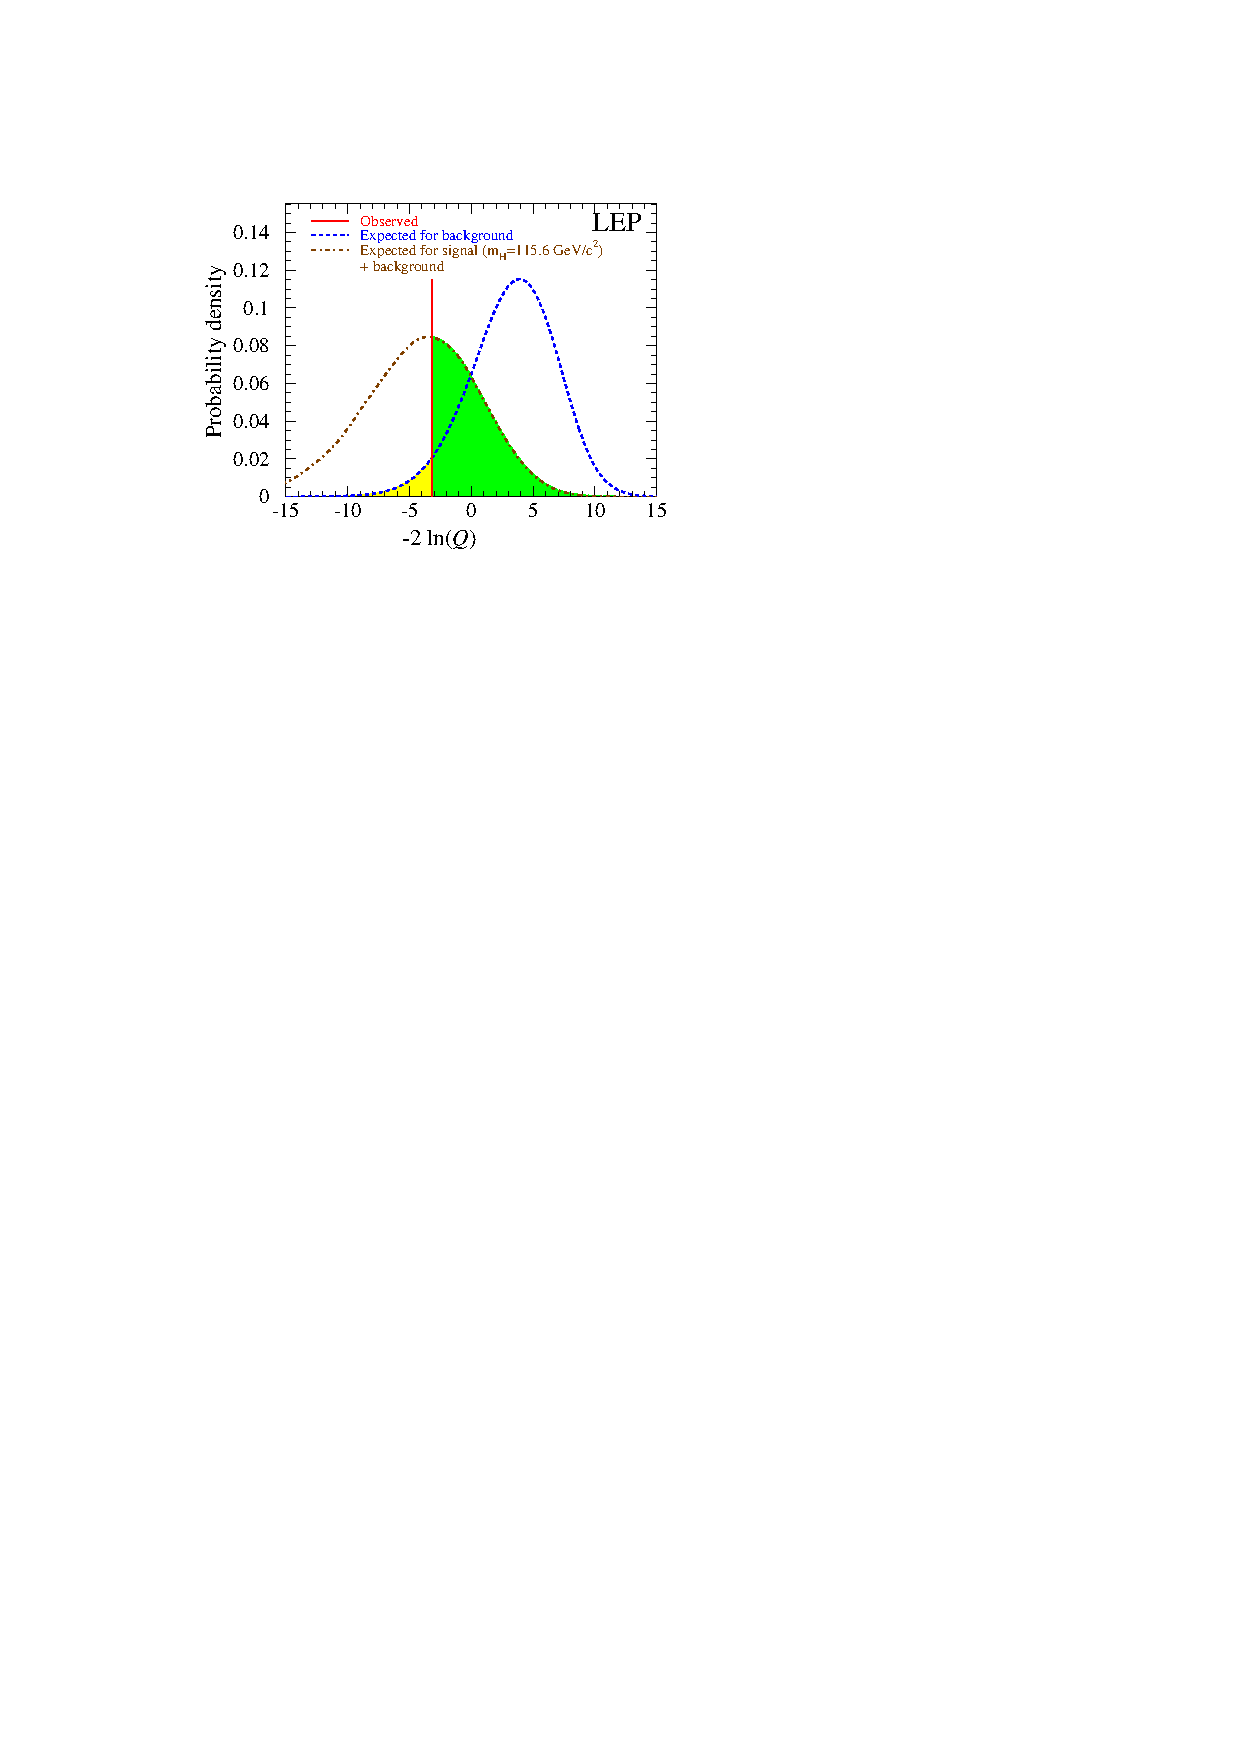
\includegraphics[width=0.95\textwidth]{figures/g21013-fig1.pdf}
\caption{Comparison of the observed value (red line) to the probability densities for $H_{0}$ (background only, blue line) and $H_{1}$ (signal + background, brown line) as a function of the log likelihood ratio. Green area: $\text{CL}_{s+b}$, yellow area: $1-\text{CL}_{b}$. From \cite{Read:presentation}.}
\label{fig:q}
\end{center}
\end{figure}

To set a mass limit on the signal hypothesis, the calculation of $\text{CL}_{s}$ is repeated for different signal masses. Masses with $\text{CL}_{s} < 1 - \alpha$ are excluded at the $\alpha$ confidence level, typically 95\%.
\chapter{Event Displays
\label{ch:displays}}

\section{Leptoquark Search}

Figure \ref{fig:lq-evt1} shows the two-dimensional display in the transverse ($r$-$\phi$) plane and the three-dimensional display for the highest \ST observed event in the \mutau channel of the leptoquark search. Figure \ref{fig:lq-evt2} shows the same displays for the second-highest \ST observed event. The kinematic properties of the selected particles in those events are listed in Table \ref{tab:lq-evt}.

\begin{table}[htbp]
  \centering
    \begin{tabular}{|r|l|r|r|r|}
      \hline
      \multicolumn{1}{|c|}{\ST $[\GeVns]$} & \multicolumn{1}{c|}{Particle} & \multicolumn{1}{c|}{\pt $[\GeVns]$} & \multicolumn{1}{c|}{$\eta$} & \multicolumn{1}{c|}{$\phi$} \\
      \hline
      1444.6                               & $\mu$                         &   92.0                              & $-0.84$                     & $-0.16$ \\
                                           & \tauh                         &   87.8                              & $ 0.43$                     & $ 1.76$ \\
                                           & b-jet                         &  125.2                              & $ 1.63$                     & $ 1.57$ \\
                                           & jet                           & 1139.6                              & $-0.60$                     & $-2.72$ \\
      \hline
      1012.1                               & $\mu$                         &  293.6                              & $-0.49$                     & $-0.13$ \\
                                           & \tauh                         &   57.0                              & $ 0.37$                     & $-1.03$ \\
                                           & b-jet                         &   77.4                              & $ 1.92$                     & $-1.98$ \\
                                           & jet                           &  584.1                              & $-0.06$                     & $ 3.08$ \\
      \hline
    \end{tabular}
    \caption{The kinematic properties of the selected particles for the two highest \ST observed events in the \mutau channel of the leptoquark search.}    
    \label{tab:lq-evt}
\end{table}

\begin{figure}[hbtp]
\begin{center}
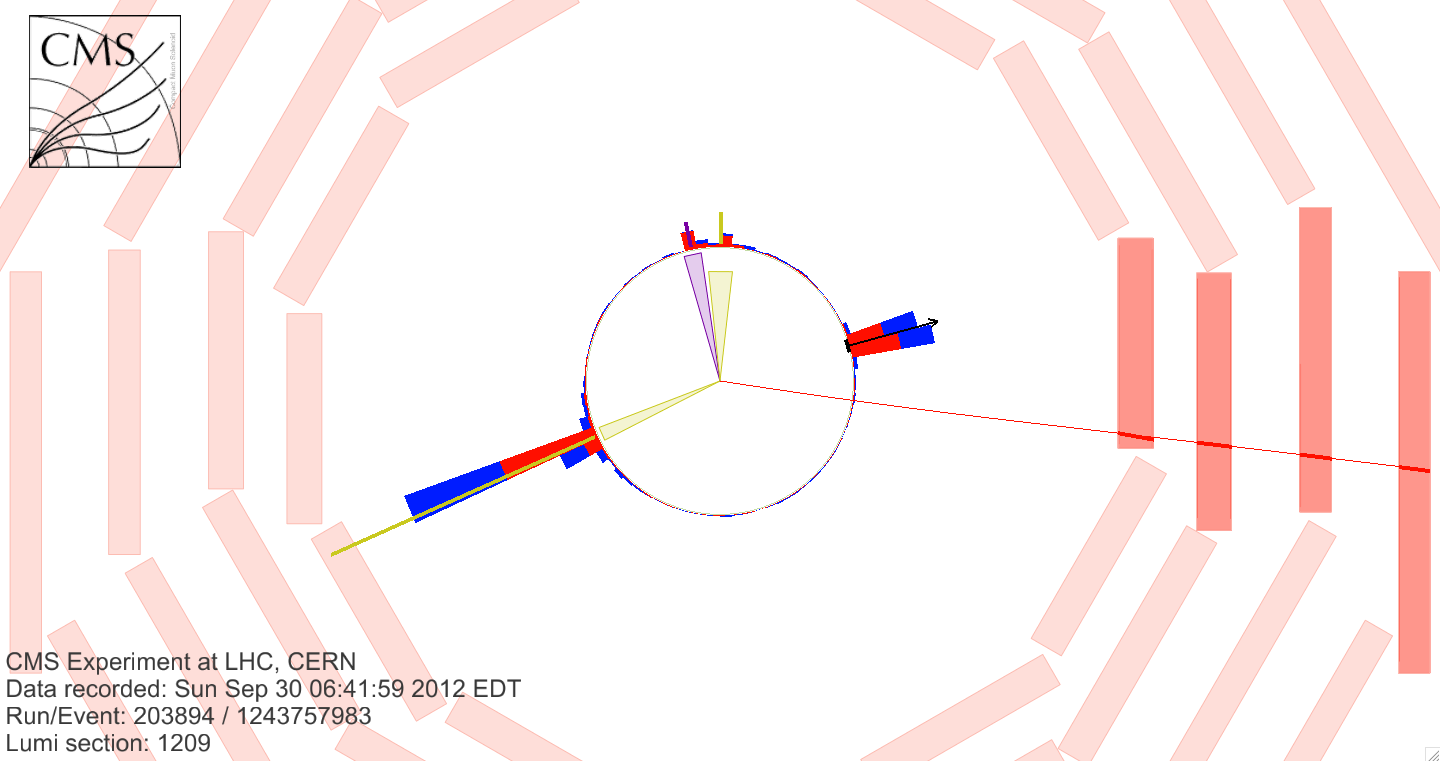
\includegraphics[width=0.95\textwidth]{figures/eventdisplays/LQ_evt1_rphi.png}
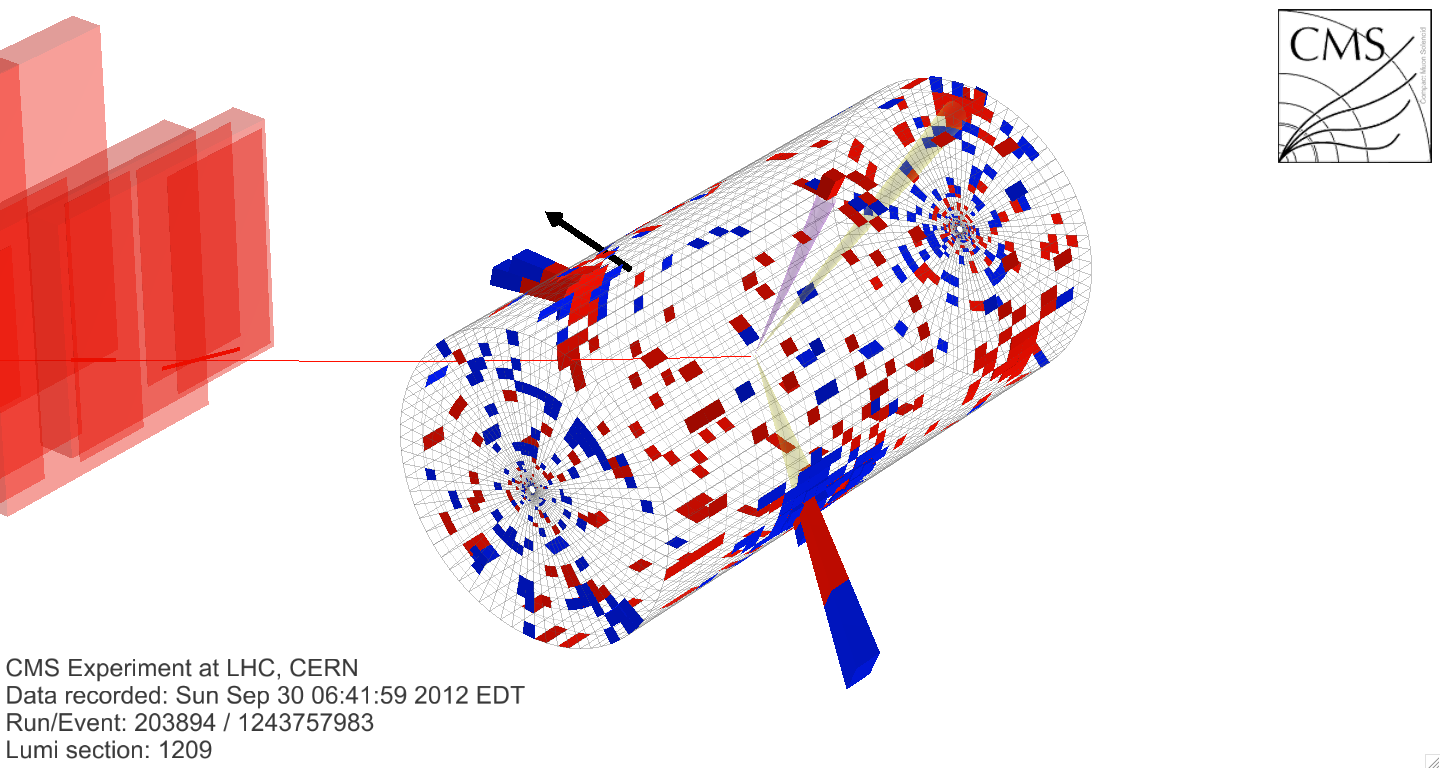
\includegraphics[width=0.95\textwidth]{figures/eventdisplays/LQ_evt1_3D.png}
\caption{A two-dimensional display in the transverse ($r$-$\phi$) plane (top) and a three-dimensional display (bottom) for the highest \ST observed event in the \mutau channel of the leptoquark search. The red line represents the muon, and the associated red rectangles represent the muon chamber hits. The purple cone represents the hadronic tau, and the yellow cones represent the jets. The black arrow indicates the \met in the event, while the ECAL and HCAL energy deposits are represented as red and blue towers, respectively. }
\label{fig:lq-evt1}
\end{center}
\end{figure}

\begin{figure}[hbtp]
\begin{center}
\includegraphics[width=0.95\textwidth]{figures/eventdisplays/LQ_evt2_rphi.png}
\includegraphics[width=0.95\textwidth]{figures/eventdisplays/LQ_evt2_3D.png}
\caption{A two-dimensional display in the transverse ($r$-$\phi$) plane (top) and a three-dimensional display (bottom) for the second-highest \ST observed event in the \mutau channel of the leptoquark search. The red line represents the muon, and the associated red rectangles represent the muon chamber hits. The purple cone represents the hadronic tau, and the yellow cones represent the jets. The black arrow indicates the \met in the event, while the ECAL and HCAL energy deposits are represented as red and blue towers, respectively. }
\label{fig:lq-evt2}
\end{center}
\end{figure}

\clearpage

\section{Top Squark Search}

Figure \ref{fig:lqd-evt1} shows the two-dimensional display in the transverse ($r$-$\phi$) plane and the three-dimensional display for the highest \ST observed event in the \mutau channel of the top squark search. Figure \ref{fig:lqd-evt2} shows the same displays for the second-highest \ST observed event. The kinematic properties of the selected particles in those events are listed in Table \ref{tab:lqd-evt}.

\begin{table}[htbp]
  \centering
    \begin{tabular}{|r|l|r|r|r|}
      \hline
      \multicolumn{1}{|c|}{\ST $[\GeVns]$} & \multicolumn{1}{c|}{Particle} & \multicolumn{1}{c|}{\pt $[\GeVns]$} & \multicolumn{1}{c|}{$\eta$} & \multicolumn{1}{c|}{$\phi$} \\
      \hline
      1586.2                               & $\mu$                         &   92.0                              & $-0.84$                     & $-0.16$ \\
                                           & \tauh                         &   87.8                              & $ 0.43$                     & $ 1.76$ \\
                                           & b-jet                         &  125.2                              & $ 1.63$                     & $ 1.57$ \\
                                           & jet 1                         & 1139.6                              & $-0.60$                     & $-2.72$ \\
                                           & jet 2                         &   63.5                              & $-0.05$                     & $-2.77$ \\
                                           & jet 3                         &   42.9                              & $ 1.10$                     & $-2.87$ \\
                                           & jet 4                         &   35.2                              & $-1.69$                     & $-2.19$ \\
      \hline
      1136.3                               & $\mu$                         &  313.1                              & $-0.09$                     & $-1.18$ \\
                                           & \tauh                         &   53.7                              & $ 1.83$                     & $ 0.89$ \\
                                           & b-jet                         &  156.0                              & $-0.09$                     & $ 1.52$ \\
                                           & jet 1                         &  325.3                              & $ 0.00$                     & $ 2.49$ \\
                                           & jet 2                         &  123.1                              & $-0.67$                     & $-1.57$ \\
                                           & jet 3                         &  103.0                              & $-0.59$                     & $ 1.93$ \\
                                           & jet 4                         &   62.2                              & $-0.62$                     & $-2.32$ \\
      \hline
    \end{tabular}
    \caption{The kinematic properties of the selected particles for the two highest \ST observed events in the \mutau channel of the top squark search.}    
    \label{tab:lqd-evt}
\end{table}

\begin{figure}[hbtp]
\begin{center}
\includegraphics[width=0.95\textwidth]{figures/eventdisplays/LQD_evt1_rphi.png}
\includegraphics[width=0.95\textwidth]{figures/eventdisplays/LQD_evt1_3D.png}
\caption{A two-dimensional display in the transverse ($r$-$\phi$) plane (top) and a three-dimensional display (bottom) for the highest \ST observed event in the \mutau channel of the top squark search. The red line represents the muon, and the associated red rectangles represent the muon chamber hits. The purple cone represents the hadronic tau, and the yellow cones represent the jets. The black arrow indicates the \met in the event, while the ECAL and HCAL energy deposits are represented as red and blue towers, respectively. }
\label{fig:lqd-evt1}
\end{center}
\end{figure}

\begin{figure}[hbtp]
\begin{center}
\includegraphics[width=0.95\textwidth]{figures/eventdisplays/LQD_evt2_rphi.png}
\includegraphics[width=0.95\textwidth]{figures/eventdisplays/LQD_evt2_3D.png}
\caption{A two-dimensional display in the transverse ($r$-$\phi$) plane (top) and a three-dimensional display (bottom) for the second-highest \ST observed event in the \mutau channel of the top squark search. The red line represents the muon, and the associated red rectangles represent the muon chamber hits. The purple cone represents the hadronic tau, and the yellow cones represent the jets. The black arrow indicates the \met in the event, while the ECAL and HCAL energy deposits are represented as red and blue towers, respectively. }
\label{fig:lqd-evt2}
\end{center}
\end{figure}
\chapter{Table of Monte Carlo Datasets
\label{ch:datasets}}
\chapter{CMS Collaboration
\label{ch:collaboration}}

\renewcommand{\baselinestretch}{1}
\small\normalsize
\newpage
\bibliographystyle{lucas_unsrt} 
\bibliography{mybib}

\end{document}
